\documentclass[a4paper, twoside, 11pt]{book}

% ============
% = PACKAGES =
% ============
\usepackage[utf8]{inputenc}
\def\labelitemi{--} % dash in itemize
\usepackage{booktabs} % in table, use of toprule, midrule and bottomrule
\usepackage{rotating} % allow to rotate a table
\usepackage[Lenny]{fncychap} % chapter customized typo
\usepackage[vscale=0.75,
            hscale=0.75, 
            hmarginratio=5:4, 
            vmarginratio=1:1, 
            marginparsep=5pt, 
            marginparwidth=2cm, 
            headheight=15pt]{geometry} % layout
\usepackage{graphicx} % graphics
\usepackage{amsmath, amssymb} % math
\usepackage{algorithm, algorithmic} %algorithms
\usepackage[tight]{subfigure} % subfigures
\usepackage{xspace} % space at end of macros
\usepackage{fancyhdr} % head of chapters (using lhead)
\usepackage{tabularx, caption}
\usepackage[square, sort&compress, numbers]{natbib}
\makeatletter
% \def\NAT@spacechar{\ }% OLD
\def\NAT@spacechar{~}% NEW
\makeatother
\usepackage{pdfpages} % to insert a pdf right into the thesis
\usepackage[pagebackref=true, final, colorlinks=true]{hyperref} % hyperlinks
\usepackage{todonotes}
\newcommand{\chabstract}[1]{
\begin{quote}
\textbf{Abstract} {\footnotesize #1}
\end{quote}} % for chapter abstracts
\newcommand{\chconclu}[1]{
\begin{quote}
\textbf{Conclusion} {\footnotesize #1}
\end{quote}} % for chapter conclusions
\usepackage{minitoc} % mini content at the begining of each chapter
\setcounter{minitocdepth}{1}
\usepackage{mathtools} % dcases environment: displaystyle automatically
\newcommand{\mytodo}[1]{\todo[color=yellow]{#1}}
\usepackage{cancel} % barrer symbole mathematic


\hypersetup{colorlinks=false} % for reading and printing

\graphicspath{{./PARTS/REVIEW/HB/FIGS/}
              {./PARTS/REVIEW/CROR/FIGS/}
              {./PARTS/INTRO/FIGS/}
              {./PARTS/REVIEW/AEL/FIGS/}
              {./PARTS/ADV_LIM/TOY_PB/FIGS/}
              {./PARTS/ADV_LIM/ADV/FIGS/}
              {./PARTS/ADV_LIM/LIM/FIGS/}
              {./PARTS/APPLI/STCF11/FIGS/}
              {./PARTS/APPLI/NUMERIC/FIGS/}
              {./PARTS/APPLI/DREAM_ISOLATED/FIGS/}} 
% Specifies the directory where pictures are stored

% ================
% = NEW COMMANDS =
% ================
\newcommand{\ra}[1]{\renewcommand{\arraystretch}{#1}}
\DeclareMathOperator\erf{erf}
\DeclareMathOperator\erfc{erfc}
\DeclareMathOperator\ierfc{ierfc}
\DeclareMathOperator\sign{sign}
\newcommand*\diff{\mathop{}\!\mathrm{d}}
\newcommand{\norm}[1]{\left\lVert #1 \right\rVert} % for convection problem
\newcommand\aipx{Airbus/AI-PX$7$~}% for convergence part
\newcommand\mockup{Safran-Snecma/Mock-up~}% for convergence part


\begin{document}
\todo[inline, color=cyan, caption={}]{
Global remarks:
\begin{itemize}
	\item aero-elastic / multi-stage / non-linear / 
	multi-frequential / turbomachinery instead of turbomachine /
  finite-difference
  \item operateur diff dans les integrales
  \item fil rouge: "there is always a need for developing efficent methods 
  for applications to blade designs. In a design cycle, 
  a large number of flow solutions are sought to interact 
  iterativeley or concurrently with various options 
  opportunities and constraints from other disciplines"
  \item mettre en place les outils numerique pour faire AEL des CROR
  notions de base pour comprendre: 1) perfo des crors, 2) AEL 
  3) méthodes numeriques
  \item DTS jamais introduit
  \item toutes les figs avec sffont et couleur standards
\end{itemize}
}
\dominitoc % initialization of minitoc
\listoftodos
\cleardoublepage

% %!TEX root = ../../adrien_gomar_phd.tex

\chapter*{Abstract}
\thispagestyle{empty}

TEMP

\chapter*{Résumé}
\thispagestyle{empty}

TEMP


% \faketableofcontents
\tableofcontents
% \listoffigures

\mainmatter

%!TEX root = ../../adrien_gomar_phd.tex

\chapter{Introduction}

Global warming could be one of the biggest challenge human kind
may have to face in the forthcoming decades if not years.
In fact, according to the last scientific
report of the Intergovernmental Panel on Climate Change 
(IPCC)~\cite{IPCC2013}
"Warming of the climate system is unequivocal, 
and since the 1950s, many of the observed 
changes are unprecedented over decades to millennia".
"It is extremely likely that human influence has 
been the dominant cause of the 
observed warming since the mid-20\textsuperscript{th} 
century".
"The largest contribution to total radiative 
forcing is caused by the increase in the atmospheric 
concentration of $CO_2$ since 1750".

A part of these emissions comes from the
transport industry and in particular the
aeronautical industry. 
For that reason, the European commission has set
demanding objectives for 2050 on the pollutant emissions
through the
Advisory Council for 
Aeronautics Research in Europe (ACARE):
the noise, $CO_2$ and $NO_x$ emissions should be reduced by 
$65\%$, $75\%$ and $80\%$ respectively
(Figure~\ref{fig:flightpath_2050}).
\begin{figure}[htp]
  \centering
  \includegraphics*[width=0.40\textwidth]{flightpath_2050.pdf}
  \caption{European Commission goals for the aeronautical industry.}
  \label{fig:flightpath_2050}
\end{figure}

Hopefully for the earth,
the rarefaction of crude oil helps the decision making.
In particular, in the seventies, the two oil crisis showed the aeronautical 
industries its dependence toward energy resources. 
To face this issue, the U.S. Senate directed NASA in 1975
to look for every potential fuel-saving concept for aircraft
engines. The Advanced Turboprop
project was born~\cite{Hager1988} and led to the
concept of contra-rotating open rotor. This new
engine concept showed large fuel savings
along with higher noise emissions due to the absence of
a duct. Combined with the decrease of the price of the
barrel in the late eighties, the contra-rotating open rotor 
never reached the commercial aviation.

Today, the cost of a barrel is almost at its maximum as shown
in Fig.~\ref{fig:crude_oil_price}.
\begin{figure}[htp]
  \centering
  \includegraphics*[width=0.40\textwidth]{crude_oil_price.pdf}
  \caption{Evolution of the cost of a barel from $1861$ to $2012$, from BP~\cite{bpreview2013}}
  \label{fig:crude_oil_price}
\end{figure}
In parallel, Airbus forecast a doubled number of passengers in
$2031$. To allow a sustainable air transportation, new
concepts are needed for both the engines and the 
aircraft in general.
Several concepts have emerged such as: lightweight construction
with advanced composite structure, airport collaborative decision
making with continuous climb departure and less waiting in taxi,
aerodynamically optimized wing geometries as laminar wings for instance
and finally, full efficient engines to name but a few.
Three new type of engines are currently studied: the
Ultra-High ByPass Ratio (HBPR) engine that is based on a
large diameter engine, improving thus the
propulsive efficiency and the Contra-Rotating Open Rotor (CROR)
engine that relies on two rows of contra-rotating propellers
that proves its efficiency during experiments in the
eighties.

The CROR is the prior interest of this PhD thesis.
Several challenges, such as aerodynamic,
aeroacoustic and aeroelasticity are still open for CROR
to become a viable engine for the next generation aircraft.
As mentioned previously, noise emissions on such an architecture
have justified the abandon of this concept in the late eighties.
In the last five years, several research teams have tackle
the issue of noise on CROR. In this work, we propose to 
investigate a less studied challenge: the aeroelasticity.

 








% fil rouge: "there is always a need for developing efficent methods 
%   for applications to blade designs. In a design cycle, 
%   a large number of flow solutions are sought to interact 
%   iterativeley or concurrently with various options 
%   opportunities and constraints from other disciplines"
  
% mettre en place les outils numerique pour faire AEL des CROR
%   notions de base pour comprendre: 1) perfo des crors, 2) AEL 
%   3) méthodes numeriques









\section*{Outline of this work}
\label{sec:outline_of_this_work}

\subsection*{Toward harmonic balance computations}
\label{sub:toward_harmonic_balance_computations}

Several studies have been performed at CERFACS on the use
of the harmonic balance approach for CROR configurations 
before the current work.
\citet{Yabili2010} first evaluate the harmonic balance approach
on a radial slice of a CROR configuration and showed that an
important number of harmonics (more than~10) was required,
which is consistent with the results provided in 
Chap.~\ref{cha:limitations_convergence}.
\citet{ThesisFrancois} made his PhD on the assessment of
harmonic balance approach a one blade-passage 3D CROR configuration.
The aim of the present PhD thesis is to analyze ...





\part{State of the art}
%!TEX root = ../../../adrien_gomar_phd.tex
\chapter{Contra-rotating open rotors}
\label{cha:cror}

\chabstract{}

\minitoc
\newpage

\section{Introduction}
\label{sec:cror_intro}
%!TEX root = ../../../adrien_gomar_phd.tex

For an aircraft in steady flight conditions, 
lift balances weight and 
thrust balances drag. This explains why engineers try
indefinitely to reduce weight while increasing
thrust. A trade-off between those two is to work
on the propulsive efficiency of the engine. In this
section, general information on propulsion
that leads to the concepts of propeller and
contra-rotating open rotor are given.

\subsection{Thrust equation}
\label{sub:cror_thrust}
Consider the conservative equation of momentum
\begin{equation}
	\frac{\partial \rho \vec{V}}{\partial t} 
	+ \nabla \cdot (\rho \vec{V} \otimes \vec{V} + p \mathbb{I} - \vec{\vec{\Sigma}}_v) = 0,
\end{equation}
where $\rho$ is the density, $\vec{V}$ the velocity vector, $p$ the pressure and
$\vec{\vec{\Sigma}}_v$ the viscous stress terms.
Consider two closed domains $\Sigma$ and $\Sigma^\prime$ as
shown in Fig.~\ref{fig:cror_control_volume}.
\begin{figure}[htp]
  \centering
  \includegraphics*[width=0.30\textwidth]{control_volume.pdf}
  \caption{Domains used for the application of the momentum equation.}
  \label{fig:cror_control_volume}
\end{figure}
The domain $\Sigma^\prime$ represents a fluid domain outside from the
engine encompassed by the solid domain $\Sigma$.
Taking a steady state hypothesis, one can write
\begin{equation}
	\oint_{\Sigma} \left(\rho \vec{V} \otimes \vec{V} + 
	                       p \mathbb{I} - 
	                       \vec{\vec{\Sigma}}_v \right) \cdot \vec{n} \diff S
    =
   	\oint_{\Sigma^\prime} \left(\rho \vec{V} \otimes \vec{V} + 
	                       p \mathbb{I} - 
	                       \vec{\vec{\Sigma}}_v \right) \cdot \vec{n} \diff S,
\end{equation} 
where $\vec{n}$ is the normal vector.
As $\Sigma^\prime$ is an arbitrary domain, we can take it sufficiently
away from the engine so that $\vec{\vec{\Sigma}}_v$ becomes zero (\emph{i.e.}
viscosity stress terms are null).
Moreover, 
\begin{equation}
	\oint_{\Sigma} \left(\rho \vec{V} \otimes \vec{V} \right) \cdot \vec{n} \diff S = 0,
\end{equation}
since the surface is solid ($\vec{V} = \vec{0}$ on wall). 
If $\vec{F}$ denotes the resultant forces acting on $\Sigma$
\begin{equation}
	\vec{F} = \oint_{\Sigma} \left(p \mathbb{I} - 
	\vec{\vec{\Sigma}}_v \right) \cdot \vec{n} \diff S,
\end{equation}
then
\begin{equation}
	\vec{F} = \oint_{\Sigma^\prime} \left(\rho \vec{V} \otimes \vec{V} +
	p \mathbb{I} \right) \cdot \vec{n} \diff S.
\end{equation}
Assuming that $\Sigma^\prime$ is a stream tube, and projecting the equation
onto the $x$-axis gives the formula for the thrust $F_x$
\begin{equation}
	F_x = \dot{m} V_{out} + p_{out} S_{out}
	- \dot{m} V_{in} - p_{in} S_{in},
\end{equation}
using the notation of Fig.~\ref{fig:cror_control_volume}.

Far downstream of the engine $S_{in} = S_{out}$ and
considering that we have an adapted nozzle ($p_{in} = p_{out}$),
the thrust $F_x$ can be written as
\begin{equation}
	\fbox{$
	F_x = \dot{m} (V_{out} - V_{in}) = \dot{m} \Delta V_x
	$}
	\label{eq:cror_thrust}
\end{equation}
where $\dot{m}$ is the mass-flow rate going through the
propeller and $\Delta V_x$ is
the increment of axial velocity. From this simple equation,
one can see that to increase the thrust $F_x$, there are two parameters:
the mass-flow and the axial velocity increment.

\subsection{Global propulsive efficiency}
\label{sub:cror_efficiency}

The global propulsive efficiency $\eta$ measures the 
success in converting a mechanical power into a
propulsive power. It results from the combination
of the kinetic efficiency $\eta_{K}$ and the propulsive efficiency
$\eta_{PR}$
\begin{equation}
	\eta = \eta_{K} \times \eta_{PR}.
\end{equation}
This is schematically represented in Fig.~\ref{fig:cror_efficiency}.
\begin{figure}[htp]
  \centering
  \includegraphics*[width=0.40\textwidth]{efficiency.pdf}
  \caption{Efficiency relations from mechanical power to propulsive power.}
  \label{fig:cror_efficiency}
\end{figure}

\paragraph{Kinetic efficiency}
The kinetic efficiency measures the success in converting the mechanical
power $P_m$ into a kinetic power $P_k$
\begin{equation}
	\eta_K = \frac{P_k}{P_m}.
\end{equation}

The mechanical power delivered as input
can be computed through the first thermodynamic principle. In fact, in absence
of heat exchange, the mechanical power $P_m$ can be estimated as
\begin{equation}
	P_m = \dot{m} (h_{i_{out}} - h_{i_{in}}),
\end{equation}
where $h_i$ is the total enthalpy and subscript $in$ and $out$ are
the input and output, respectively, of the propulsion system as represented
in Fig.~\ref{fig:cror_control_volume}.
The kinetic power $P_k$ is given by
\begin{equation}
	P_k = \dot{m} \left(\frac{1}{2} V^2_{out} -
	\frac{1}{2} V^2_{in} \right).
\end{equation}
This leads to a kinetic efficiency that can be expressed as
\begin{equation}
	\eta_{K} = \frac{V^2_{out} - V^2_{in}}{2 (h_{i_{out}} - h_{i_{in}})}
\end{equation}

\paragraph{Propulsive efficiency}
The propulsive efficiency $\eta_{PR}$ measures the success
in creating a propulsive power $P_{pr}$ from a
kinetic power $P_k$
\begin{equation}
	\eta_{PR} = \frac{P_{pr}}{P_k}.
\end{equation}
The propulsive power is computed using the thrust $F_x$
\begin{equation}
	P_{pr} = F_x \times V_{\infty},
\end{equation}
where $V_{\infty}$ is the free-stream velocity.
Finally, if the free-stream velocity is the inlet velocity $V_{in}$
and the inlet and outlet velocities are purely axial
\begin{equation}
	\fbox{$
	\eta_{PR} = \displaystyle \frac{1}{1 + \frac{V_{out} - V_{in}}{2 V_{in}}}
	$}
	\label{eq:cror_propulsive_efficiency}
\end{equation}
This formula means that the most efficient engine produces
a very small velocity increment.

\subsection{Toward propeller engines}
\label{sub:cror_toward_propeller}

One way to improve the environmental footprint of
airplanes engines is to increase the propulsive efficiency
by reducing the kinetic power needed to drive the engine.
Doing so while maintaining the thrust can be achieved through
a higher mass-flow rate. Two new concepts are thus derived from
this simple statement: the High ByPass-Ratio (HBPR) which
is basically a turbofan with a larger fan exhaust, and the
propeller whose mass-flow rate is not limited
by the architecture, as the blades are not within a nacelle.
In the following section, the propeller engine will be detailed
and the drawbacks of such an architecture will be highlighted to
motivate the use
of a second propeller row, yielding the contra-rotating open rotor
architecture.




\section{Propeller}
\label{sec:cror_propeller}
%!TEX root = ../../../adrien_gomar_phd.tex

\subsection{Geometry}
\label{sub:cror_propeller_geometry}

A propeller is composed of a hub and a rotating set of 
$B$ blades as schematically represented in
Figure~\ref{fig:cror_propeller_geometry}. The hub
is the part on which the blades are mounted.
We set the diameter of these blades being $D$
and their rotation speed being $\Omega$. 
In front of the propeller, there is a spinner which is
a conic element that conducts the 
inflow to the propeller blades.
The propeller can be seen as
a turbofan whose fan is not within a nacelle.
\begin{figure}[htp]
  \centering
  \includegraphics*[scale=0.30]{propeller_geometry.pdf}
  \caption{Geometry of a propeller.}
  \label{fig:cror_propeller_geometry}
\end{figure}
This absence implies that theoretically, the mass-flow can be
infinite. To quantify this, it is common for engines to
consider the bypass ratio. It is defined as the ratio of the
cold air (the fan exhaust)
divided by the hot air (the air that goes through the engine core).
To give an idea, one of the highest bypass ratio engine on today's aircraft is obtained
by the Pratt~\&~Whitney~PW1000G with a~12 bypass ratio. 
This number is representative of the mass-flow rate generated by the engine.
However, we have seen that mass-flow and the velocity
difference are the two parameters that can be used to increase
the thrust. Assuming that in a classical ducted turbofan, 
the bypass ratio is limited to~12, the only
way to further increase the thrust is to increase the 
velocity which deteriorates the propulsive efficiency.
For the sake of comparison, 
propellers are estimated to have a bypass ratio of~50. 
This explains why this architecture has
regained interest.

\subsection{Velocity triangle}
\label{sub:cror_propeller_velocity_triangle}
The velocity triangle applied to a propeller configuration
is shown in Figure~\ref{fig:cror_velocity_triangle_propeller}.
The aim of a propeller is to create thrust through an increase
of the axial velocity noted $\Delta V_x$ in the diagram. To do
so, the relative flow field is straighten up. This gives both
an increase in axial velocity but also in tangential velocity.
In fact, the inflow that was purely axial retrieves a tangential
component at the outlet. This is called the swirl and
is a lost energy as it cannot be used to produce thrust.
\begin{figure}[htp]
  \centering
  \includegraphics*[scale=0.55]{velocity_triangle_propeller.pdf}
  \caption{Velocity triangle applied to a propeller.}
  \label{fig:cror_velocity_triangle_propeller}
\end{figure}
Moreover, the relative velocity $W$ should be kept subsonic
otherwise the propulsive efficiency is reduced. This limits
the free-stream velocity $V_0$ of the aircraft and the size of 
the propeller as the rotation speed velocity depends on
the radius of the blades. This explains why propellers have
been limited so far to low-speed inflow conditions.

\subsection{Similarity coefficients}
\label{sub:similarity_coefficients}
To evaluate the performance of the propeller, four similarity
coefficients are commonly used:
the advance ratio $J$ that represents the operating point of the propeller,
the thrust $C_t$ and power $C_p$ coefficients and finally
the efficiency $\eta$
\begin{equation}
    J = \frac{V_0}{n D}, \quad
    C_T = \frac{F_x}{\rho n ^ 2  D ^ 4}, \quad
    C_P = \frac{M_x \Omega}{\rho n ^ 3 D ^ 5}, \quad
    \eta = J \frac{C_T}{C_P},
\end{equation}
where $V_0$ is the free-stream velocity 
as shown in Figure~\ref{fig:cror_propeller_geometry},
$\rho$ the free-stream density,
$n$ the rotation frequency ($n = \Omega / 2 \pi$),
$F_x$ the thrust and
$M_x$ the axial torque.
The efficiency defined here is actually the global propulsive efficiency
as it gives the ratio of the propulsive power over the mechanical power.

An estimation of the variation of the advance ratio $J$ and the 
efficiency $\eta$ depending on the flight conditions is 
given by~\citet{Bousquet2012}
\begin{alignat}{4}
    \text{(cruise)} \quad  0.8 &< \eta &< 0.95, \quad 1 &< J < 3.5 \\
    \text{(take-off and landing)} \quad  0.5 &< \eta &< 0.8, \quad J &< 1.
    \label{eq:estimation_sim_coeff}
\end{alignat}

\subsection{Main physical phenomena}
\label{sub:cror_propeller_physics}

The main physical phenomena that can be seen in a propeller are schematically represented
in Figure~\ref{fig:propeller_phys_phenomena}. Firstly, due to the presence of a boundary
layer on the pressure and suction sides of the blades, a wake is shed behind each blade, which involves a momentum deficit (Figure~\ref{fig:propeller_wakes}). 
It is mostly a two-dimensional
phenomenon seen at each radius. Secondly, 
in the tip region of the blade, the pressure difference between each 
side of the blade induces a vortex that is counter-rotating with respect to 
the rotation speed (Figure~\ref{fig:propeller_tip_vortices}). 
They are advected by the local relative velocity giving them
an helical path propagating downstream.
To reduce this phenomenon, one way is to modify the geometry of the tip
of the blades.
Finally, the propeller generates thrust through an acceleration of the fluid. Thus, the stream
tube is contracted (Figure~\ref{fig:propeller_stream_tube}). 
All of these phenomena are stationary in their relative frame of reference.
\begin{figure}[htp]
  \centering
  \subfigure[wakes]{
      \label{fig:propeller_wakes}
      \includegraphics[scale=.2]{propeller_wakes.pdf}}
  \quad\subfigure[tip vortices]{
      \label{fig:propeller_tip_vortices}
      \includegraphics[scale=.2]{propeller_tip_vortices.pdf}}
  \quad\subfigure[stream tube contraction]{
      \label{fig:propeller_stream_tube}
      \includegraphics[scale=.2]{propeller_stream_tube.pdf}}
  \caption{Main physical phenomena seen in a propeller.}
  \label{fig:propeller_phys_phenomena}
\end{figure}


\section{Contra-rotating open rotors}
\label{sec:cror_cror}
%!TEX root = ../../../adrien_gomar_phd.tex

\subsection{Geometry}
\label{sub:cror_geometry}

Figure~\ref{fig:cror_geometry} depicts the main
geometrical parameters of a CROR.
It is composed of two rotors, the first one is called
the front rotor and the second one is called the rear or aft rotor.
The two rotors do not have the same diameter $D$ and rotation speed
$\Omega$. Thus, subscript $F$ and $R$ denotes respectively,
the front and the rear parameter. The diameter is expressed in meters
while the rotation speed is expressed in radians per seconds.
As the rotors are contra-rotating, their rotation speed is opposed.
The absolute value of the rotation speed is not necessarily the same,
as it depends on the chosen architecture. Therefore not assumption
will be made on the relation between the front and the rear
rotation speed.
The difference of diameters is called the clipping or cropping
of the blades and is evaluated as through the non-dimensional parameter
$\kappa$:
\begin{equation}
    \kappa = \frac{D_F - D_R}{D_F}.
\end{equation}
This is done to avoid the interaction of the tip vortex generated
by the front rotor with the rear rotor.
Finally, the spacing between the rotors
is evaluated as the difference between the axial minimum of the
rear blade minus the maximum of the front blade. This parameter
helps reducing the noise produced by the interaction of
the rotors through the potential effects.
\begin{figure}[htbp]
  \centering
  \includegraphics*[scale=0.3]{cror_geometry.pdf}
  \caption{Contra-rotating open rotor geometrical parameters.}
  \label{fig:cror_geometry}
\end{figure}

The contra-rotating open rotor architecture is a classical engine
turbomachinery whose fan is not within a nacelle. As explain
above, this help increasing the mass-flow of the primary flow
which leads to a higher propulsive efficiency.
Two main architectures are retained. One based on a gearbox, the second
being build around a statorless low-pressure turbine.
\begin{figure}[htb]
  \centering
  \subfigure[Geared design]{\includegraphics[width=.4\textwidth]{geared_cror.pdf}}
  \subfigure[Statorless low-pressure turbine design]{\includegraphics[width=.4\textwidth]{stator_less_cror.pdf}}
  \caption{Contra-rotating open rotor architectures.}
  \label{fig:cror_architectures}
\end{figure}

\subsection{Velocity triangle}
\label{sub:cror_velocity_triangle}

The basic idea behind the CROR concept is that a propeller has a 
better propulsive efficiency than a turbofan. The problem is that
a residual tangential velocity is present behind a propeller.
In fact, applying the velocity triangle to a propeller configuration
as shown in Fig.~\ref{fig:velocity_triangle_propeller}, one can
observe that the outlet velocity (noted $V^{out}_x$) is not axial
leading a tangential velocity $\Delta V_{\theta}$. This tangential forms
the swirl observe behind a propeller. First, this is a lost energy and
second, it produces a torque that has an impact on the flight dynamics
of the aircraft. To alleviate this effect, one can use two propellers
that are counter-rotating as for instance the TP$400$ propellers
in the Airbus-A$400$M military airplane but this does not recover
the swirl energy that is lost.

To do so, a second contra-rotating rotor can be used.
\begin{figure}[htbp]
  \centering
  \includegraphics*[scale=0.40]{velocity_triangle_cror.pdf}
  \caption{Velocity triangle applied to a contra-rotating open rotor configuration.}
  \label{fig:velocity_triangle_cror}
\end{figure}
Figure~\ref{fig:velocity_triangle_cror} shows the application
of the velocity triangle to a CROR configuration. The swirl
energy that was lost in the propeller is now used to 
produce more thrust. Thus, a CROR has a better propulsive
efficiency than a propeller.


\subsection{Similarity coefficients}
\label{sub:cror_similarity_coeff}

In the case of a CROR configuration, two rotors are considered.
Two main ways exists to evaluate the global value of the
similarity coefficients. The first one, chosen by
\citet{Bechet2011} among others, is to consider
that the non-dimensioning parameter $D$, $n$ and $J$ are those
of the front rotor for both rotors. 
The second one uses the non-dimensioning parameter of the current rotor,
as done by \citet{Stuermer2008} and \citet{Zachariadis2011}.
The traction and power coefficients of the rear rotor is
computed using its own advance ratio, diameter and rotation frequency.
Nevertheless, computing the advance ratio of the rear rotor, as
the free-stream velocity should be updated to take into account
for the acceleration generated by the front rotor. The free-stream
velocity is chosen to be $V_0$, which is of course not true.
The efficiency is computed rotor per rotor and then
assembled through an arithmetic summation. This is the approach retained
in this thesis.


\section{Unsteadinesses}
\label{sec:cror_unsteady}
%!TEX root = ../../../adrien_gomar_phd.tex

\subsection{From steady to unsteady phenomena}
\label{sub:cror_from_steady_to_unsteady_phenomena}

The flow that is generated behind the front rotor
is steady in its frame of reference. Nevertheless,
due to the relative speed difference between the
front and the rear rotor, these steady flow distortions are
seen as unsteady features by the rear rotor. 
These unsteadiness are correlated to the Blade Passing Frequency (BPF):
\begin{equation}
	f = \frac{\Omega_{rel} B_{opp}}{2 \pi},
\end{equation}
where $\Omega_{rel}$ is the relative speed difference between
the current and the opposite row
and $B_{opp}$ the number of blades in the opposite row.
At first order, the unsteady effects presented here drive
most of the time-dependent field in a turbomachinery.

\subsection{Main unsteadinesses}
\label{sub:cror_main_unsteadinesses}

In sec.~\ref{sub:cror_propeller_physics}, the main physical phenomena
that appears in a propeller have been introduced. As seen above, due to
the relative speed difference between the two rotors, these phenomena
that were steady in their frame of reference are now seen as unsteady features
by the rear rotor.

\paragraph{Tip vortices}

As shown previously in Fig.~\ref{fig:propeller_tip_vortices}, tip vortices are shed in the
tip of the blades due to a pressure difference between each side of the blades.
If nothing particular is done, this low momentum perturbation can
hit the rear rotor and induce large unsteady fluctuations. To avoid this,
the rear rotor blades are clipped as mentioned earlier. 
This unsteadiness is correlated with the BPF.

\paragraph{Wakes and potential effects}

Compared to an isolated rotor, as for the case of a propeller,
the presence of an opposite rotor give rise to an unsteady
interaction through the potential effects.
This is added to the already present wake distortions. This is
schematically represented in Fig.~\ref{fig:cror_wakes_potential}.
\begin{figure}[htb]
  \centering
  \includegraphics*[width=0.30\textwidth]{cror_wakes_potential.pdf}
  \caption{Wakes and potential effects in a 
  contra-rotating open rotor configuration.}
  \label{fig:cror_wakes_potential}
\end{figure}
These two phenomena are correlated with the blade passing frequency.
In addition to this, the blades can exhibit vortex shedding whose frequency
is not known a priori.
Nevertheless,
vortex-shedding is likely to appear in large trailing edge blades.
This is not a common design in industrial configuration as large trailing edge
give larger drag.

\paragraph{Non-uniform inflow and installation effects}

In maneuver, the nacelle of the CROR is in incidence
which results in a non-uniform velocity triangle on the blades.
This leads to in-plane forces. This is an unsteady phenomenon that
whose frequency is correlated to the rotation frequency $\Omega / 2 \pi$.
The presence of a pylon (installation effect) give rises to an unsteady frequency
also correlated with the rotation frequency when a pusher CROR is considered. The presence of a pylon
is important as it changes the performances and flow behavior around the CROR.


\section{Challenges}
\label{sec:cror_challenges}
%!TEX root = ../../../adrien_gomar_phd.tex

\paragraph{Classification}
Figure~\ref{fig:cror_challenges} depicts the current challenges associated
with CROR configurations. Three main fields are involved: the aerodynamics, the
aeroelastics and the aeroacoustics fields.
\begin{figure}[htbp]
  \centering
  \includegraphics*[width=0.60\textwidth]{challenges.pdf}
  \caption{Challenges raised by contra-rotating open rotor configurations.}
  \label{fig:cror_challenges}
\end{figure}

\paragraph{Aerodynamic}
Theoretically, 
the CROR is meant to have a better propulsive efficiency than a turbofan and a
propeller. However, as it is a new architecture, studies need to be conducted
to understand the flow physic that develops within it. In particular,
the aerodynamic interaction between the two rotors needs to be understand.
\citet{Hendricks2011} developed an open-rotor cycle model based
on experimental performance characteristics made at NASA. This is 
an empiric approach that suffers from the impossibility to build new designs.
\citet{Peters2012} developed an equivalent code to design their CROR but the
final design is assessed for aeroacoustic purposes by full annulus unsteady simulations.
To improve this, \citet{Bechet2011} used a lifting-line code to
initialize a gradient optimization procedure based on mixing-plane
computations. This last step allows to gain almost a half point of
the CROR efficiency. This is more general than an empiric strategy
if the mixing-plane computations are reliable to assess the performance
parameters of CROR. This study has been performed by \citet{Zachariadis2011}.
They compared the performance prediction of mixing plane computations
to experimental data made on a open-rotor test case.
The agreement is fair for the thrust and power coefficients.
As small discrepancies are present, these are amplified when computing
the efficient which basically the ratio of the two coefficients.
\citet{Vion2011} and \citet{Stuermer2008} used unsteady
CFD computations to assess the unsteady performance and flow features.
\citet{Stuermer2008} \citet{Francois2013} demonstrated through a code to code comparison
that CFD was mature enough to estimate the in-plane forces.

\paragraph{Aeroacoustic}
Lot of research effort is put on the third challenge which
is aeroacoustic due to the absence of a duct. 
In fact, in the late eighties at NASA, \citet{Hager1988}
conducted a large project on innovative propulsion systems for the
next generation aircrafts. The potential of the CROR configuration
was identified but the noise emitted was so high that the solution
offered was to put noise limiter in the fuselage. It results in 
an increase of the weight. Together with the decrease of the price of the
barrel in the late eighties, the CROR never reached the commercial
aviation. This is why, today, a lot of research effort is put on the
understanding and mastering of noise sources in CRORs.
Several CFD studies have been performed in the literature.
\citet{Peters2012} showed that unsteady CFD simulation is able
to reproduce the aeroacoustic footprint of a CROR. They then optimized
their CROR and showed that optimized CROR design may be mature enough
for noise certification. \citet{Hoffer2012} and \citet{Ferrante2013}
developed an efficient CFD approach to simulation the aeroacoutic of CRORs.
It is based on time Fourier-based method. The method is able to
take into account for incidence effects.

\paragraph{Aeroelastic}
The aeroelastic challenge is less studied in the literature.
To the author knowledge, only whirl flutter has been investigated
in the CROR literature by \citet{Verley2013} and this study mainly
discusses the simulation tools needed to compute such a phenomena as
no experimental data are available.



\chconclu{}

%!TEX root = ../../../adrien_gomar_phd.tex
\chapter{Introduction to aeroelasticity}
\label{cha:ael}

\chabstract{In this chapter, the basic elements
to understand aeroelasticity in turbomachinery and by extension
in CROR are detailed. Firstly, the
definition and the basic equations governing dynamic
aeroelasticity are presented. The two main aeroelastic
phenomena that develop in turbomachinery,
namely forced response and flutter, are then presented.
The latter is investigated in this thesis and the computational
approach retained to compute it, namely the weak-coupling approach,
is presented. The variables that are used to quantify the 
flutter boundary are finally presented.}


\newpage

\section{What is aeroelasticity}
\label{sec:what_is_ael}
%!TEX root = ../../../adrien_gomar_phd.tex

The aeroelasticity, also called dynamic aeroelasticity,
is the interaction of three forces:
the aerodynamic ($\mathcal{A}$), the elastic ($\mathcal{E}$) and
the inertial forces ($\mathcal{I}$) as 
shown in Fig.~\ref{fig:ael_collar_triangle}. 
\begin{figure}[htb]
  \centering
  \includegraphics*[width=0.40\textwidth]{collar_triangle.pdf}
  \caption{Collar diagram.}
  \label{fig:ael_collar_triangle}
\end{figure} 
This is thus a 
multi-physical problem involving the field of fluid dynamics and
solid mechanics. 

\section{Main aeroelastic phenomena in turbomachinery}
\label{sec:ael_phenomena}
%!TEX root = ../../../adrien_gomar_phd.tex

% \subsection{Static aeroelasticity}
% \label{sub:static_aeroelasticity}

% Consider a row of a turbomachinery that is in
% rotation at a given speed. Due to the centrifugal forces
% and the structural and elastic properties of the blade, this
% last assumes a deformed position. This is static aeroelasticity.
% As the shape of the blade changes, it is not
% optimal anymore for the inflow conditions 
% and a loss of efficiency is to be expect.
% From an engineering standpoint, the problem is thus inverse:
% what should be the rigid design of a blade so that under 
% loads, the shape is optimum?

% When the forces acting on the blade
% are too high to achieve a static equilibrium, divergence can occur,
% which is a destructive event.
% However, according to \citet{Marshall1996}, the stiffness of the
% materials used in turbomachinery is large enough to
% prevent from static divergence in turbomachines.
% This phenomenon will not be studied in this work.

\subsection{Forced response}
\label{sub:forced_response}

As shown previously in Sec.~\ref{sec:cror_unsteady}, wakes and
potentials effects give rise to unsteady fluctuations in 
CROR configurations. These fluctuations 
can generate large vibration levels on the blades.
When the assembly modes are excited by the rotation speed
or its multiples, resonance can occur,
hence the term forced response. 
The frequency associated to the rotation speed or its multiples
is called Engine Order (EO).
At design, one step to minimize forced response is
to use the Campbell diagram show in Fig.~\ref{fig:campbell}
which schematically represents such resonance.
Blue points shows the crossing of engine order and 
the blade eigenfrequencies within the operating range. 
The Campbell diagram does not give any information of
the absolution level of vibration. Therefore, it is mostly
used to rank the potential designs~\cite{Marshall1996}.
\begin{figure}[htbp]
  \centering
  \includegraphics*[width=0.40\textwidth]{campbell.pdf}
  \caption{Campbell diagram with forced response (blue circles)
  and flutter behavior (red stars).}
  \label{fig:campbell}
\end{figure}



\subsection{Flutter}
\label{sub:flutter}

Flutter is defined as a self-excited, unstable 
self-sustained vibration of a blade in turbomachinery. 
One of the most impressive
manifestation of flutter occurred November 7\textsuperscript{th}, 1940.
Four month after being build, the bridge experienced 
torsional flutter excited by a $64$ \mbox{km/h} wind.
The 1T and 2T modes were observed.
A few hours latter, the bridge felt down as seen in 
Fig.~\ref{fig:tacoma_bridge}. Hopefully, no human
was injured, but this event showed the importance
of taking into account the flutter phenomenon as
it is very energetic and can be a destructive event.
\begin{figure}[htb]
  \centering
  \subfigure[Torsion mode]{
      \includegraphics[height=.3\textwidth]{tac06.png}}
  \subfigure[Failure of the bridge]{
      \includegraphics[height=.3\textwidth]{tac09.png}}
  \caption{Tacoma Narrows bridge flutter, from \citet{Smith1974}.}
  \label{fig:tacoma_bridge}
\end{figure}

Three vibration scenarios can appear for flutter.
The first scenario is the damped (or positively damped) 
vibration meaning
that the vibration amplitude decreases with respect to time, 
as shown in Fig.~\ref{fig:flutter_damped}.
This is the most wanted behavior as the system tends to
as stable point. In this case, the blade is said to
be flutter-free.
The second scenario is the amplified (or negatively damped)
vibration as shown in Fig.~\ref{fig:flutter_amplified}. 
This was the scenario that most likely occurred for the
previous example of the Tacoma bridge. This scenario ultimately
leads to failure which is not acceptable. Furthermore, as
detailed in Sec.~\ref{sec:cror_challenges}, the blades of 
a CROR shall not fail otherwise the aircraft might
be destroyed.
The last scenario is the Limit Cycle Oscillation (LCO) vibration.
In this scenario, the deformation increases until a certain 
amplitude and then stays constant. This scenario is not
destructive by essence compared to the amplified scenario. However,
if the blade is repetitively excited by LCO, the blade
can fail as a consequence of the structure fatigue.
\begin{figure}[htb]
  \centering
  \subfigure[damped]{
      \label{fig:flutter_damped}
      \includegraphics[width=.3\textwidth]{flutter_damped.pdf}}
  \subfigure[amplified]{
      \label{fig:flutter_amplified}
      \includegraphics[width=.3\textwidth]{flutter_amplified.pdf}}
  \subfigure[Limit cycle oscillation]{
      \label{fig:LCO}
      \includegraphics[width=.3\textwidth]{LCO.pdf}}
  \caption{Different vibration scenario for the flutter phenomenon.}
\end{figure}

The development of one scenario over another one is linked to
the fluid response to the vibration of the blade. In fact,
if the aerodynamic loads projected on the direction of the vibration
is positive, this means that the displacement will be amplified. 
In opposite, if the force is in opposed direction, the vibration will be damped.
The out-of-phase component of the aerodynamic force compared to
the displacement vector will give finally the sign of the aerodynamic damping.
The amplitude will give its strength. 




\section{\texorpdfstring{\underline{C}}{C}omputational 
\texorpdfstring{\underline{A}}{A}ero\texorpdfstring{\underline{E}}{E}lasticity (CAE)}
\label{sec:cae}
%!TEX root = ../../../adrien_gomar_phd.tex

Solving equation~\ref{eq:ael_motion_eq} analytically is generally 
not feasible. In fact, in turbomachinery, 
the flow exhibits non-linear features such as turbulence, shock and
boundary-layer interaction, to name but a few, that are out of reach for
analytical methods.

Two main strategies exist then for solving equation~\ref{eq:ael_motion_eq}:
the strong-coupling and the weak-coupling. The strong-coupling 
approach solves either the equation directly or two solvers are coupled and 
compute the aerodynamic and structural response of the system, respectively.
The strong coupling remains computationally expensive~\cite{Bartels2007}
and numerically stiff~\cite{Datta2008}.
It is therefore not used in this thesis.

In opposite, the weak-coupling approach has been widely used
in the turbomachinery aeroelasticity community~\cite{Marshall1996}.
This method uses a modal approach to identify the structural modes.
These modes are then prescribed with an harmonic motion in the aerodynamic
flow solver. The aerodynamic force is then post-processed to 
analyze if it amplifies the motion of the blade or damps it.

\subsection{Modal analysis}
\label{sub:modal_analysis}

The aerodynamic force $f(t)$ and
the structural damping matrix $D$ are considered to be zero
and Eq.~\eqref{eq:ael_motion_eq} becomes:
\begin{equation}
	M \ddot{x}(t) + K x(t) = 0.
	\label{eq:ael_motion_eq_free_response}
\end{equation}
Considering now that the displacement vector $x(t)$ is harmonic
yields the eigen-value problem:
\begin{equation}
	\mdet \left(K - \omega^2 M  \right) = 0.
	\label{eq:ael_motion_eq_eigen_value}
\end{equation}
The solution of this equation are the modes $\psi_r$
and their frequency $\omega_r$, verifying:
\begin{equation}
	\left(K - \omega_r^2 M  \right) \psi_r = 0.
\end{equation}
The modes define a modal basis 
$\Psi = [\psi_0, \psi_1, \dots, \psi_n]$.
Once the modal basis
is identified, either by mean of a Finite
Element model or an experimental identification, 
equation~\ref{eq:ael_motion_eq} becomes:
\begin{equation}
  \label{eq:2}
  M_m \ddot{q}(t) + D_m \dot{q}(t) + K_m q (t) - \Psi^\top f(t)=0, \quad x(t) = \Psi q(t).
\end{equation}
$M_m$, $D_m$ and $K_m$ are the modal mass, 
damping and stiffness, respectively expressed as:
\begin{equation}
    M_m = \Psi ^ T M, \quad D_m = \Psi ^ T D, \quad K_m = \Psi ^ T K.
\end{equation}
As the modes are, by definition, orthogonal,
$M_m$, $D_m$ and $K_m$ are diagonal matrices and
equation~\eqref{eq:2} is a system of completely decoupled equations.

\subsection{Structural dynamics of turbomachinery blade}
\label{sub:structural_dynamics_of_turbomachinery_blade}

The modes are classified by their global shape: 
bending/flexion (noted~F) and torsion (noted~T) 
modes are the main ones. Then they are classified
depending on the number of deflection lines that they
have. If one deflection line is present in a flexion 
mode, it is called 1F and 2F if two deflection lines are
seen, as shown in Fig.~\ref{fig:blade_mode_shape}.
\begin{figure}[htp]
  \centering
  \includegraphics*[width=0.40\textwidth]{blade_mode_shape.pdf}
  \caption{Blade mode shape nomenclature.}
  \label{fig:blade_mode_shape}
\end{figure}

\subsection{Phase theorem}
\label{sub:lane_theorem}

In 1956, \citet{Lane1956} 
demonstrated analytically that each blade in a turbomachinery vibrates with
identical modal amplitudes with a constant InterBlade
Phase Angle (IBPA) sometimes noted $\sigma$. For a rotor with $B$ blades,
the possible values are:
\begin{equation}
    \fbox{$\textrm{IBPA} [^\circ] = \displaystyle \frac{360 \times n_d}{B}$} \quad n_d \in [0, B-1],
\end{equation}
where $n_d$ is the nodal diameter.
A zero degree value IBPA means that the blades are vibration in phase, a $180^\circ$ or
$-180^\circ$ IBPA means that the blades vibrates in phase opposition.

\subsection{Weak-coupling approach}
\label{sub:weak_coupling_approach}

The modes being identified, these are prescribed
with a small vibration amplitude and a harmonic motion.
Due to the phase theorem, the easiest way to express
the mode is ti use a complex notation.
The displacement vector projected on the modal basis becomes then:
\begin{equation}
   \widehat{x}(t) = (h_r + i h_i) e^{i \omega t},
   \label{eq:harm_vib_displ_vector}
\end{equation}
where $h_r$ and $h_i$ are the real and complex displacement
mode, respectively.
Note that we use a complex approach here.
As the motion is harmonic, the fluid response is
supposed to be harmonic too.
In particular, the aerodynamic force $f (t)$ exerted by the fluid is due to the
static pressure and can be expressed as:
\begin{equation}
    \widehat{f}(t) = (p_r + i p_i) S e^{i \omega t}.
\end{equation}
The damping can then be computed by considering the 
work per cycle $W_c$ defined as:
\begin{equation}
    W_c = \int_0^T \dot{x} (t) \times f(t) \diff t, \quad T = \frac{2 \pi}{\omega}.
\end{equation}
Using the complex approach:
\begin{equation}
    W_c = \int_0^T \Re (\dot{\widehat{x}} (t)) \times \Re (\widehat{f}(t)) \diff t.
\end{equation}
The development of this equation leads to:
\begin{equation}
    W_c = \pi S \left[h_r p_i - h_i p_r \right]
\end{equation}
According to \citet{Carta1967}, the aerodynamic 
damping $\delta$ can be expressed using the
work per cycle $W_c$, which gives to:
\begin{equation}
    \fbox{$
    \delta [-] = - \displaystyle \frac{\pi S \left[h_r p_i - h_i p_r \right]}{2 M_m \omega^2}.
    $}
\end{equation}
The mechanical damping $D_m$ is difficult to estimate
but is negligible compared to the aerodynamic damping~\cite{Mikolajczak1975}.
Therefore, estimating only the aerodynamic damping makes sense.

\subsection{Stability curve}
\label{sub:s_curve}

The damping as a function of the IBPA, sometimes
referred as the stability or S curve, is used to
display the aeroelastic results. It is shown in
Fig.~\ref{fig:s-curve}. The shape of this curve is
known to display an S for most of the
turbomachinery configuration. 
In our simulations, we will check that this empirical
statement is observed.
The negatively damped modes are said to
be unstable and can be subject to flutter. 
The least stable modes are usually at low IBPA.
\begin{figure}[htp]
  \centering
  \includegraphics*[width=0.40\textwidth]{s-curve.pdf}
  \caption{Stability curve shape for turbomachinery}
  \label{fig:s-curve}
\end{figure}


\chconclu{The weak-coupling approach has been described in this
chapter. It is the method that will be used in this work to
assess the flutter of contra-rotating open rotors. The 
formula to compute the damping within the weak-coupling
approach has been given. In the next chapter, Fourier-based
time methods will be presented as they are good candidates
to efficiently simulation the aeroelasticity of contra-rotating
open rotors.}

%!TEX root = ../../../adrien_gomar_phd.tex
\chapter{Fourier-based methods}
\label{cha:spectral_methods}

\chabstract{The four main
Fourier-based methods are presented in this chapter: the Linearized 
Unsteady Reynolds-averaged Navier-Stokes (LUR), 
the Non-Linear Harmonic (NLH), 
the Non-Linear Frequency Domain (NLFD) 
and the Harmonic Balance (HB) methods. The LUR
method comes from a linearization of the governing equations
while the three others are built to take into account for the 
non-linearities. The NLH, NLFD and HB methods
rely on a decomposition of the variable of interest
in Fourier series. By truncating these at order $N$,
$2N+1$ steady equations coupled by
a source term are obtained. 
Emphasis is put on the development
of the multi-frequential formulation and its
mathematical background to allow multi-frequential applications.
This is the case, for instance, of a pylon-rotor-rotor configuration
(namely an installed CROR) or a CROR with a moving blade, which is
the purpose of the current thesis.
The applicability of 
these methods is demonstrated in the literature
through analytical test cases, $2$D/$3$D academic 
turbomachine configurations,
industrial subsonic/transonic multi-stage applications, 
aeroelastic configurations and even unsteady
optimization problems. The cost of the methods
is almost $2N+1$ times the cost of a steady
computation with $N$ being the number of computed harmonics.}

\minitoc
\newpage

% ================
% = INTRODUCTION =
% ================
\section{Introduction}
\label{sec:sm_intro}
%!TEX root = ../../../adrien_gomar_phd.tex

For an aircraft in steady flight conditions, 
lift balances weight and 
thrust balances drag. This explains why engineers try
indefinitely to reduce weight while increasing
thrust. A trade-off between those two is to work
on the propulsive efficiency of the engine. In this
section, general information on propulsion
that leads to the concepts of propeller and
contra-rotating open rotor are given.

\subsection{Thrust equation}
\label{sub:cror_thrust}
Consider the conservative equation of momentum
\begin{equation}
	\frac{\partial \rho \vec{V}}{\partial t} 
	+ \nabla \cdot (\rho \vec{V} \otimes \vec{V} + p \mathbb{I} - \vec{\vec{\Sigma}}_v) = 0,
\end{equation}
where $\rho$ is the density, $\vec{V}$ the velocity vector, $p$ the pressure and
$\vec{\vec{\Sigma}}_v$ the viscous stress terms.
Consider two closed domains $\Sigma$ and $\Sigma^\prime$ as
shown in Fig.~\ref{fig:cror_control_volume}.
\begin{figure}[htp]
  \centering
  \includegraphics*[width=0.30\textwidth]{control_volume.pdf}
  \caption{Domains used for the application of the momentum equation.}
  \label{fig:cror_control_volume}
\end{figure}
The domain $\Sigma^\prime$ represents a fluid domain outside from the
engine encompassed by the solid domain $\Sigma$.
Taking a steady state hypothesis, one can write
\begin{equation}
	\oint_{\Sigma} \left(\rho \vec{V} \otimes \vec{V} + 
	                       p \mathbb{I} - 
	                       \vec{\vec{\Sigma}}_v \right) \cdot \vec{n} \diff S
    =
   	\oint_{\Sigma^\prime} \left(\rho \vec{V} \otimes \vec{V} + 
	                       p \mathbb{I} - 
	                       \vec{\vec{\Sigma}}_v \right) \cdot \vec{n} \diff S,
\end{equation} 
where $\vec{n}$ is the normal vector.
As $\Sigma^\prime$ is an arbitrary domain, we can take it sufficiently
away from the engine so that $\vec{\vec{\Sigma}}_v$ becomes zero (\emph{i.e.}
viscosity stress terms are null).
Moreover, 
\begin{equation}
	\oint_{\Sigma} \left(\rho \vec{V} \otimes \vec{V} \right) \cdot \vec{n} \diff S = 0,
\end{equation}
since the surface is solid ($\vec{V} = \vec{0}$ on wall). 
If $\vec{F}$ denotes the resultant forces acting on $\Sigma$
\begin{equation}
	\vec{F} = \oint_{\Sigma} \left(p \mathbb{I} - 
	\vec{\vec{\Sigma}}_v \right) \cdot \vec{n} \diff S,
\end{equation}
then
\begin{equation}
	\vec{F} = \oint_{\Sigma^\prime} \left(\rho \vec{V} \otimes \vec{V} +
	p \mathbb{I} \right) \cdot \vec{n} \diff S.
\end{equation}
Assuming that $\Sigma^\prime$ is a stream tube, and projecting the equation
onto the $x$-axis gives the formula for the thrust $F_x$
\begin{equation}
	F_x = \dot{m} V_{out} + p_{out} S_{out}
	- \dot{m} V_{in} - p_{in} S_{in},
\end{equation}
using the notation of Fig.~\ref{fig:cror_control_volume}.

Far downstream of the engine $S_{in} = S_{out}$ and
considering that we have an adapted nozzle ($p_{in} = p_{out}$),
the thrust $F_x$ can be written as
\begin{equation}
	\fbox{$
	F_x = \dot{m} (V_{out} - V_{in}) = \dot{m} \Delta V_x
	$}
	\label{eq:cror_thrust}
\end{equation}
where $\dot{m}$ is the mass-flow rate going through the
propeller and $\Delta V_x$ is
the increment of axial velocity. From this simple equation,
one can see that to increase the thrust $F_x$, there are two parameters:
the mass-flow and the axial velocity increment.

\subsection{Global propulsive efficiency}
\label{sub:cror_efficiency}

The global propulsive efficiency $\eta$ measures the 
success in converting a mechanical power into a
propulsive power. It results from the combination
of the kinetic efficiency $\eta_{K}$ and the propulsive efficiency
$\eta_{PR}$
\begin{equation}
	\eta = \eta_{K} \times \eta_{PR}.
\end{equation}
This is schematically represented in Fig.~\ref{fig:cror_efficiency}.
\begin{figure}[htp]
  \centering
  \includegraphics*[width=0.40\textwidth]{efficiency.pdf}
  \caption{Efficiency relations from mechanical power to propulsive power.}
  \label{fig:cror_efficiency}
\end{figure}

\paragraph{Kinetic efficiency}
The kinetic efficiency measures the success in converting the mechanical
power $P_m$ into a kinetic power $P_k$
\begin{equation}
	\eta_K = \frac{P_k}{P_m}.
\end{equation}

The mechanical power delivered as input
can be computed through the first thermodynamic principle. In fact, in absence
of heat exchange, the mechanical power $P_m$ can be estimated as
\begin{equation}
	P_m = \dot{m} (h_{i_{out}} - h_{i_{in}}),
\end{equation}
where $h_i$ is the total enthalpy and subscript $in$ and $out$ are
the input and output, respectively, of the propulsion system as represented
in Fig.~\ref{fig:cror_control_volume}.
The kinetic power $P_k$ is given by
\begin{equation}
	P_k = \dot{m} \left(\frac{1}{2} V^2_{out} -
	\frac{1}{2} V^2_{in} \right).
\end{equation}
This leads to a kinetic efficiency that can be expressed as
\begin{equation}
	\eta_{K} = \frac{V^2_{out} - V^2_{in}}{2 (h_{i_{out}} - h_{i_{in}})}
\end{equation}

\paragraph{Propulsive efficiency}
The propulsive efficiency $\eta_{PR}$ measures the success
in creating a propulsive power $P_{pr}$ from a
kinetic power $P_k$
\begin{equation}
	\eta_{PR} = \frac{P_{pr}}{P_k}.
\end{equation}
The propulsive power is computed using the thrust $F_x$
\begin{equation}
	P_{pr} = F_x \times V_{\infty},
\end{equation}
where $V_{\infty}$ is the free-stream velocity.
Finally, if the free-stream velocity is the inlet velocity $V_{in}$
and the inlet and outlet velocities are purely axial
\begin{equation}
	\fbox{$
	\eta_{PR} = \displaystyle \frac{1}{1 + \frac{V_{out} - V_{in}}{2 V_{in}}}
	$}
	\label{eq:cror_propulsive_efficiency}
\end{equation}
This formula means that the most efficient engine produces
a very small velocity increment.

\subsection{Toward propeller engines}
\label{sub:cror_toward_propeller}

One way to improve the environmental footprint of
airplanes engines is to increase the propulsive efficiency
by reducing the kinetic power needed to drive the engine.
Doing so while maintaining the thrust can be achieved through
a higher mass-flow rate. Two new concepts are thus derived from
this simple statement: the High ByPass-Ratio (HBPR) which
is basically a turbofan with a larger fan exhaust, and the
propeller whose mass-flow rate is not limited
by the architecture, as the blades are not within a nacelle.
In the following section, the propeller engine will be detailed
and the drawbacks of such an architecture will be highlighted to
motivate the use
of a second propeller row, yielding the contra-rotating open rotor
architecture.




\section{The \underline{L}inearized 
\underline{U}nsteady \underline{R}eynolds-averaged Navier-Stokes method (LUR)}
\label{sub:sm_lur}
%!TEX root = ../../../adrien_gomar_phd.tex

\citet{Verdon1984} originally developed the unsteady linearized 
method in the framework of potential flows. Latter on, \citet{Hall1989}
extended the linearized method to Euler equations and
\citet{Clark2000} applied it to the Reynolds-Averaged Navier--Stokes equations,
yielding the LUR method.
This method relies on a decomposition of the variables
into a a base part (generally the steady state) 
and a small-disturbance unsteady component:
\begin{equation}
	u = \overline{u} + u^\prime,
	\label{eq:sm_lur_decomposition}
\end{equation}
where $u^\prime$ is considered to be a small unsteady perturbation.
In his thesis,
\citet{Hall1987} defines small to be less than $10\%$ of the
steady flow.
Injecting Eq.~\eqref{eq:sm_lur_decomposition} into 
Eq.~\eqref{eq:sm_nonlinear_convection_conservative} leads to:
\begin{equation}
	\frac{\partial u^\prime}{\partial t} + 
	\frac{1}{2}\frac{\partial}{\partial x} \left[
	\overline{u}^2 + 2 \overline{u} u^\prime + u^\prime u^\prime \right] = 
	0.
	\label{eq:sm_lur_step_1}
\end{equation}
By means of linearization, i.e. collecting terms
of equal order (equivalently $\overline{u^\prime} = 0$) 
and neglecting terms of order superior than one, 
Eq.~\eqref{eq:sm_lur_step_1} can be split
into a steady equation:
\begin{equation}
	\frac{\partial \overline{u}^2}{\partial x} = 0,
	\label{eq:sm_lur_step_2}
\end{equation}
and an unsteady first order perturbation equation:
\begin{equation}
	\frac{\partial u^\prime}{\partial t} +
	\frac{\partial}{\partial x} \left[
	\overline{u} u^\prime \right] = 
	0.
	\label{eq:sm_lur_step_3}
\end{equation}
There is a one-way coupling between the two equations:
the steady field
is first computed by Eq.~\eqref{eq:sm_lur_step_2}
and then given as an input to the
perturbation equation to compute
the corresponding unsteady disturbance (Eq.~\eqref{eq:sm_lur_step_3}). 
However, the computed
perturbation is not used to update the steady solution.
Hence the one-way coupling.

\subsection{Mono-frequential formulation}
As mentioned before, Fourier-based methods have been developed to efficiently
capture periodic phenomena.
Hence, assuming that the velocity perturbation is harmonic at 
a pulsation $\omega$, one can write:
\begin{equation}
	u^\prime = \widehat{u}_1 e^{i \omega t} + \widehat{u}_{-1} e^{-i \omega t},
\end{equation}
with $u_1$ and $u_{-1}$ being complex opposite conjugates giving a
real value for the perturbation.
Injecting this definition into Eq.~\eqref{eq:sm_lur_step_3} and using
the orthogonality of the complex exponentials leads
to:
\begin{equation}
	\begin{dcases}
		i \omega \widehat{u}_1 +
		\frac{\partial}{\partial x} \left[
		\overline{u} \widehat{u}_1 \right] &= 
		0, \\
		-i \omega \widehat{u}_{-1} +
		\frac{\partial}{\partial x} \left[
		\overline{u} \widehat{u}_{-1} \right] &= 
		0.
	\end{dcases}
	\label{eq:sm_lur_step_4}
\end{equation}
Finally a pseudo-time $\tau$ is added to time-march 
Eq.~\eqref{eq:sm_lur_step_2} and Eq.~\eqref{eq:sm_lur_step_4}
to the steady state, giving three equations in total:
\mytodo{virer equation stationaire des accolades}
\begin{equation}
	\fbox{$
	\begin{dcases}
		\frac{\partial \overline{u}}{\partial \tau} +
		\frac{\partial 
			\overline{u}^2}{\partial x} &= 0, \\
		\frac{\partial \widehat{u}_1}{\partial \tau} +
		i \omega \widehat{u}_1 +
			\frac{\partial}{\partial x} \left[
			\overline{u} \widehat{u}_1 \right] &= 
			0, \\
		\frac{\partial \widehat{u}_{-1}}{\partial \tau}
		-i \omega \widehat{u}_{-1} +
			\frac{\partial}{\partial x} \left[
			\overline{u} \widehat{u}_{-1} \right] &= 
			0.
	\end{dcases}
	$}
\end{equation}

\subsection{Extension to the Navier--Stokes equations}
To extend the LUR method to the Reynolds-Averaged
Navier--Stokes equations, one has to linearize them. This
is not particularly difficult as only the first-order terms should
be kept. The reader is referred to the paper of \citet{Clark2000} for
a detailed development of the LUR method for the Navier--Stokes
equations.

\subsection{Cost of the method}
As the method is based on three equations in total, one steady equation 
(namely a classical RANS equation) and two perturbation equations, 
if $\mathdollar_{\text{RANS}}$ 
denotes the CPU and memory cost of
one steady computation, then the cost of the LUR
method can be estimated as:
\begin{equation}
	\mathdollar_{\text{LUR}} = 3 \times \mathdollar_{\text{RANS}}.
\end{equation}
In practice, only two computations are performed since the steady computation
is usually available beforehand.


\section{The \underline{N}on-\underline{L}inear 
\underline{H}armonic method (NLH)}
\label{sub:sm_nlh}
%!TEX root = ../../../adrien_gomar_phd.tex

Originally developed by \citet{He1998} and \citet{Ning1998},
the NLH method
relies on a decomposition of the conservative variables into a
time-averaged part plus an unsteady perturbation:
\begin{equation}
	u = \overline{u} + u^\prime,
	\label{eq:sm_nlh_decomposition}
\end{equation}
where $\overline{\vphantom{u}.}$ denotes the time-averaging operator and
$.^\prime$ its unsteady perturbation counterpart.
By injecting Eq.~\eqref{eq:sm_nlh_decomposition} into
Eq.~\eqref{eq:sm_nonlinear_convection_conservative}, one gets:
\begin{equation}
	\frac{\partial u^\prime}{\partial t} + 
	\frac{1}{2}\frac{\partial}{\partial x} \left[
	\overline{u}^2 + 2 \overline{u} u^\prime + u^\prime u^\prime \right] = 
	0.
	\label{eq:sm_nlh_step_1}
\end{equation}
The time-averaged equation can be obtained by time-averaging
equation~\ref{eq:sm_nlh_step_1}:
\begin{equation}
	(\overline{\ref{eq:sm_nlh_step_1}})
	\Leftrightarrow
	\frac{\partial}{\partial x}
	\left[\overline{u}^2 + 
	\overline{u^\prime u^\prime}\right] =
	0,
	\label{eq:sm_nlh_step_2}
\end{equation}
The term $\overline{u^\prime u^\prime}$
accounts for the non-linearities of the considered equation. It
is called the non-linear 
(or the deterministic) stress terms as a reference to 
the Reynolds stress terms. 
The equation for the unsteady perturbation is then obtained by keeping
the first order terms of the unsteady equation~\ref{eq:sm_nlh_step_1}.
This means that the term $u^\prime u^\prime$ is neglected and leads
to:
\begin{equation}
	\frac{\partial u^\prime}{\partial t} + 
	\frac{\partial}{\partial x} \left[\overline{u} u^\prime \right] = 
	0.
\end{equation}
Note that neglecting the high order terms 
(namely $u^\prime u^\prime$ for the Burger's equation) 
is almost similar to
linearizing the equation. However, in the NLH approach,
the time-averaged $\overline{u^\prime u^\prime}$ 
of $u^\prime u^\prime$ is kept in the
equation which takes into account for a part of the
non-linearities. Thus, the method is not linear.

\subsection{Mono-frequential formulation}
For now on, no assumption has been made neither on the velocity $u$,
nor on its time-averaged part and unsteady perturbation part.
Assuming that the velocity perturbation 
is periodic in time with period
$T=2 \pi / \omega$,
the unsteady perturbation can be decomposed into 
a Fourier series:
\begin{equation}
	u^\prime = \sum_{k=-\infty \atop k \neq 0}^{\infty} 
	\widehat{u}_k e^{i \omega k t}.
	\label{eq:sm_nlh_decomposition_pert}
\end{equation}
Since the complex exponentials family forms 
an orthogonal basis, we have for all harmonics 
$-\infty \leq k \leq \infty, \; k \neq 0$:
\begin{equation}
	i \omega k \widehat{u}_k + 
	\frac{\partial}{\partial x} \left[ \overline{u} \widehat{u}_k\right] =
	0.
	\label{eq:sm_nlh_decomposition_pert_part1}
\end{equation}
One can notice that the time-averaged part has been removed from
the Fourier series through $k \neq 0$ as it is computed 
separately in Eq.~\eqref{eq:sm_nlh_step_2}.
Each harmonic equation.~\eqref{eq:sm_nlh_decomposition_pert_part1}
represents now a steady equation as no temporal
derivative is present anymore.

The term $\overline{u^\prime u^\prime}$ remains in the time-averaged
equation and needs to be computed. It can be 
directly worked out when the harmonics are known:
\begin{equation}
	\begin{split}
		u^\prime u^\prime &= 
		\left[
			\sum_{k=-\infty \atop k \neq 0}^{\infty} \widehat{u}_k e^{i \omega k t} 
		\right]
		\left[
			\sum_{k=-\infty \atop k \neq 0}^{\infty} \widehat{u}_k e^{i \omega k t} 
		\right] \\
		&= \sum_{k=-\infty \atop k \neq 0}^{\infty} (\widehat{u}_k)^2
		   e^{i 2 \omega k t} +
		   2 \sum_{k,j=-\infty \atop k \neq j \neq 0}^{\infty} 
		   \widehat{u}_k \widehat{u}_j e^{i \omega (k + j) t}.
	\end{split}
\end{equation}
Thus,
\begin{equation}
	\begin{split}
		\overline{u^\prime u^\prime} &= 
		\frac{1}{T} \int_{t=0}^{T} \left[ 
			\sum_{k=-\infty \atop k \neq 0}^{\infty} (\widehat{u}_k)^2
		   	e^{i 2 \omega k t} +
		   	2 \sum_{k,j=-\infty \atop k \neq j \neq 0}^{\infty} 
		   	\widehat{u}_k \widehat{u}_j e^{i \omega (k + j) t} 
		\right] dt\\
		&= \frac{2}{T} \int_{t=0}^{T} \sum_{k,j=-\infty \atop k \neq j \neq 0}^{\infty} 
		   	\widehat{u}_k \widehat{u}_j 
		   	e^{i \omega (k + j) t} dt \\
		&= \frac{2}{T} \int_{t=0}^{T} 
			\sum_{k=-\infty \atop k \neq 0}^{\infty} 
			\widehat{u}_k \widehat{u}_{-k}  dt.
	\end{split}
\end{equation}
As $\widehat{u}_k$ and $\widehat{u}_{-k}$ are complex conjugates,
finally $\overline{u^\prime u^\prime}$ is equal to:
\begin{equation}
	\overline{u^\prime u^\prime} = 
	2 \sum_{k=-\infty \atop k \neq 0}^{\infty} |\widehat{u}_k|^2.
	\label{eq:sm_nlh_deterministic_stress_terms}
\end{equation}
This last equation depends only on the computed harmonics, meaning
that no term is modeled. Moreover, this term couples the
time-average solution with the unsteady perturbation. This precise
term is neglected in the linearized method seen in 
Sec.~\ref{sub:sm_lur}. It takes into account for the 
non-linearities of the considered equation.

Finally, as computing an infinite number of harmonics is 
numerically not feasible,
it is truncated at order $N$. 
This is a fair assumption as most
of the physical flows have a finite unsteady spectrum.
However, the goal of Fourier-based
methods is to have a compact representation of the unsteady time
signals. As for a mesh grid convergence, the number of harmonics $N$
is increased until the unsteady representation of the signal is
converged for the variable of interest. The discussion on the
convergence of Fourier-based methods will be detailed later on in this 
thesis \mytodo{ref chapitre}.

To summarize, the NLH
method applied to Eq.~\eqref{eq:sm_nonlinear_convection_conservative},
gives $2N$ perturbation equations and one time
averaged equation making $2N+1$ equations in total. 
A pseudo-time ($\tau$) derivative is
added to march the equations in pseudo-time to the steady-state 
solution of all the harmonics:
\begin{equation}
	\fbox{$
	\begin{dcases}
		\frac{\partial \overline{u}}{\partial \tau} + 
		\frac{\partial}{\partial x}
			\left[\overline{u}^2 + 
			\overline{u^\prime u^\prime}\right] &=
			0, \\
		\frac{\partial \widehat{u}_k}{\partial \tau} + 
		i \omega k \widehat{u}_k + 
			\frac{\partial}{\partial x} 
			\left[ \overline{u} \widehat{u}_k\right] &= 
			0, \: k \in [-N, N], \: k \neq 0.
	\end{dcases}
	$}
	\label{eq:sm_nlh_subset_eq}
\end{equation}
The equations are coupled by the deterministic 
stress term $\overline{u^\prime u^\prime}$
defined in Eq.~\eqref{eq:sm_nlh_deterministic_stress_terms}.
The term $u^\prime u^\prime$ is neglected in this formulation.

\subsection{Multi-frequential formulation}

\citet{He2002} extended the method to a multi-frequential
formulation. Instead of writing the perturbation
using a Fourier series as defined in Eq.~\eqref{eq:sm_nlh_decomposition_pert},
it is written using a sum of harmonics each of which
having an angular frequency $\omega_k$:
\begin{equation}
	u^\prime = \sum_{k=-N \atop k \neq 0}^{N} 
	\widehat{u}_k e^{i \omega_k t}.
	\label{eq:sm_nlh_decomposition_pert_multi}
\end{equation}
Note that the term $k \omega$ in Eq.~\eqref{eq:sm_nlh_decomposition_pert}
is now $\omega_k$ meaning that the frequencies can be chosen
arbitrarily.
The derivation of the equations is kept the same and the following
$2N+1$ subset of equations is finally obtained:
\begin{equation}
	\fbox{$
	\begin{dcases}
		\frac{\partial \overline{u}}{\partial \tau} +
		\frac{\partial}{\partial x}
			\left[\overline{u}^2 + 
			\overline{u^\prime u^\prime}\right] &=
			0, \\
		\frac{\partial \widehat{u}_k}{\partial \tau} + 
		i \omega_k \widehat{u}_k + 
			\frac{\partial}{\partial x} 
			\left[ \overline{u} \widehat{u}_k\right] &= 
			0, \: k \in [-N, N], \: k \neq 0.
	\end{dcases}
	$}
	\label{eq:sm_nlh_subset_eq_multi}
\end{equation}
However, as the complex exponentials do not form
an orthogonal basis, writing Eq.~\eqref{eq:sm_nlh_subset_eq_multi}
for each harmonic $k \in [-N, N], \: k \neq 0$ is mathematically
not true. \citet{He2002} argued that the terms
are collected for each harmonic. 
The same development is made by \citet{Vilmin2006}.

The coupling deterministic stress term is evaluated using the
same equation as for the mono-frequential formulation.
However, in the multi-frequential formulation, 
the equation Eq.~\eqref{eq:sm_nlh_deterministic_stress_terms}
is generally not true.
In fact, in the mono-frequential formulation, the term
\begin{equation}
	\frac{1}{T} \int_{t=0}^{T} (\widehat{u}_k)^2
		e^{i 2 \omega k t} dt.
	\label{eq:sm_nlh_int_deterministic}
\end{equation}
vanishes for each $k$ as the integral of the
exponential $e^{i 2 \omega k t}$ with respect to $t$
is given by $e^{i 2 \omega k t} / i 2 \omega k$ that is
periodic with period $T$. This means that the integral in 
Eq.~\eqref{eq:sm_nlh_int_deterministic} is equal to zero
for the mono-frequential formulation. 
However, in the multi-frequential
formulation, for some choice of frequencies, the period of all
of these may be difficult or even impossible to define. It
seems that mathematical justifications should be given
to be able to evaluate the deterministic stress term 
in the multi-frequential formulation
using Eq.~\eqref{eq:sm_nlh_deterministic_stress_terms}.

\subsection{Extensions}

\paragraph{Navier-Stokes equations}
As shown above, as the development of the NLH
method is made in the frequency domain, applying the method to
complex equations can be difficult. For the Navier-Stokes equations,
this step is tedious due to the number of equation to treat. Nevertheless, 
\citet{He1998, Chen2001, He2002, Vilmin2006} have
done this and the reader is referred to these papers
for a detailed description.
Note that in both publications, the turbulence is modeled
using only the time-averaged quantities.
This is another assumption as the turbulent field in a wake,
for instance, is seen unsteady in the opposite row frame
of reference~\cite{Lakshminarayana1980}. Thus, this
unsteadiness is not taken into account.

\paragraph{Turbomachinery computations}
Originally, the NLH method has been developed for 
turbomachinery applications. \citet{He1998} and
\citet{Ning1998} computed isolated turbomachinery
configurations. To reduce the domain to a single 
blade-to-blade passage, they consider a periodic
boundary condition for the time-averaged part and a
phase-lagged boundary condition for the perturbation on the
azimuthal boundaries:
\begin{equation}
    \begin{split}
    	\overline{u}_U &= \overline{u}_L, \\
    	u^\prime_U &= u^\prime_L e^{i \beta},
    \end{split}
\end{equation}
where subscript $U$ and $L$ denotes, respectively, 
the upper and the lower boundaries. $\beta$ is the
interblade phase angle. This allows to compute
isolated vibrating configurations thanks to 
\citet{Lane1956} theorem.
\citet{Chen2001} added a rotor-stator treatment
to allow for stage configurations. 
To do so, at the interface, the perturbation 
$u^\prime$ is exchanged using
an azimuthal Fourier transform. In opposite,
the time-average field $\overline{u}$ 
and the deterministic stresses 
$\overline{u^\prime u^\prime}$
are flux-averaged like in a mixing-plane approach.
Still the method is mono-frequential as only
one stage is considered, each row seeing the
opposite blade passing frequency. Considering
the time-averaged field to be constant in the azimuthal 
direction at the interface seems fair, but there is
no reason for $\overline{u^\prime u^\prime}$ to be.
\citet{He2002} extended the method to take into
account multi-stage configurations through the
development of a multi-frequential formulation.
In fact, in such an application, 
a sandwiched row will see unsteadinesses coming
from the upstream row (mainly wake effects) and
potential effects from the downstream rows. In the
general case where the surrounding rows do not have the
same blade passing frequencies, multiple frequencies
will be present in the current row. 
In this way, \citet{He2002} extended the NLH approach to
multi-frequential perturbation to allow such computations.
The same treatment is used at the rows interfaces meaning
that the time-averaged quantities are flux-averaged and the
fluctuations are exchanged through their azimuthal
Fourier transform.
\citet{Vilmin2006} extended the rotor-stator
interface to a non-matching join sliding mesh interface which
leads to the continuity of the unsteady flow field at the interface.
The main difference with the previous treatment is that
$\overline{u}$ and $\overline{u^\prime u^\prime}$ 
are not flux-averaged but rather spatially Fourier transformed,
which leads to the continuity of $u$ at the interface, when
the number of harmonics is sufficient.

\paragraph{Clocking effect}
\citet{He2002} extended the NLH method to
the computation of all clocking positions in one computation.
\begin{figure}[htbp]
  \centering 
  \includegraphics[width=.5\textwidth]{clocking_effect.pdf}
  \caption{Different clocking positions for a stator/rotor/stator
  configuration.}
  \label{fig:sm_nlh_clocking_effect}
\end{figure}
Fig.~\ref{fig:sm_nlh_clocking_effect} shows three
different clocking positions (sometimes also referred 
to as the indexing positions)
of the first stator
in a stator/rotor/stator configuration.
The relative position of both stator is of
prior interest. In fact, the wake that is shed behind the first stator
is cut by the rotor blades and transmitted to 
the second stator row. The stators being fixed, the wake of
the first stator is seen as a stationary wave in the second stator.
Hence, the importance of their relative position. For instance,
\citet{Huber1996} showed that
on their 1.5 turbine stage, the variation of efficiency due to clocking
position was equal to $0.8\%$ of efficiency, showing the
importance of the clocking effect.

The brute force to compute the clocking effect on a
configuration is to consider all relative positions. This means
that the geometry of the stator should be rotated for each new 
clocking position and hence a new unsteady computation should be 
run. The innovative procedure proposed by 
\citet{He2002} is to consider the clocking effect as a steady wave.
In fact, as both stator are fixed, a steady perturbation
generated behind the first stator is still steady in the second stator.
In terms of frequencies, a steady perturbation
can be assimilated to a zero frequency mode. 
In \citet{He2002} and \citet{Vilmin2009}, 
a perturbation with a zero frequency
is thus additionally computed. The clocking effect can then be evaluated by
post-processing the Fourier coefficient of the zeroth frequency mode.
Recently, the computation of clocking effects on
arbitrary configurations has been made possible
by \citet{Vilmin2013a}. This allows its use for 
pylon-rotor-rotor applications for instance, which
is the configuration encountered for an installed CROR.

\subsection{Cost of the method}
Compared to the LUR method, the number of equations to solve is 
not constant here. In fact, if $N$ denotes the number of harmonics
computed in total (sum of each harmonic of each perturbation)
and if $\mathdollar_{\text{RANS}}$ 
denotes the CPU and memory cost of
one steady computation, $2N$ harmonic equations and 
one time-average equation
are solved, thus:
\begin{equation}
	\mathdollar_{\text{NLH}} = (2N+1) \cdot \mathdollar_{\text{RANS}}.
\end{equation}
However, \citet{Vilmin2006} do not apply the NLH formulation
to the turbulent equation (in their case, 
the one equation of \citet{Spalart1992}),
since five equations are solved using the NLH approach and turbulent equation
is solved as a steady one,
the cost becomes:
\begin{equation}
	\mathdollar_{\text{NLH}} = \frac{5 \cdot (2N+1) + 1}{6} \cdot \mathdollar_{\text{RANS}}.
\end{equation}



\section{The \underline{N}on-\underline{L}inear 
\underline{F}requency \underline{D}omain method (NLFD)}
\label{sub:sm_nlfd}
%!TEX root = ../../../adrien_gomar_phd.tex

Originally proposed by \citet{McMullen2001}, the NLFD
method relies on a simple observation: 
to develop Fourier-based time methods, and in
particular the NLH method, one has made use of the Fourier
series to efficiently represent an unsteady signal.
This representation has then been used to develop the unsteady
equation into $2N+1$ steady equations: one time-averaged equation
and $2N$ perturbation equations, 
where $N$ denotes the number
of harmonic kept to compute the solution.
The problem is that the equations need to be 
resolved in the frequency domain meaning
that all the numerical techniques should be adapted: the numerical schemes,
the turbulent models and so on. The original idea 
proposed by \citet{McMullen2001} is to
make use of the fast Fourier Transform and its inverse to
allow an easy implementation of the method into a classical time-domain solver.

\subsection{Mono-frequential formulation}

To explain the development of this method, let us first 
write Eq.~\eqref{eq:sm_nonlinear_convection_conservative} 
in the more general form
\begin{equation}
	\frac{\partial u}{\partial t} + R = 0,
	\label{eq:sm_nonlinear_convection_residual}
\end{equation}
with
\begin{equation}
	R = \frac{1}{2} \frac{\partial u^2}{\partial x}.
\end{equation}
Consider now that both $u$ and $R$ are periodic
in time with respect to period $T = 2 \pi / \omega$
and can be written using Fourier series
\begin{equation}
	\begin{split}
		u(t) &= \sum_{k=-\infty}^{\infty} \widehat{u}_k e^{i k \omega t}, \\
		R(t) &= \sum_{k=-\infty}^{\infty} \widehat{R}_k e^{i k \omega t}.
	\end{split}
\end{equation}
Note that decomposing $R(t)$ into a Fourier series is equivalent
to use the Fourier decomposition of $u(t)$ and express
$R(t)$ using the Fourier coefficients $\widehat{u}_k$ of $u$
since the cross-terms that may arise are also expressed 
using the same complex exponentials. This comes from the fact
that multiplying a complex exponential with another complex exponential
just forms a new one at the power of the sum of the
two.
Injecting these decompositions into 
Eq.~\eqref{eq:sm_nonlinear_convection_residual} and taking into account
the orthogonality of the complex exponentials yields
\begin{equation}
	i k \omega \widehat{u}_k + \widehat{R}_k = 0, \: k \in [-\infty, \infty].
\end{equation}
As previously, only a small number of harmonics $N$ is kept and 
a pseudo-time ($\tau$) derivative is added to march the equations
in pseudo-time to the steady-state solutions of all the harmonics
\begin{equation}
	\fbox{$
	\displaystyle \frac{\partial \widehat{u}_k}{\partial \tau} + 
	i k \omega \widehat{u}_k + \widehat{R}_k = 0, \: k \in [-N, N]
	$}
	\label{eq:sm_nlfd_subset_eq}
\end{equation}
The fact that $R(t)$ is expressed using its own Fourier series 
makes it simpler to implement 
as it avoids developing its expression using 
the complex coefficients $\widehat{u}_k$. 
However, $\widehat{R}_k$ must be evaluated. To do so, \citet{McMullen2001}
propose to use an Inverse Fast-Fourier Transform (IFFT) to get
$u(t)$ from $\widehat{u}_k$, as depicted
in Figure~\ref{fig:nlfd_principle}. Then the considered governing equations
are used to evaluate $R(t)$ which leads to $\widehat{R}_k$
through a Fast-Fourier Transform (FFT). Finally, the next iteration value 
$\widehat{u}_k$
is evaluated by adding $\widehat{R}_k$ and 
the corresponding temporal derivative $i k \omega \widehat{u}_k$. All
harmonics are coupled through the IFFT and FFT operations
that needs all of the former to compute the counterpart temporal signal,
hence the coupling. Moreover, 
in the non-viscous Burger's equation framework, 
the term $u^\prime u^\prime$ is no-longer neglected compared to the
NLH approach and the computation of the deterministic stress terms is encompassed
by the FFT and IFFT operations.
\begin{figure}[htp]
  \centering
  \includegraphics*[width=0.50\textwidth]{nlfd_principle.pdf}
  \caption{Simplified diagram of the computation of $\widehat{R}_k$ from $\widehat{u}_k$
  for the non-linear frequency domain method.}
  \label{fig:nlfd_principle}
\end{figure}

\subsection{Extensions}

\paragraph{Navier--Stokes equations}
The Navier--Stokes equations can be written in finite-volume,
semi-discrete form as
\begin{equation}
	V \frac{\diff W}{\diff t} + R(W) = 0,
	\label{eq:navier_stokes_fv_sd}
\end{equation}
where $V$ is the volume of the cell and $W$
the vector of the average conservative variables over the
control volume.
This formulation is similar to
Eq.~\eqref{eq:sm_nonlinear_convection_residual} meaning that
nothing particular has to be made to derive this approach for
the Navier--Stokes equations. This is indeed attractive as the
method can be applied almost directly, except for the FFT and IFFT
step that should be added into the pseudo-time loop.

\paragraph{Aeroelastic computations}
Since both the structural and the aerodynamic equations
are prone to time-periodic unsteadinesses,
\citet{Kachra2008} extended the NLFD approach to the strong-coupling of
aeroelasticity within the two-dimensional Euler equations framework.
Both the fluid dynamics and the structural equations
are solved using the NLFD approach. They are coupled together 
every $15$ multigrid cycles.
A $2$D plunging and pitching airfoil is considered.
They demonstrate that with a one-harmonic NLFD computation, the
flutter boundary of a NACA$64A010$ airfoil is correctly predicted.
This leads to a gain of one order of magnitude compared to a classical
time-marching procedure. 

\paragraph{Gradient-based method to determine the frequency}
\citet{McMullen2001} applied the NLFD to a cylinder
vortex shedding. This could be done as the frequency of the
vortex shedding was known \emph{a priori} from experimental
and numerical data. Note that this supposes that the
numerical and the experimental vortex shedding frequencies
are equal, which is generally not true~\cite{Kato1991}.
However, for a given cylinder, it is generally not
possible to know this frequency \emph{a priori}. This is why
\citet{McMullen2002, McMullen2006a}
proposed a gradient based method for determining the frequency
of a periodic phenomena where the frequency is unknown
\emph{a priori}. They argue that the frequency domain formulation
helps forming a gradient operator to find the period $T$ based
on the minimization of the residuals of the unsteady equations.
They applied their algorithm to find the frequency of the vortex
shedding around a cylinder, and found it with a $3.5\%$ accuracy
compared to experimental data. Nevertheless, as a gradient method is 
used, a good initial guess is needed for the algorithm to
converge. This limits the method to well-known unsteady
problems. Moreover, the prior interest of the NLFD method is
to reduce the cost compared to a classical time-marching scheme
to solve the unsteady periodic problem. One may ask
if applying the NLFD with a gradient based method is not finally
more costly than a classical time-marching scheme.

\paragraph{Optimum shape design}
\citet{Nadarajah2003} compared an optimum shape design 
strategy for pitching airfoils 
using both a classical time-marching scheme
and the NLFD scheme within the Euler equations
framework. It is shown that the NLFD method
gives the same accuracy for the gradient and the optimum with only 
three time instants (namely $N=1$)
compared to $23$ time instants needed for 
the time-marching approach.
\citet{Nadarajah2007} extended it
to the three-dimensional Navier--Stokes equations.
A wing undergoing a change 
in angle of attack as a function of time is computed and
it is demonstrated that
five instants (namely $N=2$) are sufficient to provide
accurate results.
\citet{Tatossian2011} applied it
to the aerodynamic shape optimization of hovering rotor blades
in the Euler framework.
The capability of 
their shape optimization process
to redesign the Caradonna–Tung experimental 
blade is assessed and gives a proof
of concept.

\paragraph{Adaptive method}
The problem of Fourier-based time methods is that the higher
the number of computed harmonics, the higher the corresponding
CPU and memory cost. There is thus a need to optimize
the chosen number of harmonics.
\citet{Mosahebi2013} implemented an adaptive NLFD approach named
the p-NLFD. Based on the energy of the last mode compared
to the whole spectrum, the number of harmonics
is increased if a fixed threshold is not reached.
The novelty of the approach is that the number of
harmonics can also decrease.
This gives a speed-up of $2$ in terms of CPU cost and
memory reduction for the case of a
vortex-shedding behind a cylinder, the frequency of which
being known \emph{a priori}.

\subsection{Numerical cost}
The NLFD method is close to the NLH approach in terms of number
of equations solved. However, at each time-step, a fast Fourier transform
is performed to cast back the harmonics into the time-domain in order
to compute the residual $R(t)$. \citet{McMullen2006} argue
that the cost of the fast Fourier transform is less than the cost of 
the spatial derivatives. 
\citet{Kachra2008} quantitatively estimate it to be
approximately $2\%$ of the cost of one iteration, which is negligible.
Based on this affirmation, one can say that 
if $\mathdollar_{\text{RANS}}$ 
denotes the CPU and memory cost of
one steady computation, the cost of the NLFD method can be 
approximated by
\begin{equation}
	\mathdollar_{\text{NLFD}} = (2N+1) \times \mathdollar_{\text{RANS}}.
\end{equation}
This evaluation of the cost is confirmed using numerical
simulations by \citet{McMullen2002}.

% ====================
% = HARMONIC BALANCE =
% ====================
\section{The \underline{H}armonic \underline{B}alance method (HB)}
\label{sec:sm_hb}
%!TEX root = ../../../adrien_gomar_phd.tex

The HB method has been originally
proposed by \citet{Hall2002}, at that time named
Harmonic Balance Technique (HBT).
It can be considered as an improvement of the NLFD
approach. In fact, instead
of using the fast Fourier transform to cast back the equations
to the time domain at each pseudo-iteration step, 
the equations are mathematically derived to be directly
computed into the time-domain.
To explain the method, we will again use the general form of 
the non-viscous Burger's equation as defined in
Eq.~\eqref{eq:sm_nonlinear_convection_residual}.
This thesis rely on the former work of \citet{ThesisSicot} who
implemented the harmonic balance method into the 
\textit{elsA}~\cite{Cambier2013} CFD code at CERFACS. 
Recently \citet{ThesisGuedeney} extended it to the
multi-frequential formulation, allowing contra-rotating
open rotor aeroelastic computations. This is why this
approach will be used in the current work.

\subsection{Mono-frequential formulation}

Following the same approach as the non-linear frequency domain one,
it is considered that both $u$ and $R$ are periodic
in time with respect to period $T = 2 \pi / \omega$
and can be written using Fourier series:
\begin{equation}
	\begin{split}
		u(t) &= \sum_{k=-\infty}^{\infty} \widehat{u}_k e^{i k \omega t}, \\
		R(t) &= \sum_{k=-\infty}^{\infty} \widehat{R}_k e^{i k \omega t}.
		\label{eq:sm_hall_dft}
	\end{split}
\end{equation}
Injecting Eq.~\eqref{eq:sm_hall_dft} in 
Eq.~\eqref{eq:sm_nonlinear_convection_residual}, and considering
the orthogonality of the complex exponentials:
\begin{equation}
	i k \omega \widehat{u}_k + \widehat{R}_k = 0, \: k \in [-N, N].
	\label{eq:sm_hall_frequential_eq}
\end{equation}

In the same way as one uses Fourier coefficients to
evaluate the temporal signal,
one can reconstruct the Fourier coefficients using
temporal evaluations. These are taken at evenly spaced time instances
sampling the period $T = 2 \pi / \omega$. Moreover, 
according to the Nyquist-Shannon~\cite{Shannon1949} sampling theorem, 
at least $2N$ time instances are needed to capture $N$ frequencies. Actually
$2N+1$ time instances are used to prevent odd-even decoupling as
demonstrated by \citet{Weide2005}. $\widehat{u}_k$ can thus
be expressed in function of $u(t)$ using the inverse
Fourier transform:
\begin{equation}
	\widehat{u}_k = \frac{1}{2N+1} 
	\sum_{n=0}^{2N} u(t_n) e^{-i k \omega t_n}.
\end{equation}
If $E$ denotes the matrix composed of the elements 
$(E)_{k,n} = e^{-i (k - N) \omega t_n} / 2N+1$, one can write $\widehat{u}_k$
and $\widehat{R}_k$ as:
\begin{equation}
	\begin{split}
		\widehat{u}_k &= E u^\star, \\
		\widehat{R}_k &= E R^\star,
	\end{split}
	\label{eq:sm_matrix_fourier_operator}
\end{equation}
where $u^\star$ and $R^\star$ 
denote the vectors formed of all the evaluations of $u$
and $R$, respectively,
made at $2N+1$ time instances uniformly sampling the period of interest:
\begin{equation}
	\begin{split}
		u^\star &= [u(t_0) \cdots u(t_{2N})], \\
		R^\star &= [R(t_0) \cdots R(t_{2N})].
	\end{split}
\end{equation}
$E$ can thus be named the Fourier matrix.
Note that conversely, using the inverse Fourier matrix $E^{-1}$:
\begin{equation}
	\begin{split}
		u^\star &= E^{-1} \widehat{u}_k \\
		R^\star &= E^{-1} \widehat{R}_k.
	\end{split}
	\label{eq:sm_sampling_hb_var}
\end{equation}
Injecting the matrix formulation of 
Eq.~\eqref{eq:sm_matrix_fourier_operator} in 
Eq.~\eqref{eq:sm_hall_frequential_eq}
gives:
\begin{equation}
	i \omega K E u^\star + E R^\star = 0,
\end{equation}
where $K$ is a diagonal matrix formed of all the $k \in [-N, N]$.
Note that first, the matrix formulation encompass all harmonics
$k \in [-N, N]$ and second, it does not require the
orthogonality of the complex exponentials.
Now multiplying the equation by the inverse Fourier matrix $E^{-1}$:
\begin{equation}
	i \omega E^{-1} K E u^\star + R^\star = 0,
	\label{eq:sm_hb_matrix_form_mono}
\end{equation}
where $R^\star$ can now be substituted:
\begin{equation}
		i \omega E^{-1} K E u^\star + 
		\displaystyle \frac{\partial}{\partial x}
		\frac{(u^\star)^2}{2} = 0.
\end{equation}
What happened here is that instead of developing $R(t)$
in the frequency domain as made with the NLH approach,
which is tedious, this term is kept
in this form through all the development process. 
Since $R(t)$ only includes spatial derivatives, no temporal non-linear
terms
arise by using the Fourier decomposition. Thus, multiplying it
by the inverse Fourier matrix leads to the unity matrix. 
$R(t)$ is then simply evaluated at $2N+1$ time instances.

This approach is really close to the NLFD method.
The higher order perturbation terms are taken into account
in the equations.
% The reader might observe that we are introducing the discrete Fourier
% transform and its inverse. This is close to the fast Fourier transform
% and its inverse, as proposed by \citet{McMullen2001}. 
However,
as the development is on the equations and not during the time loop,
we get $2N+1$ steady equations, by definition in the time
domain, that are coupled by a source term.
The source term appears as a spectral operator defined as:
\begin{equation}
	D_t = i \omega E^{-1} K E.
	\label{eq:sm_hb_mono_source_term_matrix}
\end{equation}

To compute $D_t$, \citet{Hall2002}
inverse the Fourier matrix $E$.
In an easier way, \citet{Gopinath2005} provided 
an analytical formulation of the source term defined 
in Eq.~\eqref{eq:sm_hb_mono_source_term_matrix} and 
named the HB approach the Time Spectral Method (TSM).
It is a matrix operator whose elements are defined as:
\begin{equation}
  (D_t)_{k, n} =
  \begin{cases}
    \frac{\pi}{T}(-1)^{k-n}\csc\left(\frac{\pi
        (k-n)}{2N+1}\right) &, \, k\neq n,\\
    0 &, \, k=n.
  \end{cases}
  \label{eq:sm_hb_mono_source_term_analytic}
\end{equation}
The main difference with the NLFD approach
is that the source term matrix $D_t$ is known at the first iteration and does
not change, meaning that we do not spend time computing a
fast Fourier transform and its inverse at each time-step.
Finally, adding a pseudo-time ($\tau$) derivative to 
time march the equations to the steady state, 
the mono-frequential formulation of 
Eq.~\eqref{eq:sm_nonlinear_convection_conservative} in the harmonic
balance framework is given by:
\begin{equation}
	\fbox{$
	\displaystyle \frac{\partial u^\star}{\partial \tau} + 
	D_t (u^\star) + 
	\displaystyle \frac{\partial}{\partial x}
		\frac{(u^\star)^2}{2} = 0
	$}
\end{equation}
with $D_t$ defined using Eq.~\eqref{eq:sm_hb_mono_source_term_analytic}.
As for the NLFD method, the term $u^\prime u^\prime$
is not neglected in the current approach.

\subsection{Multi-frequential formulation}
\label{sec:sm_hb_multi}
In the
framework of almost-periodic functions~\cite{Besicovitch1932},
such a function $f(t)$ (which is composed of multiple
frequencies non necessarily harmonically related) can be approximated
by an almost-periodic
discrete Fourier transform:
\begin{equation}
	f(t) \approx \sum_{k=-N}^{N} \widehat{f}_k 
	e^{i \omega_k t}.
\end{equation}
In this framework, \citet{Gopinath2007} and \citet{Ekici2007} 
extended the harmonic balance approach to
a multi-frequential formulation. To do so, they considered
a Fourier matrix defined as:
\begin{equation}
	(E)_{k,n} = \frac{1}{2N+1} e^{-i \omega_{k-N} t_n},
\end{equation}
where $N$ is the chosen number of frequencies.
Note that replacing $\omega_{k-N}$ by $(k - N) \omega$ gives
the mono-frequential inverse Fourier matrix back. 
However, in the multi-frequential case, the inverse Fourier matrix
$E^{-1}$ has to be numerically computed from $E$. Actually, as demonstrated by 
\citet{Gopinath2007}, it is easier to express $E^{-1}$ analytically,
compute its temporal derivative (that is hence analytical too) 
and inverse it numerically to obtain $E$. In fact, the source term
can be written as $D_t = \frac{\partial E^{-1}}{\partial t} E$
which ease its computation.

Using the same process as for the mono-frequential formulation,
Eq.~\eqref{eq:sm_nonlinear_convection_residual} becomes:
\begin{equation}
	i E^{-1} P E u^\star + R^\star = 0,
\end{equation}
where $P$ is a diagonal matrix formed of all the angular frequencies $\omega_k$.
Note that the exponentials do not need to form an
orthogonal family here. The only need is to have the multi-frequential
Fourier matrix $E$ to be invertible which is the case~\cite{Ekici2007}.
This is really close to the mono-frequential formulation given
in Eq.~\eqref{eq:sm_hb_matrix_form_mono}.
Finally, adding a pseudo-time ($\tau$) derivative 
to time-march the equations to the steady state,
the multi-frequential formulation of 
Eq.~\eqref{eq:sm_nonlinear_convection_conservative} in the harmonic
balance framework reads:
\begin{equation}
	\fbox{$
	\displaystyle \frac{\partial u^\star}{\partial \tau} +
	D_t (u^\star) + 
	\displaystyle \frac{\partial}{\partial x}
		\frac{(u^\star)^2}{2} = 0
	$}
\end{equation}
with $D_t$ defined as:
\begin{equation}
	D_t = i E^{-1} P E,
	\label{eq:sm_multi_spectral_operator}
\end{equation}
and again $u^\star = [u(t_0) \cdots u(t_{2N})]$ 
and $R^\star = [R(t_0) \cdots R(t_{2N})]$.

\subsection{Extensions}
\label{sec:sm_hb_extension}

\paragraph{Navier--Stokes equations}
As for the NLFD approach, since the 
Navier--Stokes equations can be written in finite-volume,
semi-discrete form as:
\begin{equation}
	V \frac{\partial W}{\partial t} + R(W) = 0,
\end{equation}
nothing particular has to be made to derive this approach for
the Navier--Stokes equations, except adding the source term computation
in the time-loop.
This shows its advantage over the NLFD and particularly over the NLH method.

\paragraph{Turbomachinery computations}
Originally, the HB method has been developed for 
turbomachinery applications.
\citet{Hall2002} applied the method to the computation
of the flutter boundary of the front stage rotor 
of a modern high-pressure transonic compressor. To reduce the
computational domain to a single blade passage, 
a phase-lagged boundary condition is used at the azimuthal
interfaces:
\begin{equation}
	\widehat{u}_{k, U} = \widehat{u}_{k, L} e^{i \sigma k},
\end{equation}
for $k \in [-N, N]$, where subscript $U$ and $L$ denote
respectively the upper and lower azimuthal boundaries, and
$\sigma$ denotes the inter-blade phase angle. This boundary
condition allows to compute isolated aeroelastic configurations
using only one blade-passage.
\Citet{Weide2005} extended the approach to take into account
for the periodic boundary conditions when the equations are solved in the
cartesian coordinate system. The efficiency of the
method was demonstrated with the NASA-Stage~$35$ compressor. In that case,
engineering accuracy is obtained with only $N=5$ harmonics.
Nothing is said on the strategy used at the rows interface.

\citet{Ekici2007} and \citet{Gopinath2007}
extended the method to a multi-frequential formulation. 
As such, it can then be applied to multi-stage
configurations. Both of them demonstrated the application of
the method on
a two-dimensional multi-stage compressor called
configuration~D. 
The strategy used by \citet{Ekici2007} 
to exchange the variables at
the rows interface is schematically represented 
in Fig.~\ref{fig:bnd_sliding_ekici2007}.
\begin{figure}[htp]
  \centering
  \includegraphics*[scale=0.25]{bnd_sliding_ekici2007.pdf}
  \caption{Exchange of the variable at rows interface as described by \citet{Ekici2007}.}
  \label{fig:bnd_sliding_ekici2007}
\end{figure}
The temporal and azimuthal variations 
of the field (here represented as $u (\theta_i, t_i)$)
in row $i$ are Fourier transformed first with
respect to time, and then
to space to obtain the spatio-temporal modes $\widetilde{u}_i$.
At the interface, these modes are transmitted using a non-reflecting
boundary condition filtering the spurious modes. In fact, as only some
temporal modes are computed using the HB approach, only
those will be kept when transmitted to the opposite row.
Finally, the inverse operations are carried out in
the opposite row: first an inverse
azimuthal Fourier transform is performed and second an inverse
temporal Fourier transform is done which gives $u (\theta_j, t_j)$
in row $j$.
\citet{Gopinath2007} used a different approach to transfer
the information at the interface as shown
in Fig.~\ref{fig:bnd_sliding_gopinath2007}. 
\begin{figure}[htp]
  \centering
  \includegraphics*[scale=0.25]{bnd_sliding_gopinath2007.pdf}
  \caption{Exchange of the variable at rows interface as described by \citet{Gopinath2007}.}
  \label{fig:bnd_sliding_gopinath2007}
\end{figure}
In most time-domain solver,
a sliding mesh treatment exists to interpolate azimuthal variations
between consecutive rows. Therefore, \citet{Gopinath2007}
interpolates temporally the field on the time instances used for
the HB computation in
the opposite row. To do so, they used a temporal Fourier
transform combined with an inversed one using the time samples
of the opposite row.
Then, they applied the sliding mesh treatment
to spatially transfer the information. Again, as spurious effects
can appear, the time interpolation is done, not on the $2N+1$ samples
of the opposite row, but rather on $2 \times (2N+1)$ samples. This over-sampling
helps isolating the spurious effects on the higher harmonics to suppress them.


\citet{Ekici2008a} applied the multi-frequential method
to the effect of wake passing on the vibration of
a turbine blade. Note that the stator is modeled
by an unsteady wake injection but not computed.
Two frequencies are involved: the blade passing
frequency of the opposite row, here the
stator row that is modeled through an unsteady wake injection,
and the aeroelastic frequency, justifying the use
of the multi-frequential formulation.


At CERFACS, \citet{JSicot2012} implemented the harmonic balance 
into the \textit{elsA}~\cite{Cambier2013} CFD code
and analyzed the rotor-stator interaction in a subsonic
compressor. To reduce the computational domain, 
phase-lag boundary conditions are implemented
using the general expression of the phase-lag due to
different number of blades in the different rows 
provided by \citet{Gerolymos1991}:
\begin{equation}
 	\sigma = - 2 \pi \sign \left(\Omega_{cur} - \Omega_{opp} \right) 
 	\left(1 - \frac{B_{opp}}{B_{cur}}\right),
\end{equation} 
where $\Omega$ denotes the rotation speed, $B$ the number
of blade and subscript $opp$ and $cur$, respectively, the
opposite and the current row. The same treatment as \citet{Gopinath2007}
is used at the interface.
\citet{ThesisGuedeney} extended this to the multi-frequential framework.
He showed that unsteadinesses coming from upstream and downstream
rows can be retrieve with a good accuracy using only a limited 
number of harmonics.

\paragraph{Choice of the frequencies for the multi-frequential formulation}
\label{par:choice_of_frequencies}

Due to the non-linearity of the considered
equations, the presence 
of two or more base frequencies can lead to
the emergence of combinations of them.
This leads to a set of possible frequencies that 
is two-dimensional or more. As an infinite number of frequencies
can not be computed, this set 
has to be truncated. In the electronic literature,
\citet{Kundert1988} propose two types of truncation:
the "square grid" and the "diamond grid" truncations.
These are schematically represented in Fig.~\ref{fig:dream_hb_truncation}.
Dots represent frequencies that are computed by the multi-frequential
harmonic balance approach.
\begin{figure}[htp]
  \centering
  \subfigure[square grid]{\includegraphics[width=.25\textwidth]{truncation_square.pdf}}
  \subfigure[diamond grid]{\includegraphics[width=.25\textwidth]{truncation_diamond.pdf}}
  \subfigure[cross grid]{\includegraphics[width=.25\textwidth]{truncation_cross.pdf}}
  \caption{Truncation grids for reducing the set of frequencies of multi-frequential
  harmonic balance computations.}
  \label{fig:dream_hb_truncation}
\end{figure}
In the turbomachinery literature, \citet{Gopinath2007} follows the
diamond grid pattern while \citet{Ekici2007} seems to choose a
square grid pattern. In his PhD thesis, \citet{ThesisGuedeney}
first choose the frequencies by knowing which one emerge based on
a reference classical time-marching computation. Of course,
this approach can only be done \emph{a posteriori} which limits
the predictability of the method. He
also made computations with a "cross grid" truncation 
(shown in Fig.~\ref{fig:dream_hb_truncation}), this new type 
of truncation scheme only considers the harmonics of the
base frequencies. \citet{ThesisGuedeney} showed that this
truncation pattern gives
similar if not better results that the
"diamond grid" truncation pattern.  This "cross grid"
truncation pattern will be used in the current work
when using the multi-frequential approach.

\paragraph{Aeroelastic simulations}

\citet{Thomas2002a} used the method to
determine the Limit-Cycle Oscillation (LCO) solution
of a transonic airfoil configuration using the
Euler equations and \citet{Thomas2004b} extended
it to the viscous Navier-Stokes equations.
For external-flow aeroelasticity, the HB approach has 
been thoroughly 
validated by \citet{Gopinath2005, JSicot2008, Woodgate2009, JDufour2009}, 
mostly for the AGARD test cases of \citet{Davis1982}. 
\citet{JDufour2009} highlight the benefits of using a 
non-linear approach for oscillating-flap simulations
compared to linearized approaches. A one-harmonic HB simulation
gives results comparable to an expensive time-marching simulation.
\citet{Huang2013} applied the mono-frequential
HB method to the flutter prediction of the 
$11\textsuperscript{th}$ 
standard configuration for aeroelasticity~\cite{Fransson1999}.
They show that with only one harmonic, the local
harmonic response of the fluid is superimposed
with the results of a time-marching simulation.
The same study has been performed in this work
as detailed in Chap.~\ref{cha:stcf11}
and the same conclusions are drawn. These results have been
published as \citet{JSicot2012}.
In the context of the current thesis,
\citet{JSicot2013} applied the multi-frequential method to the
aeroelasticity of a contra-rotating fan, proving
the maturity of the method.


\paragraph{Transient problems}
\citet{Mavriplis2012} extended the method to 
an hybrid polynomial-harmonic balance approaches. 
It allows to use the method for maneuver simulations, 
where a part of the simulation exhibits a physical transient.
The method is also extended to overlapping mesh grids.

% \paragraph{Time sampling in the case of multi-frequential formulation}
% \citet{Gopinath2007} and \citet{Ekici2007}
% applied the multi-frequential method to
% a two-dimensional multistage compressor called
% configuration D. \citet{Ekici2007} use
% $3N+1$ evenly spaced 
% time instances to improve the condition number
% of the source term while \citet{Gopinath2007}
% stays with $2N+1$ evenly spaced time instances.
% \citet{Ekici2008a} applied the multi-frequential method
% to the effect of wake passing on the vibration of
% a turbine blade and uses $2N+1$ evenly spaced
% time instances are considered.
% \citet{JGuedeney2013} introduce non-uniform 
% time instances to minimize the condition number of multi-frequential
% computations. 
% The effect of the condition number on the stability
% of the computations is assessed along with algorithms
% to optimize the choice of the time instances.
% This allows to drastically reduce the condition number for
% any combination of frequencies, 
% while keeping only $2N+1$ samples.
% The method is then applied
% to a $1.5$ stage subsonic compressor.
% Note that a part of this work has been done in this
% thesis and will be detailed later on.

\paragraph{Gradient-based method to determine the frequency}
With the same approach as \citet{McMullen2002}, \citet{Gopinath2006}
developed a gradient-based method to estimate the frequency of a 
vortex shedding behind a cylinder and a NACA0012 airfoil 
at high angle of attack using the harmonic balance approach.
The results are superimposed with a classical time-marching approach ones.

\paragraph{Optimum shape design}
\citet{Thomas2005b} used an automatic 
differentiation compiler to derive an adjoint code
from their harmonic balance code. This adjoint code is then
evaluated on the NLR~7301 supercritical airfoil section.
The computation of the sensibilities is finally
classically compared to a finite-difference and shows
to be in good agreement with these, validating
the given approach.

\paragraph{Adaptive method}
\citet{Maple2004} presented an adaptive harmonic
balance approach. The number of harmonics is increased
if the energy of the last harmonic divided by the cumulative
sum of the energy of each harmonic is larger than a 
given threshold. During the first iterations, only
a low number of harmonic is kept. Then, when the flow
is almost converged, the adaptive harmonic balance
approach is used. This ensures that higher order harmonics
are not injected at the first iterations, when the
flow is not physical. A $86\%$ reduction in time (and
in memory footprint) is seen compared to a resolved (converged in
terms of harmonics $N$) harmonic
balance computation. This has to be compared to
the $2$ factor speed-up observed by \citet{Mosahebi2013}
with an adaptive NLFD approach.

\subsection{Numerical cost}
\label{sec:sm_hb_cost}
As mentioned before, the cost of the method is linked to
the number of simulated time instances.
In fact, each new time instance corresponds to an additional steady computation.
Thus, if \mbox{$2N+1$} time instances are considered and if $\mathdollar_{\text{RANS}}$ 
denotes the CPU and memory cost of
one steady computation, the cost of the HB method can be 
approximated by:
\begin{equation}
	\mathdollar_{\text{HB}} = (2N+1) \times \mathdollar_{\text{RANS}}.
\end{equation}
Note that \citet{Ekici2007,Ekici2008a} use $3N+1$
time instances or more to solve the bad conditioning of the
source term when using the multi-frequential formulation. 
This will be detailed later on this thesis in 
Chapter~\ref{cha:limitations_condition_number} and an innovative solution
will be proposed. In that
case, the cost is bigger and scales with the chosen number
of time instances.


% ===================================
% = Periodic flows in turbomachines =
% ===================================
\section{Periodic flows in turbomachines}
\label{sec:sm_hudson}
%!TEX root = ../../../adrien_gomar_phd.tex

Inspired by \citet{Hodson1998},
a diagram presenting the unsteadiness seen in 
a CROR is depicted in Fig.~\ref{fig:hudson} and a distinction
is made between unsteadinesses whose frequencies are
known or not.
\begin{figure}[htbp]
  \centering
  \includegraphics*[width=0.8\textwidth]{hudson.pdf}
  \caption{Main unsteady phenomenon seen by a contra-rotating
  open rotor. Blue text highlights applications that can
  be treated with the harmonic balance implementation of the
  current thesis and red text shows additional applications
  available in the literature.}
  \label{fig:hudson}
\end{figure}
From the bibliography presented below, almost all
unsteady flows can be computed using Fourier-based methods.
The current implementation of the HB method available for
this thesis is able to compute all the unsteadinesses highlighted
by a bold text. In the literature, the presented work of 
\citet{Mavriplis2012} allows to compute transient unsteady flow
resulting from a change of operating point and/or a maneuver and
the work of \citet{McMullen2002} and \citet{Gopinath2006} allows
to capture periodic flows whose frequency is unknown. These two
kind of unsteadiness are thus highlighted by a bold and underlined
text and added
to the current panel of applications that can
be treated by Fourier-based methods. Let us note
that the gradient algorithm presented by \citet{McMullen2002}
and \citet{Gopinath2006} is only able to converge when a 
good approximate of the solution is given, meaning
that this strategy fails when one has no knowledge
of the value of the frequency for the considered phenomenon.
\mytodo{plus d'analyse}

\chconclu{Four Fourier-based methods have been presented in this chapter.
The main mathematical development have been demonstrated and 
the hypothesis/weakness of each method has been highlighted.
In particular, the presented harmonic balance method can
treat both mono and multi-frequential applications. One
unsteady equation is transformed into a subset of $2N+1$
steady-state equations coupled by a source term. This last
is analytical in the mono-frequential formulation and
of matrix form in the multi-frequential framework.
The large literature available on these methods shows that
they are ready for industrial, numerically hard
unsteady applications. Moreover, the method is able to
efficiently compute aeroelastic phenomenon on 
contra-rotating configurations explaining its
use in the present thesis.}


\part{Advantages and limitations of Fourier-based methods}
%!TEX root = ../../../adrien_gomar_phd.tex
\chapter{Presentation of the toy problems}
\label{cha:toy_problems}

\chabstract{}

\minitoc
\newpage


\section{Periodic linear advection}
\label{sec:toy_convection}
%!TEX root = ../../../adrien_gomar_phd.tex

\subsection{Presentation of the case}

We consider the linear advection equation:
\begin{equation}
  \label{eq:convection}
  \frac{\partial u}{\partial t} + c \frac{\partial u}{\partial x} = 0,
\end{equation}
with the constant advection speed $c$ assumed as positive
and set here to one for simplicity. 
The equation is solved on the domain $x \in [0, 1]$. 
Periodic perturbations of different shapes are imposed at the left boundary:
\begin{equation}
   u(0, t) = u_l (t),
\end{equation}
where $u_l$ is a periodic function of period $T=1/c$.
These perturbations are advected across the computational 
domain and leave from the right boundary. After a transient of time length $T_{trans}=1/c$, 
the solution at any point $x$ in the space domain achieves a periodic state. 
The exact solution for this periodic state is a periodic function of the form:
\begin{equation}
    u_{ex}(x,t)=u_l(x/c+t).
\end{equation}

\subsection{Numerical setup}

The space derivative is discretized by means of a centered 
fourth-order finite difference scheme on an uniform Cartesian mesh:
\begin{equation}
    \frac{\partial u}{\partial x} (x = x^i, t=t_q) \approx 
    \frac{-u^{i+2}_{q} + 8 u^{i+1}_{q} - 8 u^{i-1}_{q} + u^{i-2}_{q}}{12\Delta x},
    \label{eq:convection_center4}
\end{equation}
A very fine space step is used ($\Delta x=0.002$) in order to rule 
out spatial approximation errors. According to the theory 
of characteristics, the solution at the last mesh 
point on the right of the domain is extrapolated 
from the inside. To this aim, a standard second-order 
upwind discretization and a first-order upwind discretization 
are used to approximate the space derivative at 
the last two mesh points on the right, respectively:
\begin{align}
    \frac{\partial u}{\partial x} (x = x^{m-1}, t=t_q) &\approx 
    \frac{3 u^{m-1}_{q} - 4 u^{m-2}_{q} + u^{m-3}_{q}}{2\Delta x}, \\
    \frac{\partial u}{\partial x} (x = x^m, t=t_q) &\approx 
    \frac{u^{m}_{q} - u^{m-1}_{q}}{\Delta x}.
\label{eq:upwind_scheme}
\end{align}
Time-discretization is achieved 
through the HB method described in Sec.~\ref{sec:sm_hb}:
with a standard four-step Runge-Kutta method~\cite{Jameson1981}
used to pseudo-time 
march the HB equations to the steady state.
The $k\textsuperscript{th}$ step is evaluated by:
\begin{equation}
    u_k = u_q - \alpha_k \Delta t \left [ 
          c \frac{\partial u_{k-1}}{\partial x} (t=t_q + \alpha_{k-1} \Delta t)
          + D_t(u_k)
          \right],
    \label{eq:convection_rk4}
\end{equation}
where the HB source term $D_t(u_k)$ is computed using Eq.~\eqref{eq:sm_multi_spectral_operator},
$\alpha_0 = 0$, $\alpha_1 = 1/4$, 
$\alpha_2 = 1/3$, $\alpha_3 = 1/2$ and $\alpha_4 = 1$.
The CFL number in pseudo-time is set to 1 
to ensure stability of the explicit time-marching scheme.

To compare numerical and exact solutions, 
the discrete $\mathcal{L}_2$-norm of the error 
in time is computed over all the time instances
at each grid points over the domain.
Then, the average in 
space is computed.




\section{Channel flow with oscillating back pressure}
\label{sec:toy_channel}
%!TEX root = ../../../adrien_gomar_phd.tex
\subsection{Presentation of the case}
\label{sub:presentation_of_the_case}

A channel configuration is set up to study the properties of the
Fourier-based method used here, namely the harmonic balance
method. In this 2D channel, a constant left injection is 
supplemented with an unsteady harmonic right pressure condition.
Therefore, pressure waves travel within the flow with the velocity $u + c$ and $u
- c$, where $u$ denotes the local flow velocity and $c$ the sound
velocity. Since the pressure waves are generated at the outlet, only
the $u-c$ waves are visible, resulting in pressure waves propagating
upstream of the channel, which are damped by the effect of
viscosity. Figure~\ref{fig:canal_principle} shows a sketch
of the channel case, illustrating the propagation and attenuation of
the pressure waves.
\begin{figure}[htb]
  \centering
  \includegraphics*[width=0.6\textwidth]{channel_sketch.pdf}
  \caption{Sketch of the channel case.}
  \label{fig:canal_principle}
\end{figure}

It is a 2D channel of length $L_x = 100$~m in the axial
direction and $L_z = 1$~m in the transverse one.  The boundary
conditions are: (i)~an injection condition for the inlet,
(ii)~symmetric conditions for the upper and lower bounds as the flow
is assumed to be symmetric in the transverse direction, and (iii)~a
fluctuating pressure imposed at the outlet:
\begin{equation}
  P_{outlet}(t) = P_m \cdot \left[1 + A_1 \cdot \sin(2 \pi f_1 t) +
    A_2 \cdot \sin(2 \pi f_2 t) \right],
  \label{eq:outlet_canal}
\end{equation}
where $P_m$ is the temporal average static pressure, $A_n$ the
amplitude of the $n$\textsuperscript{th} mode and $f_n$ its
frequency. The mean outlet pressure $P_m$ is set to $60\%$ of the
inlet total pressure $P_{i0} = 101,325$~Pa.

\subsection{Numerical setup}

An analytical solution is provided by \citet{Merkle1987} for
incompressible flows. However, since this toy problem is used
to assess the properties of the harmonic balance within
the Navier--Stokes equations framework, a 


% mesh presentation
The mesh consists of 1000~points along the axial direction and 10 in the
transverse one, which corresponds to equal spacings in both
directions.

This configuration is turbulent as the Reynolds number based on the
inlet flow velocity and the axial length of the channel is about $R_e
\approx 2.0 \times 10^9$.  Turbulence is modeled using the
one-equation model of Spalart and Allmaras~\cite{Spalart1992}, and the
third-order upwind Roe scheme~\cite{Roe1981} is used to compute the
convective fluxes.

\chconclu{}

%!TEX root = ../../../adrien_gomar_phd.tex
\chapter{Advantages of Fourier-based time methods}
\label{cha:advantages}

\chabstract{In this chapter, the advantage of using the 
harmonic balance operator to estimate the 
temporal derivative is assessed. First, an analytical
function, whose derivative is known, is chosen to
compare the accuracy of the estimation of the derivative.
The harmonic balance operator is compared to
two finite-difference schemes. It is shown that 
the HB operator is spectral accurate. The same
function is then used along with the linear advection toy problem
to ensure that this property is kept when iteratively solving
an equation. Finally, a function composed of two separated frequencies
is tested and it is shown that the multi-frequential
is more adapted to this configuration.}

\minitoc
\newpage


\section{Comparison of the harmonic balance operator and finite difference schemes}
\label{sec:hb_operator}
%!TEX root = ../../../adrien_gomar_phd.tex

To assess the capability of harmonic balance operator define 
in Eq.~\eqref{eq:sm_hb_mono_source_term_analytic} for the mono-frequential
formulation or in Eq.~\eqref{eq:sm_multi_spectral_operator} 
its multi-frequential equivalent to
capture time-periodic fields, it is tested on a pure
harmonic signal of the form
\begin{equation}
    \label{eq:sum_sin}
    u(t) = \cos(\omega t) + \sin(2 \omega t) +
    \cos(3 \omega t) + \sin(4 \omega t) + \cos(5 \omega t),
\end{equation}
where $\omega = 2 \pi f$ and $f$ is the temporal frequency of
the phenomenon.
The analytical time-derivative is then:
\begin{equation}
    \label{eq:sum_sin_deriv}
    \frac{\partial u}{\partial t} = 
    \omega\left[ -\sin(\omega t) + 
    2\cos(2 \omega t) -
    3\sin(3 \omega t) + 
    4\cos(4 \omega t) -
    5\sin(5 \omega t)\right]
\end{equation}
This derivative will be compared to the estimation
given by the HB operator defined in Eq.~\eqref{eq:sm_hb_mono_source_term_analytic}
or Eq.~\eqref{eq:sm_multi_spectral_operator}, depending 
on the formulation,
and to two finite difference schemes,
a second-order centered scheme:
\begin{equation}
    \frac{\partial u}{\partial t} (t=t_q) \approx 
    \frac{u^{q+1} - u^{q-1}}{2 \Delta t},
    \label{eq:hb_op_center2}
\end{equation}
and a fourth-order centered scheme:
\begin{equation}
    \frac{\partial u}{\partial t} (t=t_q) \approx 
    \frac{-u^{q+2} + 8 u^{q+1} - 8 u^{q-1} + u^{q-2}}{12\Delta t}.
    \label{eq:hb_op_center4}
\end{equation}

The application of these three schemes applied 
to the estimation of the time-derivative of signal Eq.~\eqref{eq:sum_sin}
is shown
in Fig.~\ref{fig:hb_operator_sample}.
\begin{figure}[htbp]
  \centering
  \subfigure[$7$ samples]{\includegraphics[width=.4\textwidth]{HB_OPERATOR_PAPER_S7.pdf}}
  \subfigure[$11$ samples]{\includegraphics[width=.4\textwidth]{HB_OPERATOR_PAPER_S11.pdf}}
  \subfigure[$15$ samples]{\includegraphics[width=.4\textwidth]{HB_OPERATOR_PAPER_S15.pdf}}
  \subfigure[$19$ samples]{\includegraphics[width=.4\textwidth]{HB_OPERATOR_PAPER_S19.pdf}}
  \caption{Time-derivative estimation by the harmonic balance operator,
  the 2\textsuperscript{nd} order and 4\textsuperscript{th} finite difference schemes.}
  \label{fig:hb_operator_sample}
\end{figure}
Four samples
are tested: $7$, $11$, $15$ and $19$. This corresponds
to respectively $3$, $5$, $7$ and $9$ harmonics
for the HB operator. One can see that, the more the number
of samples, the better the prediction of the time-derivative.
As expected, the 4\textsuperscript{th} order finite difference
scheme does a better job than the 2\textsuperscript{nd} order.
For $19$ samples, the 4\textsuperscript{th} order finite difference
scheme almost fits the analytical solution. In opposite,
the HB operator prediction is superimpose with the analytical solution
with $11$ samples, i.e. $N=5$ harmonics. After that, increasing the
number of harmonics (or samples, recall that the number of samples
in the HB is equal to $2N+1$ with $N$ the number of harmonics)
does not improve the solution as it is already superimposed with
the analytical results.

To quantitatively analyze the results, the 
$\mathcal{L}_2$-norm of the absolute error between the analytic
derivative and the estimation given by the different schemes
is plotted in Fig.~\ref{fig:hb_operator_error}.
\begin{figure}[htb]
  \centering
   \includegraphics[width=.55\textwidth]{HB_OPERATOR_ERROR.pdf}
   \caption{$\mathcal{L}_2$-norm of the error for each time-derivative
   schemes.}
  \label{fig:hb_operator_error}
\end{figure}
One can observe the classical converging slope
equal to the order of the finite-difference schemes for the
$2$\textsuperscript{nd} and the $4$\textsuperscript{th}
order finite difference schemes. 
Adding more samples constantly improves the estimation of 
the time-derivative.
Conversely, as a spectral operator, the HB time-derivative scheme 
has a different behavior. When the Nyquist-Shannon 
criteria~\cite{Nyquist1928, Shannon1949} is not
satisfied, the error is high as Fig.~\ref{fig:hb_operator_sample}
suggest. But as soon as this criteria is satisfied, the error
drastically decreases by about $15$ order of magnitude.
Actually, on pure
harmonic signals, the HB operator is exact as soon as the time
sampling satisfies the Shannon criteria. The $\approx 10^{-13}$
remaining error is due to round-off errors.
From this study, it can be infer that the behavior
of the harmonic balance operator is not monotonic
and needs thus a deeper investigation.

\section{Periodic convection of a sum of sine functions}
\label{sec:sum_sine}
%!TEX root = ../../../adrien_gomar_phd.tex

In this second example, the linear advection toy problem 
defined in Sec.~\ref{sec:toy_convection} is used with
a perturbation 
in the form of a finite sum of sine functions, similar to the one used
in Sec.~\ref{sec:hb_operator},
applied at the left boundary:
\begin{equation}
    u_l(t) = \cos(\omega t) + \sin(2 \omega t) +
    \cos(3 \omega t) + \sin(4 \omega t) + \cos(5 \omega t).
    \label{eq:sum_injected_fct}
\end{equation}
Harmonic balance computations are run with 1 to 10~harmonics.
For each computation, we show spatial distributions of the solution
at three time instances, namely, $t=0$, $t=T/3$ and $t=2T/3$.
Since these instances are not necessarily used in the HB discretization,
a temporal interpolation is performed.
To do so, the frequency content of the HB solution is used
together with an inverse Fourier transform on the time-vector
$[0, T/3, 2T/3]$.
Figure~\ref{fig:inj_sine_results} depicts the results of HB computations
using 1 to 6~harmonics. The analytical solution is also reported for comparison.

\begin{figure}[htb]
  \centering
  \subfigure[$N=1$]{\includegraphics[width=.35\textwidth]{convection_sin_N1.pdf}}
  \subfigure[$N=2$]{\includegraphics[width=.35\textwidth]{convection_sin_N2.pdf}}
  \subfigure[$N=3$]{\includegraphics[width=.35\textwidth]{convection_sin_N3.pdf}}
  \subfigure[$N=4$]{\includegraphics[width=.35\textwidth]{convection_sin_N4.pdf}}
  \subfigure[$N=5$]{\includegraphics[width=.35\textwidth]{convection_sin_N5.pdf}}
  \subfigure[$N=6$]{\includegraphics[width=.35\textwidth]{convection_sin_N6.pdf}}
  \caption{Linear advection of a sum of sine functions: 
  numerical solutions at different time instances for different numbers of harmonics.}
  \label{fig:inj_sine_results}
\end{figure}

The accuracy of the solution 
improves with the number of harmonics,
until it reaches the frequency content
of the injected signal, i.e. 5~harmonics.
After that, the results of the HB computations are
superimposed with the analytical solution. 

The $\mathcal{L}_2$-norm of the error as a function of the number of harmonics
is shown in Fig.~\ref{fig:conv_sum_sine}. Two results are displayed:
one for the reference mesh (2,000 grid points) and one for
a refined mesh (4,000 grid points).
\begin{figure}[htb]
  \centering
  \includegraphics[width=.4\textwidth]{convection_sin_error.pdf}
  \caption{Linear advection of a sum of sine functions: convergence of the HB method error.}
  \label{fig:conv_sum_sine}
\end{figure}
The convergence of the HB computations is slow  for
$N \leq 4$. However, when the number of harmonics composing
the injected function is reached ($N=5$), the error is minimum and computing
more harmonics does not change the error.
It seems that the convergence rate 
of Fourier-based time methods is inherently linked to the spectrum of the
temporal phenomenon that one wants to capture. Here a finite discrete spectrum composed of only five harmonics
is imposed.
The value of the plateau obtained 
after $N=5$ is representative of the error introduced by the different
discretizations. In fact, refining the mesh changes this value
without modifying the error levels of the lower harmonics points.
Note that the error is the true residual, meaning
that the computation is compared to the analytical result.
This is why the only way to have a zero machine value like in
Fig.~\ref{fig:hb_operator_error}, 
would be to have an infinite number of grid points and
pseudo-iterations.

The temporal discrete Fourier transform
of the computational results is compared to the
analytical results in Fig.~\ref{fig:dft_sin}.
\begin{figure}[htb]
  \centering
  \includegraphics[width=.4\textwidth]{convection_sin_dft.pdf}
  \caption{Linear advection of a sum of sine functions: 
  discrete Fourier transform.}
  \label{fig:dft_sin}
\end{figure}
When the number of harmonics grows in the spectral computations,
the Fourier transform gets closer to the analytical solution.
When the whole frequency content of the injected 
function is contained in the HB solution, 
the numerical results are superimposed with the analytical ones.
For intermediate sampling frequencies, as for 
instance the three-harmonics HB computation, 
the resolved harmonics have higher amplitudes 
than the exact one, since they compensate for harmonics that are not resolved.

When the number of harmonics composing the spectrum of the
computed signal is reached, the computational results are superposed
with the analytical ones to with plotting accuracy, namely we obtain spectral accuracy.
This is the main advantage of Fourier-based time methods: when the
signal has a narrow spectrum, as it is the case for the sum
of sine function used here, the
convergence can be very fast compared to a classical time-marching scheme.

\FloatBarrier


\section{Capturing a multiple-frequency signal}
\label{sec:adv_multifreq}
%!TEX root = ../../../adrien_gomar_phd.tex

\mytodo{Reponse forcee => multiple de freq de revolution, + mettre ratio frequence
calcul dream AEL}

In Section~\ref{sec:sm_hb_multi}, the multi-frequential harmonic
balance approach has been presented. In this method,
the frequencies can be chosen arbitrarily. This becomes particularly
interesting when dealing with signal/ flow field composed of segregated
frequencies. For instance, let us consider the linear advection toy problem
as defined in Sec.~\ref{sec:toy_convection} with 
a perturbation 
in the form of a sum of two sine functions,
applied at the left boundary:
\begin{equation}
    u_l(t) = \sin(\omega t) + \sin(22 \omega t).
    \label{eq:multifreq_inj_func}
\end{equation}

\subsection{Toward aeroelasticity of contra-rotating open rotors}
The reason why we studied the multi-frequential harmonic balance
approach for the aeroelasticity of contra-rotating open rotors
is that it is a problem where the major frequencies are most
likely to be segregated as shown previously in Chap.~\ref{cha:cror} and
Chap.~\ref{cha:ael}. In this framework, the multi-frequential
harmonic balance approach looks very promising according to the results
seen in this Chapter.

\subsection{Using a mono-frequential approach}

Obviously, computing the advection of such a signal using
a classical time-marching scheme would require to discretize the
smaller period. The largest frequency
(here $f_2 = 22$~Hz) acts as a bottleneck as the time-step will be chosen
according to this frequency. The cost scales thus with the ratio of $f_2 / f_1 = 22$. This
means that compared to a computation where only $f_1$ or only $f_2$
is involved, the cost will be multiplied by~ \mbox{$(2 \times 22 + 1) / (2 \time 1+1) = 9$}.

This holds true when computing the solution with the mono-frequential
harmonic balance approach. In fact, the frequencies can not be chosen arbitrarily.
Therefore, to compute such a configuration, a $N=22$ harmonic computation
will be needed to be spectral accurate. To emphasize that, mono-frequential
HB computations are run with 1 to 25~harmonics.
As made in the Section~\ref{sec:sum_sine}, 
for six chosen computations of the~25 computations, 
we show spatial distributions of the solution
at three time instances, namely, $t=0$, $t=T/3$ and $t=2T/3$.
It is shown in Fig.~\ref{fig:inj_multifreq_tsm}.
\begin{figure}[htb]
  \centering
  \subfigure[$N=1$]{\includegraphics[width=.35\textwidth]{convection_multifreq_tsm_N1.pdf}}
  \subfigure[$N=5$]{\includegraphics[width=.35\textwidth]{convection_multifreq_tsm_N5.pdf}}
  \subfigure[$N=11$]{\includegraphics[width=.35\textwidth]{convection_multifreq_tsm_N11.pdf}}
  \subfigure[$N=16$]{\includegraphics[width=.35\textwidth]{convection_multifreq_tsm_N16.pdf}}
  \subfigure[$N=22$]{\includegraphics[width=.35\textwidth]{convection_multifreq_tsm_N22.pdf}}
  \subfigure[$N=23$]{\includegraphics[width=.35\textwidth]{convection_multifreq_tsm_N23.pdf}}
  \caption{Linear advection of a sum of two segregated sine functions: 
  numerical solutions at different time instances for different numbers of harmonics.}
  \label{fig:inj_multifreq_tsm}
\end{figure}
Again, the accuracy in capturing the injected function
improves with the number of harmonics,
until it reaches the frequency content
of the injected signal, i.e. 22~harmonics.
After that, the results of the HB computations are
superimposed with the analytical solution. 
The problem, with such a segregation of frequencies, is that 
the mono-frequential version suffers the same
problems as a classical time-marching scheme in terms of 
computational cost.

To quantitatively analyze the results,
the discrete $\mathcal{L}_2$-norm of the error 
in time is computed over all the time instances
at each grid points over the domain.
Then, the average in space is computed.
It is shown in Fig.~\ref{fig:conv_multifreq_tsm} for the
mono-frequential HB computations ranging from one to~25
harmonics.
\begin{figure}[htb]
  \centering
  \includegraphics[width=.5\textwidth]{convection_multifreq_error.pdf}
  \caption{Linear advection of a sum of two segregated sine functions: convergence of the mono-frequential HB method error.}
  \label{fig:conv_multifreq_tsm}
\end{figure}
When the number of harmonics
used to compute the solution is higher than the content of the spectrum,
then the error decreases drastically. The spectral accuracy is retrieved
but only starting at $N=22$.
In fact, similar as in Sec.~\ref{sec:sum_sine},
the injected function is indefinitely differential and periodic
leading an infinite convergence slope. We can observe a slight local convergence
for the $N=5$ harmonics HB computation. This is due to the fortunate 
capture of the low-frequency pattern of the injected function.

\subsection{Using a multi-frequential approach}

One of the advantage of the multi-frequential HB method introduced in Sec.~\ref{sec:sm_hb_multi}
and used in this thesis is that it can take arbitrary frequencies into account.
In the case of an injected signal with a large frequency segregation, the
benefit might be tremendous. Let us consider again the signal defined in 
Eq.~\eqref{eq:multifreq_inj_func} and compute one HB simulation using 
$f_1=1$~Hz and $f_2=22$~Hz as input frequencies. This gives a computation
of two coupled calculation
that is nine times faster than the $N=22$ converged mono-frequential
HB computation.
Again
we show spatial distributions of the solution
at three time instances, namely, $t=0$, $t=T/3$ and $t=2T/3$
in Fig.~\ref{fig:inj_multifreq_hb}.
\begin{figure}[htb]
  \centering
  \includegraphics[width=.5\textwidth]{convection_multifreq_hbt_N2.pdf}
  \caption{Linear advection of a sum of two segregated sine functions: 
  numerical solutions at different time instances for different numbers of harmonics using the
  multi-frequential harmonic balance method.}
  \label{fig:inj_multifreq_hb}
\end{figure}
With only two input frequencies, the multi-frequential
HB solution is superimposed with the analytical solution.
Moreover, the $\mathcal{L}2$-norm of the error is 
exactly the same as the one of the $N=22$ mono-frequential
approach.
\mytodo{conclusion partielle: c'est trop cool !! -> rapprocher de Campbell}


\chconclu{The advantages of Fourier-based time methods
is shown in this chapter. When dealing with periodic functions
that have some regularity properties, Fourier-based time methods
(namely here the harmonic balance) are spectral accurate: they are
able to capture a signal with the smallest error by using a finite
number of harmonics. When dealing with a multi-frequential signal whose
frequencies are largely separated, the use of the multi-frequential
version of the harmonic balance give a tremendous gain in CPU time as
only the frequencies involved in the computation have to be set.
In opposite, the mono-frequential (and also the classical time-marching schemes)
need to discretize all the intermediate frequencies. Therefore, the multi-frequential
harmonic balance approach is chosen in this thesis.}

%!TEX root = ../../../adrien_gomar_phd.tex

\chapter{Limitations and solutions}
\label{cha:limitations}

\chabstract{}

\minitoc
\newpage


\section{Source term condition number}
\label{sec:lim_condition}
%!TEX root = ../../../adrien_gomar_phd.tex

\subsection{Highlighting the problem}
As mentioned previously in Sec.~\ref{sec:sm_hb}, 
the condition number is of great importance
for the convergence of the harmonic balance computations. 

\paragraph{Using the channel flow toy problem}
To highlight this feature, the presented channel case 
(see Sec.~\ref{sec:toy_channel}) is computed with a single
frequency oscillating back-pressure 
at the outlet: $f_1 = 3$~Hz the second
frequency having a zero amplitude: $A_2= 0$:
\begin{equation}
   P_{outlet} (t) = P_m \left[ 1 + A_1 \sin \left(2 \pi f_1 t\right) \right]
\end{equation}

Two frequencies are
specified for the HB computation: $f_1$ and its first harmonic
$2f_1$. The time levels are chosen to reach varying condition numbers
such that $1 \leq \kappa (A) \leq 3.43$.  
As the condition number amplifies numerical errors and that these
depends on the unsteady phenomenon computed, it is chosen to
vary the amplitude of the oscillating back-pressure from $A_1 = 0.05$
to $A_1=0.01$.
The results in Fig.~\ref{fig:canal_residual_vs_conditionning} show that
for a condition number $\kappa (A) \geq 3.43$ and wave input amplitude
$A_1 = 0.05$, the computation diverges. However, the computations with
the same condition numbers but a smaller input amplitude $A_1 = 0.01$
converge. In fact, the condition number amplifies the errors made
during the iterative process. When the input waves have a smaller
amplitude, the iterative errors are slighter, hence the convergence as
explained \S~\ref{sec:sm_hb_multi}.
\begin{figure}[htb]
  \centering \subfigure[$A_1 =
  0.01$]{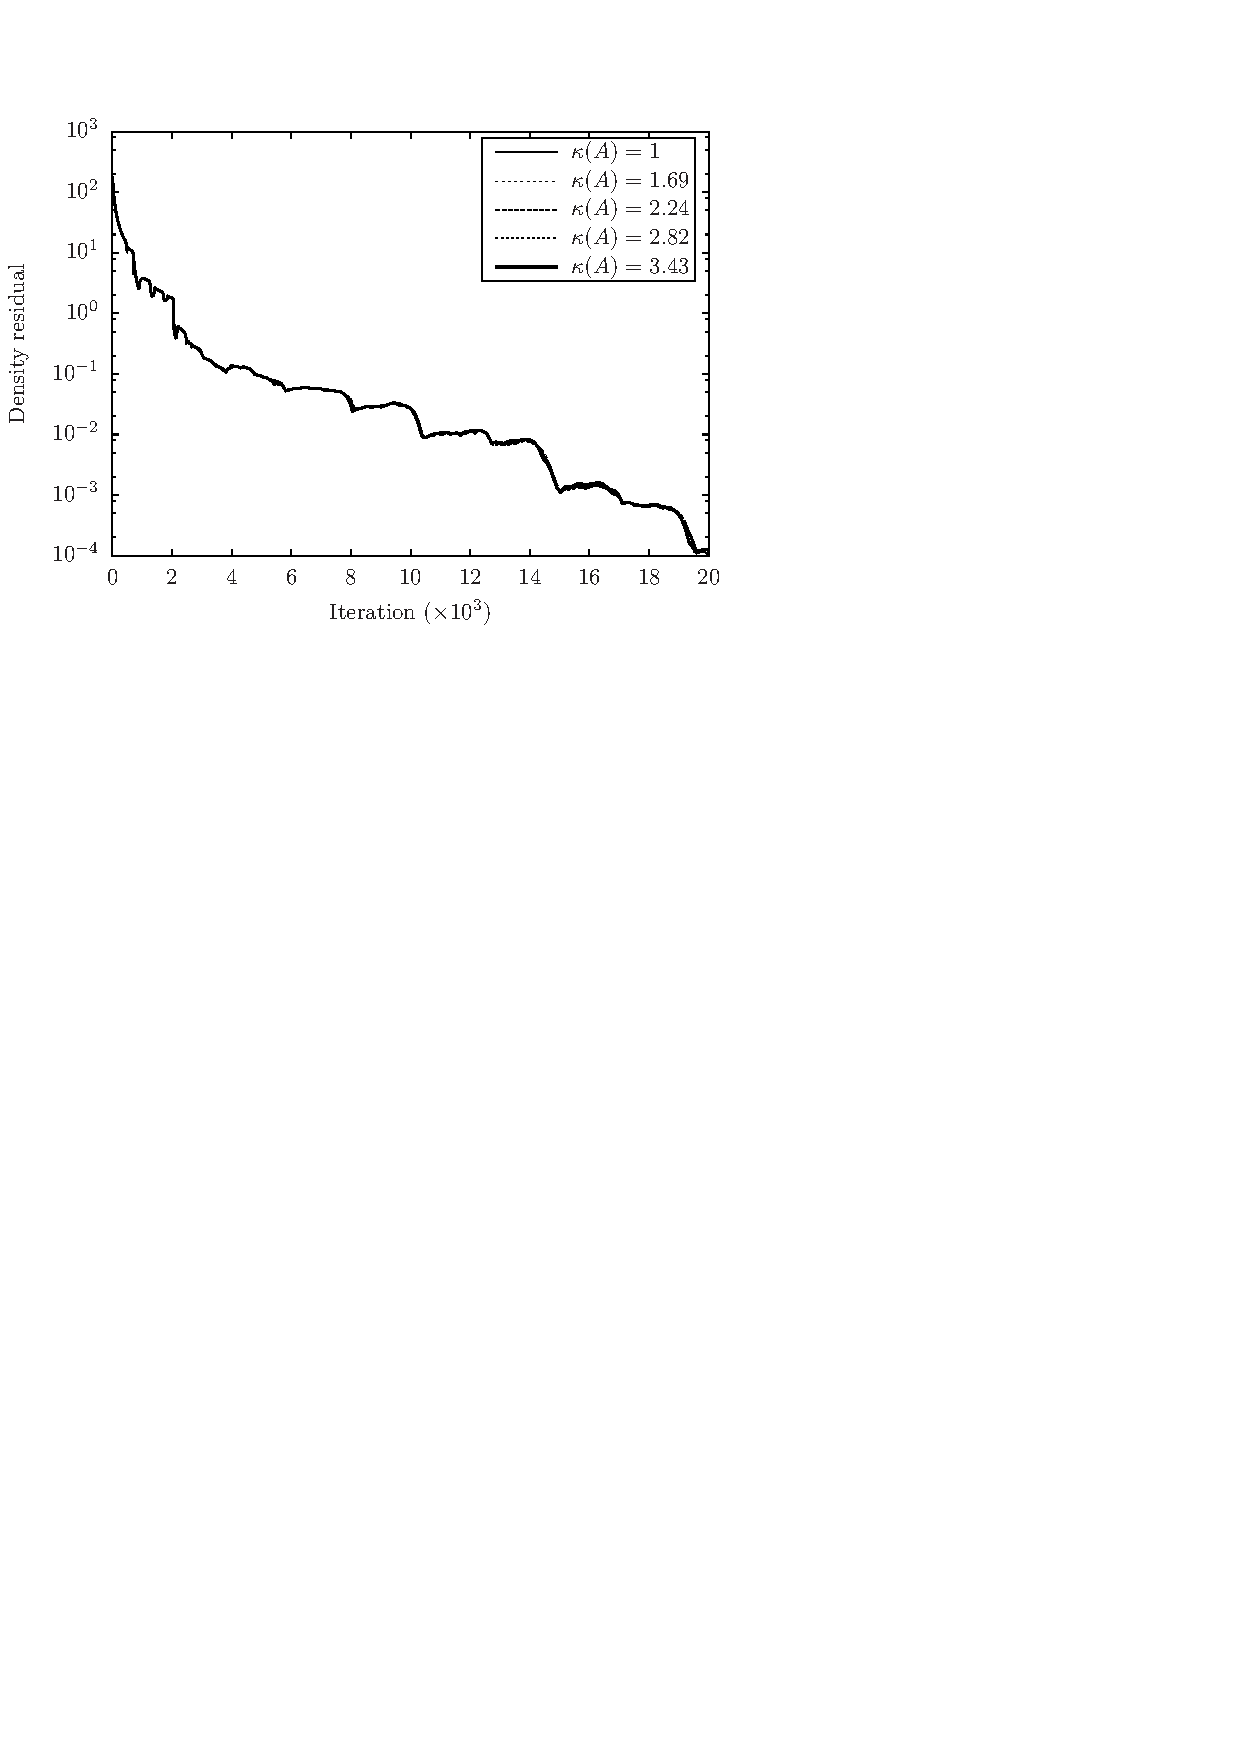
\includegraphics[width=.45\textwidth]{CANAL2_RESIDUAL_VS_CONDITIONNING_AMP001.pdf}}
  \quad
  \subfigure[$A_1=0.05$]{\includegraphics[width=.45\textwidth]{CANAL2_RESIDUAL_VS_CONDITIONNING_AMP005.pdf}}
  \caption{Relation between the condition number $\kappa (A)$ and the
    convergence of the solution.}
  \label{fig:canal_residual_vs_conditionning}
\end{figure}

\paragraph{Using the advection equation model problem}
The same pure harmonic signal is used with the advection equation
model problem:
\begin{equation}
   u_0 (t) = u_m \left[ 1 + A_1 sin \left(2 \pi f_1 t\right) \right]
\end{equation}


\subsection{Solution: Algorithm to automatically choose the timelevels} % (fold)
\label{sec:algorithm_to_automatically_choose_the_timelevels}

Two algorithms that automatically choose the time levels in order to
minimize the condition number are presented: first, the Almost
Periodic Fourier Transform (APFT) algorithm, initially proposed in the
 literature for electronics problems, is described, then a gradient-based
optimization algorithm over the condition number (OPT) is presented.

\paragraph{The APFT algorithm}
\label{sec:apft_algorithm}

Based on the work of \citet{Kundert1988} in
electronics, the APFT algorithm has been implemented.  The aim of the
APFT algorithm is to maximize the orthogonality of the almost-periodic
DFT matrix in order to minimize its condition number.  It is based on
the Gram-Schmidt orthogonalization procedure.  First, the greatest
period $1/\min_k(f_k)$ is oversampled with $M$ equally-spaced time
levels, $M\gg2N+1$ being specified by the user and $N$ the number of
frequencies. Considering these time levels, a rectangular
almost-periodic IDFT matrix is built. Noting that every row of this
matrix is a vector, a set of $M$ vectors is obtained, numbered from 0
to $M-1$, and of length $2N+1$. The first vector $V_0$ (corresponding
to $t=0$) is arbitrarily chosen as the first time level and any
component in the direction of $V_0$ is removed from the following
vectors using the Gram-Schmidt formula:
\begin{equation}
   V_s = V_s - \frac{V_0^\top \cdot V_s}{V_0^\top \cdot V_0} V_0, \quad s=1,\cdots,M-1.
   \label{GramSchmidtAlgo}
\end{equation}
The remaining vectors are now orthogonal to $V_0$.  Since the vectors 
initially have the same Euclidean norm, the vector having the largest
norm is the most orthogonal to $V_0$.  It is assigned to $V_1$. The previous
operations are then performed on the $M-2$ remaining vectors using $V_1$
as $V_0$. This process is repeated until the required $2N+1$ vectors
are defined. As a time instant corresponds to a vector, $2N+1$ time levels are obtained, 
which enables the construction of the almost-periodic
DFT matrix. This algorithm is summarized in
Algo.~\ref{alg:algo_APFT}.

\begin{algorithm}[htb]
\caption{The Almost Periodic Fourier Transform Algorithm.}
\label{alg:algo_APFT}
\begin{algorithmic}
\STATE $\omega_{min} \leftarrow min \left( |\omega_k |,\quad 1 \leqslant k \leqslant N \right)$
\FOR{$m \leftarrow 0,\cdots,M-1$}
    \STATE $t_m \leftarrow \displaystyle\frac{2\pi}{\omega_{min}}\frac{m}{M}$
\ENDFOR
\FOR{$n \leftarrow 1,\cdots,2N$}
   \FOR{$m \leftarrow n+1,\cdots,M$}
  \STATE $ V_{m} \leftarrow V_{m} - \displaystyle\frac{V_{n}^\top \cdot V_{m}}{V_{n}^\top \cdot V_{n}} V_{n}$
   \ENDFOR
   \STATE \textbf{argmax()} returns the index of the largest member of a set
   \STATE $k=\textbf{argmax} \left( \| V_s^n \|,\quad n+1\leqslant s \leqslant M\right) $
   \STATE $\textbf{swap}(V_{n+1},V_{k})$
   \STATE $\textbf{swap}(t_{n+1},t_{k})$
\ENDFOR
\STATE $\mathbb{T}_{optimized} \leftarrow [t_0, \cdots, t_{2N}]$
\end{algorithmic}
\end{algorithm}

\paragraph{Gradient-based optimization algorithm (OPT)}
A more direct approach is to seek directly a set of time levels
that minimize the condition number of the associated almost-periodic DFT matrix, 
instead of using orthogonality properties. 
This minimization problem can be solved numerically by 
an optimization algorithm.

The limited memory optimization method of
Broyden-Fletcher-Goldfarb-Shannon (L-BFGS-B, \cite{Byrd1995}) is
used to look for a minimum of the condition number of the
almost-periodic IDFT matrix $\kappa \left(A \left[\mathbb{T} \right]
\right)$ as function of the time levels vector $\mathbb{T}$.  This
quasi-Newton algorithm approximates the inverse Hessian matrix
$H(\kappa \left(A \left[\mathbb{T} \right] \right))^{-1}$ with the
BFGS formula in order to decrease the objective $\kappa \left(A
  \left[\mathbb{T} \right] \right)$ in the direction $-H(\kappa
\left(A \left[\mathbb{T} \right] \right))^{-1}\nabla \kappa \left(A
  \left[\mathbb{T} \right] \right)$.  This descent direction is
associated with the search for a zero of the gradient, which is a
necessary condition for an extrema, in a second order Taylor series.
Finally, a line search on $\alpha$ is performed to minimize $\kappa
\left(A \left[\mathbb{T} - \alpha H(\kappa \left(A \left[\mathbb{T}
      \right] \right))^{-1} \nabla \kappa \left(A \left[\mathbb{T}
      \right] \right) \right] \right)$.  In the present case, the
derivative $\nabla \kappa \left(A \left[\mathbb{T} \right] \right)$ of
the objective with respect to the time levels is approximated by
first-order finite differences.  An open-source implementation of this
reference broadly-used algorithm is
employed~\cite{Nocedal1980}.

Gradient descent methods being local, the L-BFGS-B method converges to a local
minimum of the condition number.  This minimum is unsatisfying if the
starting point $\mathbb{T}$ is not well chosen, therefore a strategy
to find an appropriate one is required.  As shown in the following
comparison, APFT or uniform-sampling time levels do not always
guarantee acceptable condition numbers, and so cannot be used to
provide a starting point for L-BFGS-B. To this aim, the smallest
frequency is uniformly sampled:
\begin{equation}
    \Omega = [\frac{1}{M} \omega_{min}, \ldots, \frac{m+1}{M} \omega_{min}, \ldots, \omega_{min}],
    \label{eq:slitted_period}
\end{equation}
where $M$ denotes the desired number of initial guesses.
This gives a set of periods. Each of them are evenly sampled to obtain a
set of time levels. 
\begin{equation}
    \mathbb{T}_m = \left[ 0, \frac{2 \pi M}{ (2N + 1) (m+1) \omega_{min}}, \ldots, 
                             \frac{2N \pi M}{ (2N + 1) (m+1) \omega_{min}} \right]
    \label{eq:set_of_tlv}
\end{equation}

These time levels sets are then used as initial guesses for the
L-BFGS-B algorithm.

The almost-periodic IDFT matrix is built for
each of these time levels and the corresponding condition numbers are
computed.  A large number $M$, typically thousands, of fractions of the
greatest period gives a large set of potential time levels vectors.
This is acceptable given the very low cost of the computation of the
condition number on such small matrices of size $(2N + 1) \times
(2N+1)$.  From this set, the time levels vector associated with the
almost-periodic IDFT matrix having the smallest condition number is
taken as a starting point.  The optimization algorithm actually achieves
a local adjustment of the time levels.

In this way, the exploitation capability of the gradient-based
optimizer is well combined with the exploration capacity of the
sampling.  This finally gives solutions that are always close to the
ideal value of $1$, as shown in Tab.~\ref{tab:algo_sum}.  The OPT
method is summarized in Algo.~\ref{alg:algo_opt}.
\begin{algorithm}
\caption{The gradient-based optimization algorithm (OPT).}
\label{alg:algo_opt}
\begin{algorithmic}
\STATE $\omega_{min} \leftarrow min \left( |\omega_k |,\quad 1 \leqslant k \leqslant N \right)$
\FOR{$m \leftarrow 0,\cdots,M - 1$}
    \STATE $\omega_m \leftarrow \frac{m + 1}{M} \cdot \omega_{min}$
    \FOR{$i \leftarrow 0,\cdots,2N$}
        \STATE $t_i \leftarrow \displaystyle\frac{i \cdot 2 \pi}{\omega_m \cdot (2N + 1)}$
    \ENDFOR
    \STATE $\mathbb{T}_m \leftarrow [t_0, \cdots, t_i, \cdots, t_{2N}]$
    \STATE $C_m \leftarrow \kappa \left(A \left[\mathbb{T}_m \right] \right)$
\ENDFOR
\STATE \textbf{argmin()} returns the index of the smallest member of a set
\STATE $k \leftarrow \textbf{argmin}\left(C_m,\quad 0\leqslant m \leqslant M-1\right)$
\STATE $\textbf{min\_l-bfgs-b}\left(\kappa \left(A\left[\mathbb{T}\right]\right), \mathbb{T}_{ini}\right)$ returns the optimal 
time levels vector $\mathbb{T}$ with the condition number $\kappa\left(A\left[\mathbb{T}\right]\right)$ as objective function 
using the L-BFGS-B algorithm and  $\mathbb{T}_{ini}$ as starting point.
\STATE $\mathbb{T}_{optimized} \leftarrow 
  \textbf{min\_l-bfgs-b}\left(\kappa\left(A\left[\mathbb{T}\right]\right), \mathbb{T}_{ini}=\mathbb{T}_k\right)$
\end{algorithmic}
\end{algorithm}

\paragraph{Assessment of the algorithms}

Let us consider the case of two frequencies, $f_1$ and $f$. 
Without loss of generality it can be assumed that $f \leq f_1$.
The non-dimensional frequency $\delta_f^*$ is defined as:
\begin{equation}
    \delta_f^* \colon\begin{cases}
        [0: f_1] & \longmapsto[0: 2]\\
        f & \longmapsto 2 \cdot \displaystyle \frac{f_1 - f}{f_1 + f}
    \end{cases}
    \label{eq:delta_f}
\end{equation}
By taking $f_1$ constant, and having $\delta_f^*$ sampled between $0$
and $2$, the whole range of $f \leq f_1$ is explored. Moreover, as
$\delta_f^*$ is anti-symmetric ($\delta_f^*(-f) = - \delta_f^*(f)$), 
and as the almost-periodic IDFT matrix is symmetric $A[-f] = A[f]$, 
the following relation is obtained for the condition number:
\begin{equation}
  \kappa \left(A \left[\delta_f^*\left(-f\right)\right]\right) =
  \kappa \left(A \left[-\delta_f^*\left(f\right)\right]\right) 
  = \kappa \left(A \left[\delta_f^*\left(f\right)\right]\right),
  \label{eq:permutation}
\end{equation}
meaning that the case $f\geq f_1$ can be deduced in a straightforward
way.

For each value of $\delta_f^*$, the condition number of the
almost-periodic IDFT matrix $\kappa ( A )$ is computed, highlighting
the ability of the different algorithms to choose the time levels that
minimize the condition number, for any input frequencies. This
assessment is only valid for two frequencies, but the tendency is similar
when increasing the number of frequencies. Two frequencies are
involved thus five time levels are required. The results of three
algorithms are depicted Fig.~\ref{fig:bench_algo}: (i)~APFT: the
Almost Periodic Fourier Transform algorithm, (ii)~OPT: the
gradient-based optimization algorithm and (iii)~EQUI: evenly spaced
time levels oversampling the largest period as done in
\citet{Gopinath2007} using $2N+1$ time
levels and in \citet{Ekici2007, Ekici2008} using $3N+1$
time levels.
\begin{figure}[htb]
  \centering 
    \subfigure[Evenly-spaced time levels
    algorithms]{\includegraphics[width=.45\textwidth]{NONEQUI_BENCH_EQUI.pdf}}
    \quad\subfigure[Proposed
    algorithms]{\includegraphics[width=.45\textwidth]{NONEQUI_BENCH_ALGO.pdf}}
  \caption{Comparison of the presented algorithms.}
  \label{fig:bench_algo}
\end{figure}

The EQUI algorithms give fair results ($\kappa(A) \leq 2$) only at
discrete points, corresponding to the particular cases where $f$ is a
multiple of $f_1$, which are thus similar to the single-frequency
case. Oversampling improves the results. In fact, the mean condition number obtained
with $20N + 1$ time levels indicates that the higher the number of time levels
the better the condition number. However the almost-periodic DFT
matrix becomes rectangular and the memory cost of such a computation
increases drastically, preventing the use of such an approach on industrial cases. The APFT
algorithm improves the results, as it gives results with $\kappa ( A
)$ close to unity for $0.3 \leq \delta_f^* \leq 1.2$. However, when
$\delta_f^*$ tends to the boundaries (0 and~2), the condition
number seems to go to infinity. This corresponds to special values
of~$f$:
\begin{equation}
  \begin{split}
    \delta_f^* = 0 & \iff f = f_1, \\
    \delta_f^* = 2 & \iff f = 0. \\
  \end{split}
  \label{eq:singularities}
\end{equation}
This means that the APFT algorithm fails to work when the frequencies
are too close to one another, and when they are significantly
different.  This limits the method for a range of frequencies where
the HB method could give a salient gain in CPU time.
Finally, the OPT algorithm gives a condition number close to unity for
any value of $\delta_f^*$. The OPT algorithm thus ensures that the
convergence of the HB method is not sensitive to the specified set of
frequencies. Table~\ref{tab:algo_sum} summarizes the results obtained
with each algorithm.
\begin{table}[htb]
  \centering
  \begin{tabular}{|r|*{5}{c|}}
    \hline
    & \multicolumn{3}{c|}{EQUI} & APFT & OPT\\
    \hline
    \# instants & $2N+1$ & $3N+1$ & $20N+1$ & $2N+1$ & $2N+1$ \\
    \hline
    \hline
    $\min \left( \kappa \left[A\right]\right) $ & $1.002$ & $1.0$ & $1.0$ & $1.001$ & $1.000$ \\
    \hline
    $\max \left( \kappa \left[A\right]\right) $ & $3.024\cdot 10^{14}$ & $1.871\cdot 10^{11}$ & $2732.6$ & $823.8$ & $2.905$ \\
    \hline
    $\textrm{mean} \left( \kappa \left[A\right]\right) $ & $3.081\cdot 10^{11}$ & $1.871\cdot 10^{8}$ & $10.92$ & $7.742$ & $1.097$ \\
    \hline
  \end{tabular}
\caption{Global results for the presented algorithms.}
\label{tab:algo_sum}
\end{table} 

Thus the proposed non-uniform time sampling combined with the OPT
algorithm allows to tackle problems with large frequency
separation. In such cases, the gain of the HB approach compared
to classical time-marching methods is expected to be significant: with
a time-marching scheme, the time-step has to be small enough to
discretize the shortest period, while the number of time steps of the
simulation has to be long enough to reach the (almost-)periodic state
(\emph{i.e.}  the simulation time is equal to several
times the longest period). Conversely, the cost of the HB method only
depends on the number of frequencies to capture, regardless of their
relative values.

\paragraph{Distribution of the time levels}

For harmonically-related frequencies, the optimal time levels
correspond to a uniform set sampling the fundamental frequency period
as it gives the theoretical lower bound $\kappa (A) = 1$. Since the
frequencies are harmonically related, the distribution of the time
levels on the other frequencies is also uniform. Considering the
frequency vector $F = \left[f_1, \cdots,f_k= kf_1,\ldots,Nf_1 \right]$
and the time levels vector
$\mathbb{T}$:% evenly spaced on the first harmonic period:
\begin{equation}
  \mathbb{T} = \left[0, \frac{1}{f_1\cdot(2N+1)}, \cdots,  \frac{2N}{f_1\cdot(2N+1)} \right],
  \label{eq:evenly_spaced_timelevels}
\end{equation}
then the product of the $i^{th}$ term of $\mathbb{T}$ to its
associated frequency is
\begin{equation}
  f_1 \cdot \frac{i}{f_1\cdot(2N+1)} = k f_1 \cdot \frac{i}{k f_1 \cdot (2N+1)} = f_k \cdot \frac{i}{f_k\cdot(2N+1)}.
  \label{eq:evenly_spaced_timelevels_2}
\end{equation}
Eq.~\eqref{eq:evenly_spaced_timelevels_2} means that evenly-spaced
time levels for the fundamental frequency are still seen as evenly
spaced by the $k^{th}$ harmonic. This is an explanation why the
condition number of the almost-periodic IDFT matrix $A^{-1}$ will be
unity as each frequency is sampled by evenly spaced time
levels~\cite{Brambilla1999}.

Now, considering non-harmonically related frequencies, there is
mathematically no reason for evenly-spaced time levels over the
smallest frequency to be seen as evenly spaced by the other frequencies
in general. Therefore, the use of non-evenly spaced time levels,
  and algorithms to automatically choose them, becomes necessary.

Figure~\ref{fig:distribution_tlv} shows the distribution of the time
levels, relative to each frequency period, obtained by the presented
algorithms for the frequencies $f_1 = 3$~Hz and $f_2 = 17$~Hz (\emph{i.e.}
$\delta_f^*=1.4$).  To do so, the chosen time levels are redistributed
on the considered frequency period by applying a modulo to it:
\begin{equation}
  \label{eq:1}
  \mathbb{T}^{[f_k]}_j =  \mathbb{T}_j \text{ modulo } 1/f_k
\end{equation}
Then, they are divided by the latter, so that the results are
dimensionless.  In light gray line is depicted the $y=x$ function
representing the evenly-spaced solution on the considered period.
Keeping in mind that if each frequency sees evenly-spaced time levels,
then the condition number is the smallest, the optimal solution would
be to have relative time levels on $y=x$ for each period.  Running the
EQUI, APFT and OPT algorithms leads to a condition number of $33.1$,
$3.8$ and $1.1$, respectively.  The EQUI algorithm is perfect for the
period $1/f_1$ but is really far from the evenly spaced time levels
for period $1/f_2$. The APFT algorithm is far from the evenly spaced
solution for both the periods considered, but closer than EQUI regarding
period $1/f_2$. Finally, the OPT algorithm is the only one to be close
to the evenly spaced solution for each considered period, allowing 
the proposed HB method to be used for any set of frequencies.
\begin{figure}[htb]
  \centering \subfigure[Relative to period
  $1/f_1$]{\includegraphics[width=.45\textwidth]{NONEQUI_TIMELEVELS_POSITION_F1.pdf}}
  \quad\subfigure[Relative to period
  $1/f_2$]{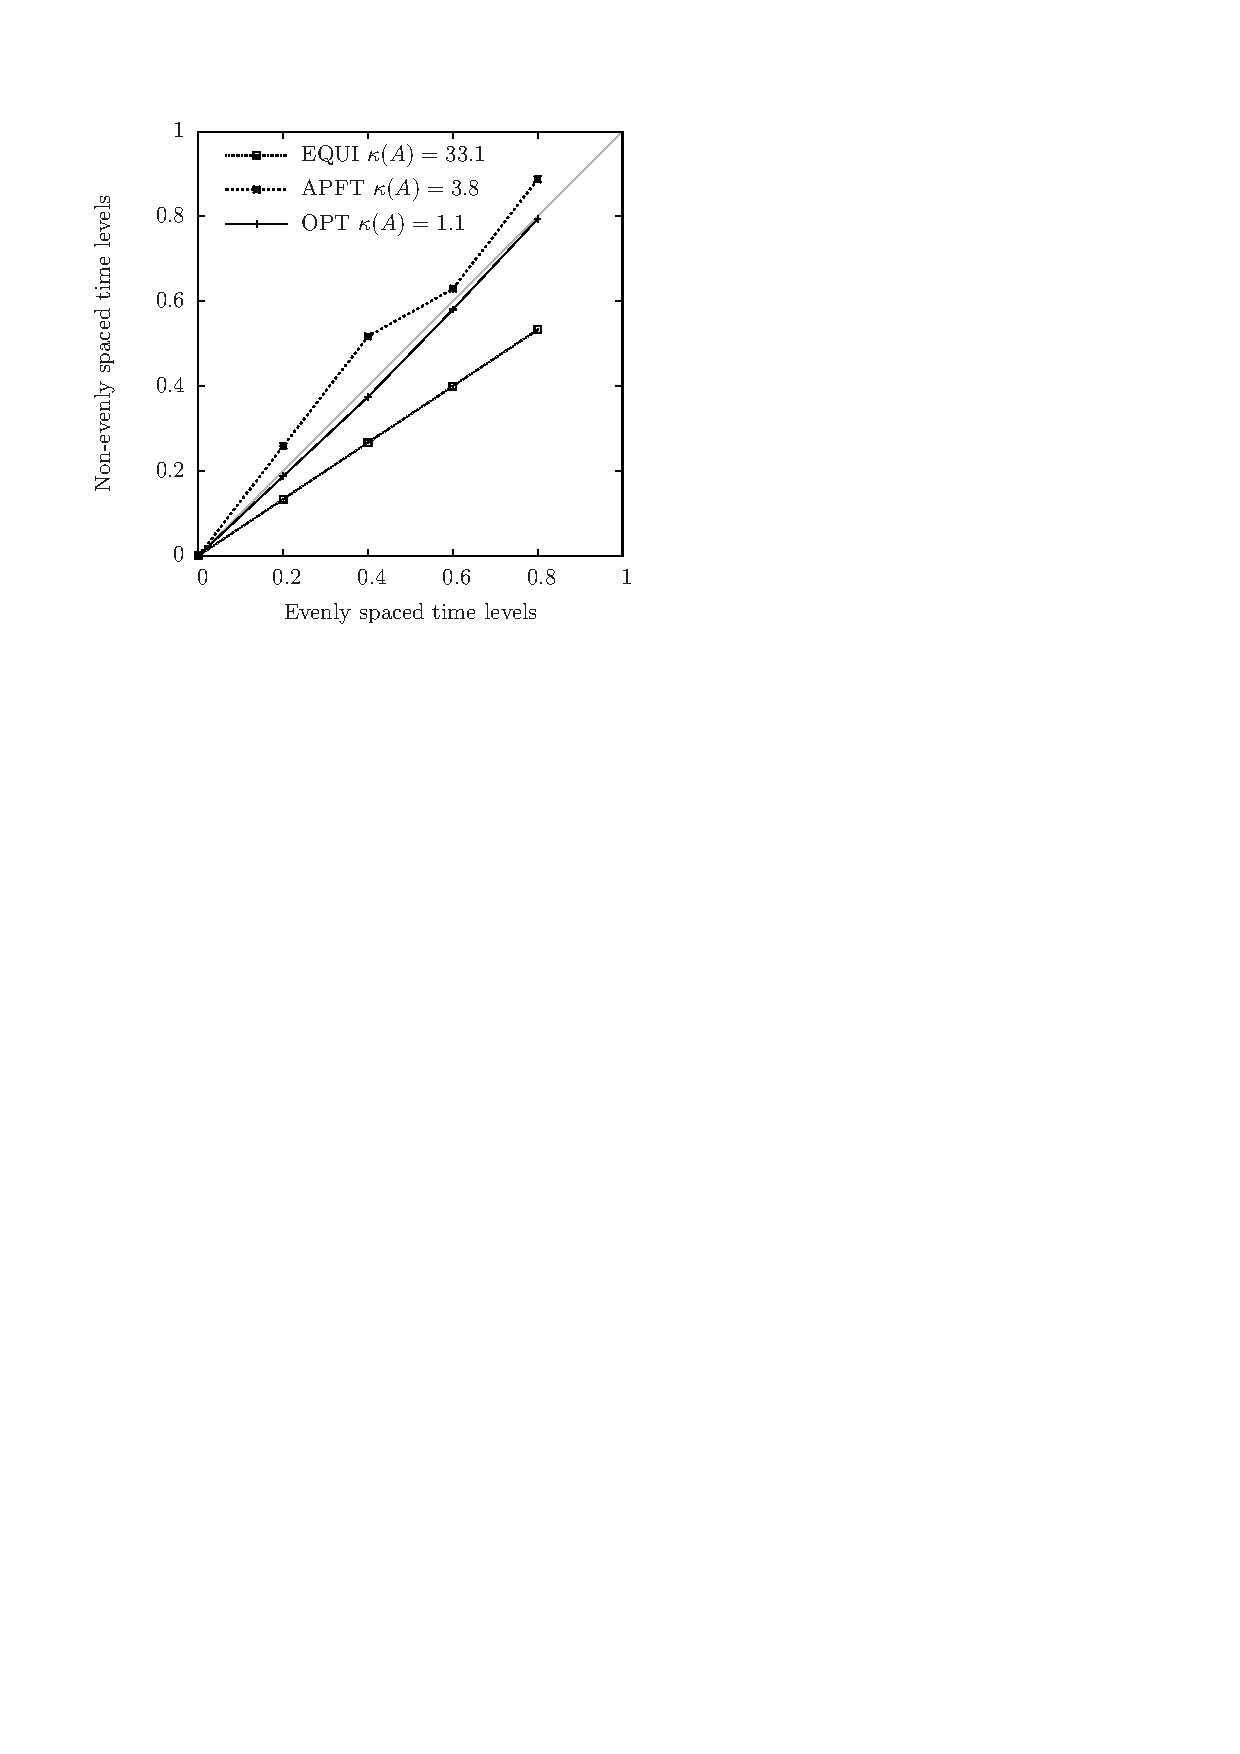
\includegraphics[width=.45\textwidth]{NONEQUI_TIMELEVELS_POSITION_F2.pdf}}
  \caption{Distribution of the time levels on each frequency periods.}
  \label{fig:distribution_tlv}
\end{figure}

The source code of the proposed algorithms and the scripts to generate
Figures~\ref{fig:bench_algo} and~\ref{fig:distribution_tlv} are available
over the internet\,\footnote{\url{http://cerfacs.fr/~gomar/PyLeap.html}}.

The impact of the time sampling on HB computations is now investigated
for the simple case of a channel flow with fluctuating pressure
outlet.


\section{Convergence for turbomachinery computations}
\label{sec:lim_convergence}
%!TEX root = ../../../adrien_gomar_phd.tex


\subsection{Highlighting the problem}

\paragraph{Rectangular function}

In fluid dynamics, the simplest model 
representative of a shock wave
is the step function.
In fact, in a
shock, the variables present a discontinuity
that can be, at first order, represented by a 
step function. In this study, we will consider for periodicity reasons,
the symmetric version of the step function which is the
rectangular function defined as:
\begin{equation}
    u_0(t) = 
    \begin{cases}
        0, & \text{if } 0 \leq t < \frac{T}{2} \\
        1, & \text{if } \frac{T}{2} \leq t < T.
    \end{cases}
    \label{eq:inject_step}
\end{equation}
The rectangular function is periodized using Eq.~\eqref{eq:periodic_operator}.
% as explained above, since
% it is not periodic in essence.

\begin{figure}[htbp]
  \centering
  \subfigure[$N=1$ computation]{\includegraphics[width=.4\textwidth]{convection_step_N1.pdf}}
  \subfigure[$N=2$ computation]{\includegraphics[width=.4\textwidth]{convection_step_N2.pdf}}
  \subfigure[$N=3$ computation]{\includegraphics[width=.4\textwidth]{convection_step_N3.pdf}}
  \subfigure[$N=4$ computation]{\includegraphics[width=.4\textwidth]{convection_step_N4.pdf}}
  \subfigure[$N=5$ computation]{\includegraphics[width=.4\textwidth]{convection_step_N5.pdf}}
  \subfigure[$N=6$ computation]{\includegraphics[width=.4\textwidth]{convection_step_N6.pdf}}
  \caption{Harmonic balance results for 
  an injected rectangular function.}
  \label{fig:inj_step_results}
\end{figure}

Figure~\ref{fig:inj_step_results} depicts the harmonic balance
computations from $1$ to $6$ harmonics. The convergence rate 
is slow as for the $N=6$ harmonics computation, the
shape of the rectangular function is still barely captured. 
In fact, the discontinuity is badly captured and a lot of low
oscillations remains. A Gibbs
phenomenon~\cite{gibbs} is also observed which is in agreement with 
the use of Fourier-based methods to capture a discontinuity. This has been
previously observed by Hembera et al.~\cite{Hembera2009} using
another Fourier-based method, namely the Non-Linear 
Harmonic (NLH) approach~\cite{He1998}.


\begin{figure}[htbp]
  \centering
  \includegraphics[width=.5\textwidth]{convection_step_error.pdf}
  \caption{Convergence of the harmonic computations for an injected
    rectangular function.}
  \label{fig:conv_step}
\end{figure}
As for the previous sum of sine functions, the $\mathcal{L}_2$-norm 
of the error is depicted in Fig.~\ref{fig:conv_step}. 
The convergence of the sum of sine functions is added for comparison.
The convergence rate is different from the previous one: no threshold phenomenon
is seen, the convergence is monotonic and slow.

To further analyze the convergence, 
the discrete Fourier transform of the results
is computed and depicted against analytical result in Fig.~\ref{fig:dft_step}.
The analytical discrete Fourier transform has
 a cardinal sine shape discrete Fourier transform.
\begin{figure}[htbp]
  \centering
  \includegraphics[width=.5\textwidth]{convection_step_dft.pdf}
  \caption{Discrete Fourier transform of the computational
  results compared to the analytical one for an injected 
  rectangular function.}
  \label{fig:dft_step}
\end{figure}
Again, the more harmonics in the computation, the closer the solution
to the analytical results. Surprisingly, only the odd harmonics are
correctly captured while the even ones converge slowly. This might be an
effect due to the shape of the function that is computed. Actually, the odd
sine functions are correctly capturing the shape of the rectangular function, 
as the slope is properly oriented for each stepping part.
\begin{figure}[htbp]
  \centering
  \subfigure[first harmonic]{\includegraphics[width=.3\textwidth]{STEP_ODD_EVEN_1.pdf}}
  \subfigure[second harmonic]{\includegraphics[width=.3\textwidth]{STEP_ODD_EVEN_2.pdf}}
  \subfigure[third harmonic]{\includegraphics[width=.3\textwidth]{STEP_ODD_EVEN_3.pdf}}
  \caption{Capturing a rectangular function with sine functions.}
  \label{fig:step_conv_sine}
\end{figure}
In Fig.~\ref{fig:step_conv_sine} is depicted the convergence of each harmonic
of a sine decomposition for a rectangular function. 
The derivative of the function is better 
handled by odd sine function than even ones. 
This roughly means that introducing an even sin function
damages the solution.
This explains
why the analytical Fourier transform shows small amplitudes for even harmonics.
However this does not explains why even harmonics converges slowly
in Fig.~\ref{fig:dft_step}. For unresolved computations, as these ones for
instance, the convergence is hard to explain. It looks like some harmonics
retrieve a part of the energy that is not computed since they are
filtered by the Fourier-based method. This behavior was also seen on the
previous case.
Again, the convergence of the computations seems
to follow the shape of the analytical solution as when the number
of harmonics grows, the Fourier transform of the results gets closer
to the analytical Fourier transform.

Let us clarify one important thing here: Fourier-based methods
will show Gibbs phenomenon only if a discontinuity is temporally
present. In fact, Fourier-based methods act on the temporal discretization
term, any other term being solved in the classical manner. 
This effect can be emphasized by two 
aero-elastic computations that have been performed 
using an harmonic
balance approach. The first one is the case of 
an airfoil with an oscillating 
flap~\cite{JDufour2010}. In this simulation, as the flap is oscillating
under transonic inflow conditions, a shock swings temporally
back and forth from the pressure side to the
suction side and vice versa. As the discontinuity is
both spatial (a shock is seen on the field) and temporal
(this shock is moving with respect to the time), the number
of harmonics needed to capture this phenomenon is
consistent with the capturing of a rectangular function.
Contrarily, two recent publications~\cite{Huang2013,JSicot2012} on the validation
of the use of harmonic balance approach to predict
aero-elasticity damping within turbomachineries, have highlighted
different conclusions. The 11~\textsuperscript{th}
Standard Configuration~\cite{Fransson1999} for aero-elasticity is computed
for validation in both publications. The transonic case
of this configuration shows a passage shock. Under the first bending mode
of the blade, the shock does not oscillate relative to the blade
movement. As the shock
is only spatial, both publications show a convergence of 
Fourier-based methods with only $N=1$ harmonic. Thus, if the shock
structure is only spatial, Fourier-based methods will not need
extra harmonics to converge, while for a temporally moving discontinuity
(which is the case of our rectangular function), the number
of harmonics to converge will be higher.

Since the present paper focuses on the convergence of turbomachinery
computations, the wake of a blade will be first
simplified and the convergence of harmonic computations will then be
explained.

\paragraph{Towards a turbomachinery wake}
\label{sec:turbomachine_wake}

Consider for generality a stage of a turbomachinery composed of two rotors
with a relative speed difference between the two rows.
Due to the boundary layer that develops on 
the pressure side and the suction side of the blades, a wake is generated behind
the upstream and the downstream rotor. It is stationary in its frame of reference.
\begin{figure}[htb]
    \centering\includegraphics[width=.45\textwidth]{TURBOMACHINES_WAKE.pdf}
  \caption{Characteristic rotor-rotor configuration of a turbomachinery. 
  Wakes are depicted with dashed lines.}
  \label{fig:rotor-stator}
\end{figure}
However, when it crosses the rotor-rotor interface,
the wake becomes unsteady in the downstream rotor frame of reference
because of their relative speed difference. Thus, 
an upstream steady azimuthal heterogeneity becomes unsteady in
the downstream row.

In their pioneer work, 
Lakshminarayana and Davino~\cite{Lakshminarayana1980} showed that the wake
in a turbomachinery follows a similarity law for the velocity. 
It can be statistically estimated by a Gaussian function:
\begin{equation}
    u (\theta) = u_m - 
        \Delta u \cdot e^{
          -0.693 \left( 2 \frac{\theta}{L} \right) ^ 2},
    \label{eq:similarity}
\end{equation}
where $u_m$ denotes the free-stream velocity, $\Delta u$ the axial wake velocity deficit,
$\theta$ the tangential coordinate and $L$ the wake width,
defined as the full width at half maximum.

From the above similarity law and the aforementioned remark on 
the wake becoming unsteady in the downstream row, one can say at 
first order, that the unsteady wake seen by an observer in the downstream row
of reference can be associated with the convection of a periodic 
Gaussian function. The downstream row can be a stator or a rotor,
this holds true for the upstream row. The only condition needed for
this statement to be true, is that a relative motion exists
between the two rows.

The previous convection model problem is now tested
with an injected Gaussian function as defined in Eq.~\eqref{eq:similarity}.
The width $L$ is set to $10\%$ of the domain size $L_x$, 
$u_m$ is set to $1~L_x / c$ and $\Delta u$ to $10\%$ of $u_m$.

\begin{figure}[htbp]
  \centering
  \subfigure[$N=1$ computation]{\includegraphics[width=.4\textwidth]{convection_wake_N1.pdf}}
  \subfigure[$N=2$ computation]{\includegraphics[width=.4\textwidth]{convection_wake_N2.pdf}}
  \subfigure[$N=3$ computation]{\includegraphics[width=.4\textwidth]{convection_wake_N3.pdf}}
  \subfigure[$N=4$ computation]{\includegraphics[width=.4\textwidth]{convection_wake_N4.pdf}}
  \subfigure[$N=5$ computation]{\includegraphics[width=.4\textwidth]{convection_wake_N5.pdf}}
  \subfigure[$N=6$ computation]{\includegraphics[width=.4\textwidth]{convection_wake_N6.pdf}}
  \caption{Harmonic balance results for 
  an injected Gaussian function representing a turbomachinery wake.}
  \label{fig:inj_wake_results}
\end{figure}
Figure~\ref{fig:inj_wake_results} depicts the harmonic balance
computations from $1$ to $6$ harmonics. The convergence toward
the Gaussian function is monotonic and is almost reached
for $N=6$ harmonics. When the number of harmonics is
too small, the width and the depth of the wake are badly estimated
by the method. Moreover, some slight oscillations outside the wake
can be observed, and these disappear along with the growth of the
number of harmonics.

\begin{figure}[htbp]
  \centering
  \includegraphics[width=.5\textwidth]{convection_wake_error.pdf}
  \caption{Convergence of the harmonic computations 
  for an injected Gaussian function representing a turbomachinery wake.}
  \label{fig:conv_wake}
\end{figure}
Figure~\ref{fig:conv_wake} shows the quantitative convergence of 
the harmonic balance computations for a Gaussian function. The
convergence for the two functions studied above are recalled
for comparison.
The convergence rate seams to follow an exponential function
and hence be better than the convergence of the rectangular function.
\begin{figure}[htbp]
  \centering
  \includegraphics[width=.5\textwidth]{convection_wake_dft.pdf}
  \caption{Discrete Fourier transform of the computational
  results compared to the analytical one for an injected 
  Gaussian function.}
  \label{fig:dft_wake}
\end{figure}
The discrete Fourier transform of the results is
depicted against analytical result in Fig.~\ref{fig:dft_wake}.
The $N=2$ and $N=4$ computations badly capture their frequencies.
Starting from the  $N=6$ computation, some of the lower 
frequencies are correctly captured, the last harmonics being
always under-estimated.
Again, adding more harmonics to the harmonic balance
computations greatly improves the resolution of the
modes.

From the previous sections, one can conclude that for
Fourier-Based methods computations, no order
of convergence stands out. The convergence rate follows the decrease
of the spectrum of the temporal signal considered.
This can be named a spectral convergence.

Below some analytical considerations will help us
define a truncation error for the case of wake capturing.

\paragraph{Mathematical analysis of the Gaussian wake model}
\label{sec:analytical_considerations}

The Fourier transform of a Gaussian function is a Gaussian function itself.
If $g$ is a Gaussian function defined as:
\begin{equation}
    g(x) = A e^{-\alpha x^2},
    \label{eq:simple_gaussian_function}
\end{equation}
where $A$ and $\alpha$ are constants, then its Fourier transform is:
\begin{equation}
    \mathcal{F} [g(x)] = \mathcal{F} \left[A e^{-\alpha x^2} \right] = 
    A \sqrt{\frac{\pi}{\alpha}}
      e^{\frac{- \left( \pi f \right)^2}{\alpha}} = \widehat{g}(f),
    \label{eq:fourier_transform_gaussian}
\end{equation}
where $\mathcal{F}$ denotes the Fourier transform operator and $f$ the 
frequency.
$\widehat{g}$ can then be re-written as a classical Gaussian function:
\begin{equation}
    \widehat{g}(f) = A^\prime e^{-\alpha^\prime f^2},
    \label{eq:simple_gaussian_function_spectre}
\end{equation}
where:
\begin{equation}
  \begin{cases}
    A^\prime=A \sqrt{\frac{\pi}{\alpha}}\\
    \alpha^\prime = \frac{\pi^2}{\alpha}.
  \end{cases}
\end{equation}
The exponential factor of the wake law~$\alpha$ is inversely
proportional to its Fourier counter-part~$\alpha'$, meaning that their
width will vary in opposite way: the wider the wake, the thinner its
spectrum and vice-versa.

For the similarity law of Lakshminarayana and Davino, $\alpha$ and $\alpha^\prime$ can be identified:
\begin{equation}
    \alpha =  0.693 \left( \frac{2}{L} \right)^2, \quad
    \alpha^\prime =  \frac{1}{0.693} \left( \frac{\pi L}{2} \right)^2.
    \label{eq:gaussian_params_laksh}
\end{equation}

We have proven above that the convergence rate is inherently linked to
the spectrum of the considered unsteady signal.
As the spectrum of the wake is analytical here, one
way to define the theoretical truncation error is to consider 
the energy contained in the unresolved 
part of the spectrum divided by the energy of the full spectrum:
\begin{equation}
    \varepsilon_{th}(f) = \sqrt{\frac{
        \int_f^\infty | \widehat{g}(\zeta)|^2 d \zeta
      }{
        \int_0^\infty | \widehat{g}(\zeta)|^2 d \zeta
      }}.
    \label{eq:def_truncation_error}
\end{equation}
Introducing the error function defined as
\begin{equation}
    \erf(x) = \frac{2}{\sqrt{\pi}} \int_0^x e^{-t^2} dt,
\end{equation}
and the complementary error function defined as
\begin{equation}
    \erfc(x) = 1 - \erf(x) = \frac{2}{\sqrt{\pi}} \int_x^\infty e^{-t^2} dt,
\end{equation}
then
\begin{align}
    \int_0^\infty | \widehat{g}(\zeta)|^2 d \zeta 
    &= \frac{1}{2} \int_{- \infty}^\infty | \widehat{g}(\zeta)|^2 d \zeta \\
    &= \frac{A^{\prime 2}}{2} \sqrt{\frac{\pi}{2 \alpha^\prime}},
\end{align}
and
\begin{equation}
    \int_f^\infty | \widehat{g}(\zeta)|^2 d \zeta = 
      \frac{A^{\prime 2}}{2} \sqrt{\frac{\pi}{2 \alpha^\prime}} \erfc (\sqrt{2 \alpha^\prime} f).
\end{equation}

The theoretical truncation error can then be written as:
\begin{equation}
    \varepsilon_{th}(f) = \sqrt{\erfc (\sqrt{2 \alpha^\prime} f)}.
    \label{eq:analytical_conv}
\end{equation}
One can notice from Eq.~\eqref{eq:analytical_conv} that the 
truncation error does not depend on the wake deficit.

\begin{figure}[htb]
  \begin{center}
    \includegraphics[width=.85\textwidth]{ANALYTICAL_ERROR_PPT.pdf}
  \end{center}
  \caption{Theoretical truncation error of the Lakshminarayana and Davino wake law.}
  \label{fig:analytic_error_paper}
\end{figure}
Eq.~\eqref{eq:analytical_conv} is depicted in
Fig.~\ref{fig:analytic_error_paper}. 
It can be seen that the wider the spectrum,
the higher the number of harmonics needed to
have a certain level of error. 
Moreover, for a thin wake width ($2 \%$ of the pitch)
the number of harmonics required to capture it with a truncation 
error of $10\%$ is up to $25$ harmonics
which states the limit for Fourier-based methods efficiency.
This figure is analytical meaning that it can give an idea
of the number of harmonics required to compute a wake of a given width.
In the previous section, the wake analyzed had a width
of $10\%$. According to the analytical Eq.~\eqref{eq:analytical_conv},
a $10\%$ error is achieve by using $N=7$ harmonics.

The next section details the convergence obtained with Fourier-based methods
on a reduce order problem: two rotating blocks are considered with
a Lakshminarayana and Davino wake injection.

\section{Solution: towards a prediction tool}
\label{sec:CROR}

Originally, this study has been done to understand the convergence
issues seen on Contra-Rotating Open Rotors (CROR) configurations.
In contrast to turbomachinery applications, convergence
in terms of harmonics has been observed to be
slow on some configurations. For instance, computations
made on the \aipx CROR
are still not converged at $N=10$ harmonics.
Conversely, convergence is obtained at $N=7$ harmonics
for the \mockup configuration at high-speed as shown in
Fig.~\ref{fig:cptsm}.
\begin{figure}[htb]
  \centering
  \subfigure[high-speed \aipx computed with $N=10$ harmonics]{
    \includegraphics[width=.4\textwidth]{aipx7_entropy_r75_N10.jpg}
    \label{fig:cptsm_1}}\quad
  \subfigure[high-speed \mockup computed with $N=7$ harmonics]{
    \includegraphics[width=.4\textwidth]{DREAM_HS_TSM_N7_roe3_sa_slice_r_75_entropy_BW.png}
    \label{fig:cptsm_2}}
  \caption{Entropy field of harmonic balance computation 
  for two CROR configurations at $75\%$ relative span.}
  \label{fig:cptsm}
\end{figure}
To investigate this issue, three configurations are studied:
\begin{itemize}
  \item the \aipx CROR 
  at high-speed (or cruise) condition
  and flight level (\emph{i.e.}  $P_i=23,842$~Pa and $T_i=219.6$~K),
  \item the \mockup CROR at low and high-speed conditions
  but at ground level (\emph{i.e.} $P_i=101,300$~Pa and
  $T_i=293$~K). In fact, these two cases were prone to 
  experimental investigations, hence the ground level.
\end{itemize}
Initially, it has been discovered that adding more harmonics in
the HB computations results in the improvement
of the capture of the wake.
Fig.~\ref{fig:crorroxvmap} shows the
axial momentum taken at the rotor/rotor interface
for the three considered configurations. These are extracted
from an affordable mixing-plane computation~\cite{Denton1979}.
It can be seen that, upstream the rotor-rotor interface,
the main tangential distortion seen is the wake. 
This is true for 
a relative span between $10\%$ and $90\%$, where $0\%$ corresponds
to the hub and $100\%$ the blade tip. 
For higher relative span, the distortion that is seen
is attributed to the tip-vortex, while smaller
relative span highlights viscosity effects near the hub.
One can observe different wake shapes. The High-Speed (HS) \aipx wake looks much
thinner than the HS \mockup which also looks
thinner than the Low-Speed (LS) one. Indeed, the latter does not show a
well delimited wake structure all along the span.
\begin{figure}[htbp]
  \centering
  \subfigure[\mockup -- low speed]{\includegraphics[width=.32\textwidth]{dream_ls.png}}
  \subfigure[\mockup -- high speed]{\includegraphics[width=.32\textwidth]{dream_hs_roe2.png}}
  \subfigure[\aipx -- high speed]{\includegraphics[width=.32\textwidth]{aipx7.png}}
  \caption{Non-dimensional axial momentum $(\rho U)/(\rho U)_\infty$ 
  upstream the rotor/rotor interface.}
  \label{fig:crorroxvmap}
\end{figure}

\subsection{Wake width criterion}
At first order, one can thus infer that for a relative
span contained between $10\%$ and $90\%$, the main
tangential distortion seen is the wake. 
To estimate the wake thickness, a curve
fitting algorithm is used to fit the Lakshminarayana
and Davino Gaussian wake law. The thickness
of the wake is plotted in Fig.~\ref{fig:crorwakethick_a}.
\begin{figure}[htbp]
  \centering
  \subfigure[Thickness estimation]{
  \label{fig:crorwakethick_a}
  \includegraphics[width=.45\textwidth]{CROR_THICKNESS.pdf}}
  \subfigure[$\mathcal{L}2$-norm for the estimation]{
  \label{fig:crorwakethick_b}\includegraphics[width=.45\textwidth]{CROR_THICKNESS_ERROR.pdf}}
  \caption{Estimation of the relative wake thickness for the three contra-rotating
  open rotor configurations.}
  \label{fig:crorwakethick}
\end{figure}
To assess the quality of the curve fitting
algorithm, the $\mathcal{L}2$-norm
of the error is plotted in Fig.~\ref{fig:crorwakethick_b}.
For all three configurations, the error follows the same trend.
Near the hub (relative span inferior to $10\%$) the error is
maximum. Between $10\%$ and $70\%$ the error increases but
remains relatively low. This is the region
where the main tangential distortion is
actually a wake, hence the good fitting. 
In the tip vortex region (relative
span between $70\%$ and $100\%$), the error increases
and reaches a maximum in the core of the tip vortex.
In this region, the tangential distortion is not a wake
and explains the difficulty of the curve fitting algorithm
to capture a Gaussian function.
Finally, in the far-field region (relative span superior to $100\%$)
the axial momentum decreases toward the infinite velocity, thus
the tangential distortion is a constant field, which explains
the low error.
To qualitatively estimate the level of the curve fitting,
the best (from \mockup HS configuration) and the
worst fits (from \mockup LS CROR) are compared to their
original wake signals in Fig.~\ref{fig:crorwakeestimate}.
For the best fit, the original tangential distortion is
almost superimposed on the equivalent Gaussian wake law, besides
the fact that the wake is not symmetrical. In opposite,
the tangential distortion seen for the worst fit looks like
an inverse Lakshminarayana and Davino wake and does not  
\begin{figure}[htbp]
  \centering
  \subfigure[Best fit]{\includegraphics[width=.45\textwidth]{CROR_WAKE_FITTING_BEST.pdf}}
  \subfigure[Worst fit]{\includegraphics[width=.45\textwidth]{CROR_WAKE_FITTING_WORST.pdf}}
  \caption{Qualitative estimation of the level of the curve fitting for the
  wake in CROR configurations.}
  \label{fig:crorwakeestimate}
\end{figure}
From the error estimate (Fig.~\ref{fig:crorwakethick_b})
and the best/worst fit scenario, one can deduce that
curve fitting works well when the distortion is a wake.
In that case, the thickness estimation is reliable. 

One can thus say that the wake is relatively well-defined
between $10\%$ and $70\%$ relative span. 
It can be seen that the wake of the 
LS \mockup is about $30\%$ of the pitch, the one of the HS
\mockup 
being approximately $10\%$ while the
\aipx wake is thinner as it is around $4\%$ of the pitch.

Based on the
analytical formula derived in Sec.~\ref{sec:analytical_considerations},
if the wake width is known, one can deduce the
number of harmonics needed to capture a wished level of error
$\overline{\varepsilon}$:
\begin{equation}
    N = \frac{\ierfc \left[\overline{\varepsilon}^2 \right]}{
    \sqrt{2 \alpha^\prime}},
    \label{eq:estimation_nb_harms}
\end{equation}
where $N$ is the number of harmonics, $\ierfc$ the inverse 
complementary error function (namely $\erfc^{-1} = \ierfc$),
$\varepsilon$ and $\alpha^\prime$ are the truncation error
and the wake parameter, respectively, as defined in 
Sec.~\ref{sec:analytical_considerations}.
The level of error required 
for a computation to be rigorously converged
is difficult to estimate. 
Instead of using the level of error, 
we will use the
relative accumulated energy $E(f)$ as defined in 
Eq.~\eqref{eq:correspond_E_error}.
It seems reasonable, from an engineering standpoint, to consider
that a $99\%$ accumulation of energy should be a good starting point.
To emphasize that,
the reconstruction of a wake in function of three levels of cumulative
energy $E$ is depicted in Fig.~\ref{fig:level_of_energy}. 
\begin{figure}[htbp]
  \centering
  \includegraphics[width=.5\textwidth]{LEVEL_OF_ENERGY_PAPER.pdf}
  \caption{Reconstructions of a wake depending on
  the energy content kept in the signal.}
  \label{fig:level_of_energy}
\end{figure}
One can see
that a reconstruction using only $50\%$ of the energy
leads to a signal that has neither
the right wake deficit nor its width. Using
$90\%$ and $95\%$ of the energy improves things a little
but is still not satisfactory as large secondary
oscillations remains as long with a bad capture
of the wake deficit.
In opposite, by using $99\%$ of the energy to reconstruct
the signal, some extra
oscillations are seen but 
the wake width and deficit are recovered with less than 
$95\%$ accuracy.
Thus, the $99\%$ energy threshold ensures that the wake
will be correctly transmitted in the opposite row, which is
the prior concern of this paper.
Thus, based on the $99\%$ energy threshold
and the wake width computed
for all the three CROR configurations shown in Fig.~\ref{fig:crorwakethick},
one can estimate the number of harmonics needed to compute such
applications using Eq.~\eqref{eq:estimation_nb_harms}. 
Approximately, the wake width
of the \aipx, the HS \mockup and the LS \mockup is respectively
$4\%$, $10\%$ and $30\%$. 
Using Eq.~\eqref{eq:estimation_nb_harms},
the theoretical estimation of the number of harmonics needed 
to recover $99\%$ of the energy is respectively
$17$, $7$ and $2$. These numbers explain why the 
\aipx configuration is still not converged after $N=10$
harmonics. Moreover, such a computation leads to a
$87\%$ energy signal. Fig.~\ref{fig:level_of_energy}
supports the argument that with this level of energy, the wake
is not properly captured as a $90\%$ energy signal
does not accurately estimate the wake deficit and thickness.

With this approach, one can deduce approximately
the number of harmonics needed to compute such CROR
configurations using Fourier-based methods. The issue is that it is limited to
well defined wakes. If another tangential
distortion is seen at the interface, the present
criterion cannot be used, which limits the current
method. However, as demonstrated in Sec.~\ref{sub:comp_w_analytic},
the analytical error and the error based on an
azimuthal Fourier transform of the distortion
seen just upstream the interface for a mixing-plane
configuration are similar. 


\subsection{Prediction tool based on an azimuthal Fourier transform}
Thus, a more general way to analyze the spectrum in a wake is
to perform an azimuthal Fourier transform at the rows interface
in a mixing-plane computation. The good thing is
that it both encompass the wake analysis done above and also
any tangential disturbances as for instance
the viscosity effects near the hub or the tip vortex.
The steps to do such an analysis are detailed in
Fig.~\ref{fig:criterion_cror}. First the row
interface is extracted from a mixing-plane computation 
(step \textcircled{\small{$1$}}).
The term row is used to show that this can be done
for a CROR configuration and in general any turbomachinery
configuration where a relative speed motion exists at
the row interface.
The axial momentum is then extracted for a large
number of radii spanning the region of interest
(step \textcircled{\small{$2$}}).
In a CROR configuration this is the region with a 
relative span ranging between $0\%$ and $120\%$.
In fact, for higher relative span ($\geq 120\%$), the fluid motion
is not of prior interest as it is the far-field region.
Finally, for each radii, an azimuthal Fourier transform
is performed to obtain the tangential spectrum of the
axial momentum (step \textcircled{\small{$3$}}).
\begin{figure}[htbp]
  \centering
  \includegraphics[width=.6\textwidth]{CRITERION_CROR.pdf}
  \caption{Steps for the prediction tool based on an azimuthal
  Fourier transform of the rotor-rotor interface.}
  \label{fig:criterion_cror}
\end{figure}
The relative cumulative energy is then easily defined as:
\begin{equation}
    E (N) = \frac{\sum_{k=1}^N \left[ \widehat{\rho U}^{\theta} (k) \right]^2}{ 
    \sum_{k=1}^\infty \left[ \widehat{\rho U}^{\theta} (k) \right]^2},
    \label{eq:def_crit_cror}
\end{equation} 
where $\widehat{\rho U}^{\theta}$ denotes the axial momentum spectrum
extracted from the rows interface plane. In Eq.~\eqref{eq:def_crit_cror},
the cumulative energy up to harmonic $N$ is 
compared to the total energy.
Figure~\ref{fig:crorroxvcurves} shows this energy accumulation
harmonics by harmonics for each configuration at four span
positions, namely four radii. The LS
\mockup is the quickest to reach $100\%$ of energy meaning that the
spectrum is narrow. On the opposite, the \aipx configuration accumulate
energy at a slow rate. Its first harmonic often contains less
than $15\%$ of the spectrum energy except for the $90\%$ span,
and the slope is almost linear which
gives a slow convergence rate compared to the \mockup configurations.
\begin{figure}[htbp]
  \centering
  \subfigure[$30\%$ span]{\includegraphics[width=.46\textwidth]{CROR_SPECTRUM_SPAN30.pdf}}\quad
  \subfigure[$50\%$ span]{\includegraphics[width=.46\textwidth]{CROR_SPECTRUM_SPAN50.pdf}}\quad
  \subfigure[$70\%$ span]{\includegraphics[width=.46\textwidth]{CROR_SPECTRUM_SPAN70.pdf}}\quad
  \subfigure[$90\%$ span]{\includegraphics[width=.46\textwidth]{CROR_SPECTRUM_SPAN90.pdf}}\quad
  \caption{Energy accumulation by harmonics at four span positions.}
  \label{fig:crorroxvcurves}
\end{figure}

To have a global insight of the energy contained in the
tangential distortion for all relative span,
the energy accumulation is plotted using a colormap
in Fig.~\ref{fig:crorroxvmapenergy}. This is just
a way to display Fig.~\ref{fig:crorroxvcurves} for all
relative span in one diagram.
Three contour lines are added to ease the
interpretation: $90\%$, $95\%$
and $99\%$, corresponding to a truncation
error of respectively $30\%$, $20\%$ and $10\%$.
\begin{figure}[htbp]
  \centering
  \subfigure[Mock-Up -- Low Speed]{\includegraphics[width=.55\textwidth]{DREAM_LS_RANS_ROE2_SPECTRUM_PPT.pdf}}
  \subfigure[Mock-Up -- High Speed]{\includegraphics[width=.55\textwidth]{DREAM_HS_RANS_ROE2_SPECTRUM_PPT.pdf}}
  \subfigure[AIPX7 -- High Speed]{\includegraphics[width=.55\textwidth]{AIPX7_RANS_SPECTRUM_PPT.pdf}}
  \caption{Energy accumulation by harmonics for all spans.}
  \label{fig:crorroxvmapenergy}
\end{figure}
The results are in good agreement with the criterion
based on the wake thickness. In fact, for a relative
span between $10\%$ and $90\%$, the number of harmonics
needed to have $99\%$ of the energy is $4$, $7$ and $16$
for respectively the \mockup LS, the \mockup HS and the
\aipx configurations. This is close to the $2$, $7$ and
$17$ number of harmonics found using a curve fitting
algorithm and the theoretical error derived in 
Sec.~\ref{sec:analytical_considerations}.

This prediction tool is more accurate as it handles
both wake tangential distortion and also any other
type of distortion. Thus, this tool can be used to predict
the number of harmonics needed to capture a certain
level of energy for any relative span.
Moreover, it does take into account for the
viscosity effects, which is not the case of the criteria
proposed in Sec.~\ref{sec:rotating_blocks}.

\subsection{Effect of the numerical scheme}

As one can expect, the numerical scheme used to
compute the configuration has a direct impact on the tangential
distortion seen at the interface. The wake that is 
generated behind the blades of the upstream row is
convected toward the rotor-rotor interface. Depending on
the dissipation and dispersion properties of the numerical
scheme, the wake will be seen different downstream of the
first rotor. Fig.~\ref{fig:crorroxvmap_scheme} shows the azimuthal 
distortions observed depending on the numerical scheme.
Three different schemes are used: a first order, a second
and a theoretical third order Roe scheme. The shape of the
tangential distortion follows the same trend  for the three
schemes but is different locally.
The width of the wake seems almost doubled between the first order
Roe scheme and the third order Roe scheme. This holds true for the tip
vortex foot-print.
\begin{figure}[htbp]
  \centering
  \subfigure[first order Roe scheme]{\includegraphics[width=.32\textwidth]{dream_hs_roe1.png}}
  \subfigure[second order Roe scheme]{\includegraphics[width=.32\textwidth]{dream_hs_roe2.png}}
  \subfigure[third order Roe scheme]{\includegraphics[width=.32\textwidth]{dream_hs_roe3.png}}
  \caption{Non-dimensional axial momentum $(\rho U)/(\rho U)_\infty$ 
  upstream the rotor/rotor interface.}
  \label{fig:crorroxvmap_scheme}
\end{figure}

As the tangential distortion is seen different, the prediction tool
will lead to different conclusions. Fig.~\ref{fig:crorroxvmapenergy_scheme}
shows the application of the prediction tool for the three
different numerical schemes. The conclusions are that
$N=5$, $N=7$ and $N=10$ harmonics are needed to recover 
$99\%$ of the energy for respectively the first order, the 
second order and the third order schemes. This is scattered,
almost as the three CROR configurations were in 
Fig.~\ref{fig:crorroxvmapenergy}. 
\begin{figure}[htbp]
  \centering
  \subfigure[first order Roe scheme]{\includegraphics[width=.55\textwidth]{DREAM_HS_RANS_ROE1_SPECTRUM_PPT.pdf}}
  \subfigure[second order Roe scheme]{\includegraphics[width=.55\textwidth]{DREAM_HS_RANS_ROE2_SPECTRUM_PPT.pdf}}
  \subfigure[third order Roe scheme]{\includegraphics[width=.55\textwidth]{DREAM_HS_RANS_ROE3_SPECTRUM_PPT.pdf}}
  \caption{Effect of the numerical scheme on the energy 
  accumulation at the interface of the \mockup HS configuration.}
  \label{fig:crorroxvmapenergy_scheme}
\end{figure}

Actually, all the numerical or physical parameters
that may lead to a thickening or narrowing of the
wake will be taken into account by the prediction tool.



\chconclu{}


\part{Applications}
%!TEX root = ../../../adrien_gomar_phd.tex
\chapter{Presentation of the numerical tools}
\label{cha:numericals}

\chabstract{}

\minitoc
\newpage

\section{\emph{elsA} CFD solver}
\label{sec:num_elsa}
%!TEX root = ../../../adrien_gomar_phd.tex

The following applications have been performed using the
\emph{elsA}\footnote{\emph{elsA} stands for \underline{e}nsemble 
\underline{l}ogiciel pour la \underline{s}imulation en 
\underline{A}\'erodynamique} solver~\cite{Cambier2013} initially developed by ONERA in 1997.


\section{Antares post-processing software}
\label{sec:num_antares}
%!TEX root = ../../../adrien_gomar_phd.tex

\label{app:antares}

A large effort is put today on CFD flow solver
to deliver results as fast as possible while
maintaining their fidelity. The future o
However, a CFD result is meaningless
if it is not post-processed. The aim of post-processing is
to transform raw simulation results into a human-understandable
results. 
\begin{figure}
  \centering
  \includegraphics*[width=0.6\textwidth]{antares.pdf}
  \caption{Antares capabilities.}
  \label{fig:antares}
\end{figure}

\section{Implementation of the harmonic balance}
\label{sec:num_hb}
%!TEX root = ../../../adrien_gomar_phd.tex

implicitation
chorochronic
extension to multi-freq

\section{AEL module}
\label{sec:num_ael}
%!TEX root = ../../../adrien_gomar_phd.tex

weak coupling approach
mesh deformation technique

\chconclu{}

%!TEX root = ../../../adrien_gomar_phd.tex
\chapter{11\texorpdfstring{\textsuperscript{th}}{th} standard aeroelastic configuration}
\label{cha:stcf11}

\chabstract{The harmonic balance method along with an aeroelastic 
\replaced{decoupled}{weak-coupling} approach, is applied to
the well-known 11\textsuperscript{th} standard aeroelastic configuration of
\citet{Fransson1999}. It is shown that by using only
one harmonic ($N=1$), the damping curve of both the subsonic
and the transonic operating points are superimposed with
the reference unsteady computation. The agreement
with both the experimental and the numerical data available
is good, justifying the proposed approach. Moreover, a
speed-up of seven is found compared to a classical 
time-marching scheme. This work has been published in
\begin{quote}
	\citetalias{Sicot2014}
\end{quote}}


\newpage

\section{Presentation of the case}
\label{sec:stcf11_presentation}
%!TEX root = ../../../adrien_gomar_phd.tex

For external-flow aeroelasticity, the HB approach has 
been thoroughly validated by \citet{Gopinath2005, Woodgate2009} and \citet{JDufour2009}, 
mostly for the AGARD test cases of \citet{Davis1982}.
Experimental data for turbomachinery aeroelasticity are more scarce: 
the STandard aeroelastic ConFigurations (STCF) experiments 
of \citet{Fransson1999} are the 
reference in this respect, and have been widely used 
to validate different numerical approaches by \citet{Sbardella2001,
Duta2002,Campobasso2003,Cinnella2004} and \citet{Huang2013a} whose
uses a similar harmonic balance approach as the one proposed in
this work.
The experiments
are composed of 11~turbomachinery configurations that have been
thoroughly investigated experimentally in an 
annular test rig at \'Ecole 
Polytechnique F\'ed\'erale de Lausanne.

In particular, the 11\textsuperscript{th} standard configuration is a
turbine stator composed of 20~blades, and tested
in the late 1990's by \citet{Fransson1999}.
The experimental results have been found to be highly reproducible and
therefore suitable for code validation.  Moreover,
two flow regimes are considered, one subsonic and one transonic.
In this respect, the transonic case allows to distinguish
solvers able to capture non-linear unsteady effects. This is why this particular
case is used here, since HB methods are meant to capture non-linear unsteady
features. However, it must be pointed out that LUR approaches have
been validated using the transonic case and show fair agreement with experimental
data~\cite{Sbardella2001, Duta2002,Campobasso2003}.

% geometry presentation
The geometry profile and the results are available over the
internet~\cite{stcf11web}. 
To characterize the two flow regimes, measurements of static and total pressures 
as well as flow angles are done in two planes $e_0$ located $0.3$ axial chord upstream 
of the turbine
blade and $e_1$ located $0.6$ axial chord downstream
as shown in Figure~\ref{fig:stcf11_measurements}.
\begin{figure}[htp]
  \centering
  \includegraphics*[width=0.40\textwidth]{stcf11_measurements.pdf}
  \caption{Position of the measurement planes in the STCF~11 configuration.}
  \label{fig:stcf11_measurements}
\end{figure}
The results are given in terms of
inlet Mach number $M_0$, inlet total pressure $p_{i_0}$, 
inlet flow angle $\beta_0$, outlet isentropic
Mach number $M_{1_{is}}$ and outlet static pressure $p_{s_1}$. 
The isentropic Mach number is the Mach number 
computed if the stagnation pressure was taken constant (without loss)
\begin{equation}
    M_{is} = \sqrt{\frac{2}{\gamma -1}
        \left[\left( \frac{p_{i_0}}{p_s} \right)^{\frac{\gamma - 1}{\gamma}}  
        - 1 \right]},
\end{equation}
where $p_{i_0}$ is the constant total pressure and $p_s$
the local static pressure.
It is actually
one way to interpret the static pressure as a velocity.
The experimental results measured at plane $e_0$
and $e_1$ are given in Tab.~\ref{tab:stcf11_steady_results}. 
These will be used later on to set the boundary conditions 
of the CFD computations. To allow local validation of the steady
flow, the experimental results of 
isentropic Mach number are given at blade wall.
\begin{table}[htp]
  \ra{1.3} \centering
  \begin{tabular}{lccccc}
    \toprule
    \phantom{abdefghijk}& $M_0~[-]$ & $p_{i_0}~[\text{Pa}]$ & $\beta_0~[\circ]$ & $M_{1_{is}}~[-]$ & $p_{s_1}~[\text{Pa}]$ \\
    \midrule
    Subsonic & $0.31$ & $124,600$ & $15.2$ & $0.69$  & $90,700$ \\
    Transonic & $0.4$ & $229,800$ & $34$    & $0.99$ & $122,400$ \\
    \bottomrule
  \end{tabular}
  \caption{Steady experimental results for the STCF~11 configuration.}
  \label{tab:stcf11_steady_results}
\end{table} 

For aeroelastic investigations, the blades oscillate harmonically in the first bending mode
at a reduced frequency of $f_{c} =\pi c f/U_{outlet, exp} = 0.2134$ 
for the subsonic case and $0.1549$ for the
transonic case. Aeroelastic
results are available such as the first harmonic of the unsteady pressure
coefficient at blade walls (amplitude and phase), for several nodal
diameters. These are measured using piezo-resistive pressure transducers.

The damping is evaluated at blade walls through through the
expression given by~\citet{Fransson1999}
\begin{equation}
    \textrm{Damping } [-] = - \sum^{\#~pts}_{k=0} \frac{c}{h} 
      \frac{|\widehat{p}_k|}{(p_{i_0} - p_{s_0})} S_k \arg (\widehat{p}_k),
\end{equation}
where $c$ is the chord length,
$h$ the bending amplitude, $| \widehat{p} |$ 
and $\arg (\widehat{p})$ are the modulus and the phase of the
complex first harmonic of static pressure, respectively, $S$ the surface
and $k$ denotes the k\textsuperscript{th}
grid point at blade walls.
The damping strongly varies under small changes in the
local distribution. It is therefore recommended to look at the local
distributions. No experimental damping curves are given. In fact,
there is too few measurement points to integrate the results with
confidence. However, \citet{Fransson1999}
provide numerical results of the damping curve obtained with a potential code.



\section{Numerical setup}
\label{sec:stcf11_numerical}
%!TEX root = ../../../adrien_gomar_phd.tex

% mesh presentation
The blade passage is meshed using an O4H topology as
shown in Figure~\ref{fig:stcf11_mesh}.
The number of grid points along the blade
chord is~160 and the computed $y^+$ at the walls is $\mathcal{O}(1)$.
81~points are used to discretize the azimuthal direction.
The blade has the same profile along the spanwise direction and no
twist. Therefore, a 2.5D mesh is used with five points 
in the radial direction. The spanwise
extent represents $1\%$ of the chord. 
The total size of the mesh is 70,330.
\begin{figure}[htp]
  \centering
  \includegraphics[width=.46\linewidth]{STCF11_MESH.pdf}
  \caption{STCF 11 mesh.}
  \label{fig:stcf11_mesh}
\end{figure}

% boundary conditions
The \textit{elsA}~\cite{Cambier2013} CFD code 
along with its aeroelastic
module~\cite{CIDugeai2011} is used to solve this configuration.
The boundary conditions used for this case are: (i)~an
injection condition  for the inlet (with the relative flow angle,
the Mach number and the total pressure
set to the experimental values using Tab.~\ref{tab:stcf11_steady_results}), 
(ii)~a constant static pressure
condition for the outlet using also the value $p_{s_1}$
given in Tab.~\ref{tab:stcf11_steady_results},  
(iii)~an adiabatic no-slip condition on
blade walls, and (iv)~periodic or phase-lagged conditions 
for azimuthal boundaries depending on the  
prescribed IBPA.

% numerical parameters
Turbulence is modeled using the one-equation model of
\citet{Spalart1992}.  Roe's scheme~\cite{Roe1981} along with a 
third-order MUSCL extrapolation 
is used to compute the convective fluxes.
The classical Dual Time-Stepping~\cite{Jameson1981} (DTS)
time-integration scheme is taken for comparison to the
proposed harmonic balance approach.
The maximum
CFL number is set to~20 for the steady computations,  the inner loop
of the DTS scheme and the HB simulations.  For the DTS scheme,  
convergence in time discretization is obtained
after 20~periods using 128~time steps per period.  Iterative convergence 
for the inner loop is considered achieved when the normalized
residuals drop by $5\e{-2}$ (within a maximum of
50~sub-iterations).

% The steady and unsteady post-processing is done using the
% Antares post-processing software 
% (Appendix~\ref{app:antares}).

\paragraph{Influence of the mesh discretization}
\label{sub:stcf11_mesh_convergence}
The mesh quality is assessed through a mesh convergence.
To ensure the latter, three meshes are tested, the referenced one
described above, and two meshes, coarse~2 and coarse~4,
coarsened in the axial and
azimuthal directions by a factor of two and four, respectively. 
The five grid points in the radial direction
are kept unchanged.

The steady results for the two operating points are shown 
in Figure~\ref{fig:stcf11_mesh_convergence}.
\begin{figure}[htp]
  \centering
  \subfigure[subsonic]{
    \includegraphics[width=.4\textwidth]{STCF11_RANS_SUBSONIC_CONVERGENCE_MESH_PPT.pdf}}
  \subfigure[transonic]{
    \includegraphics[width=.4\textwidth]{STCF11_RANS_TRANSONIC_CONVERGENCE_MESH_PPT.pdf}}
  \caption{Influence of mesh discretization for the STCF~11 configuration.}
  \label{fig:stcf11_mesh_convergence}
\end{figure}
The three meshes give the same results for the subsonic case. On the
pressure side (bottom curve), the three results are superimposed. On the suction side
(top curve),
some minor differences are observed in particular near the leading edge
($x / c \leq 0.2$). Nevertheless, the agreement
between the three meshes is very good for the subsonic operating point.
The results are more scattered for the transonic operating point. In fact,
the coarse~4 mesh does not accurately predict the region where $x / c \leq 0.3$
and where $0.7 \leq x / c \leq 0.9$. This last zone seems smeared out. 
However, the results
obtained with the coarse~2 mesh are in good agreement with the referenced mesh.
Therefore, the reference mesh is retained for the following study.

\paragraph{Influence of the spatial discretization}
Four space schemes are
used to compute both the subsonic and transonic steady fields. These
schemes are the \citet{Jameson1981} scheme (JST) with artificial
viscosities $\kappa_4 = 0.016$
and $\kappa_2$ equal to $0.5$ and $1.0$ for the subsonic and the transonic
inflow conditions, respectively. In addition to this scheme, three upwind
Roe's scheme~\cite{Roe1981} along with no extrapolation (Roe~1),
a second-order (Roe~2) and a third-order (Roe~3) 
MUSCL extrapolations are used.
The steady results for the two operating points are shown 
in Figure~\ref{fig:stcf11_space_scheme_convergence}.
\begin{figure}[htp]
  \centering
  \subfigure[subsonic]{
    \includegraphics[width=.4\textwidth]{STCF11_RANS_SUBSONIC_SPACE_SCHEME_PPT.pdf}}
  \subfigure[transonic]{
    \includegraphics[width=.4\textwidth]{STCF11_RANS_TRANSONIC_SPACE_SCHEME_PPT.pdf}}
  \caption{Influence of mesh discretization for the STCF~11 configuration.}
  \label{fig:stcf11_space_scheme_convergence}
\end{figure}
For the subsonic case, the results are all superimposed except Roe~1. 
This was expected as first-order schemes
are not precise enough to accurately capture turbomachinery flow fields.
For the transonic operating point, which is a numerically stiffer case,
the \citet{Jameson1981} and the Roe~3 scheme are superimposed.
As for coarse meshes, the Roe~2 and Roe~1 schemes
lack in predicting the suction side evolution indicated
by two non-linear flow features: a recirculation
bubble and a shock. In the following,
the Roe~3 scheme is chosen to be the reference spatial scheme.


\section{Subsonic case}
\label{sec:stcf11_subsonic}
%!TEX root = ../../../adrien_gomar_phd.tex

The measured inlet Mach number is $0.31$ and the isentropic outlet Mach number is $0.69$.
% steady results
Steady results for the isentropic Mach number at blade walls are compared to the experimental data in 
Fig.~\ref{fig:stcf11_rans_subsonic}.  For this flow regime, the flow
remains subsonic.
On the pressure side, the flow accelerates all the way
to the trailing edge of the blade. On the suction side, the flow
accelerates until a maximum speed at $\approx 40~\%$ of the chord and
then decelerates (Fig.~\ref{fig:stcf11_subsonic_field_mis_bw}).
The agreement with the experimental data is fair. However, an
over-prediction of the isentropic Mach number is observed on the suction
side.  This discrepancy is also reported in the literature (see
Ref.~\cite{Fransson1999} for instance).
\begin{figure}[htb]
  \centering
  \includegraphics[width=.46\linewidth]{STCF11_MESH.pdf}
  \caption{STCF 11 mesh}
  \label{fig:stcf11_mesh}
\end{figure}

\begin{figure}[htb]
  \centering
  \begin{minipage}[b]{.46\linewidth}
    \centering
    \includegraphics[width=\textwidth]{STCF11_RANS_SUBSONIC.pdf}
    \caption{Steady results of the isentropic Mach number at blade
      walls, subsonic case}
    \label{fig:stcf11_rans_subsonic}
  \end{minipage}\quad
  \begin{minipage}[b]{.46\linewidth}
    \centering
    \includegraphics[width=\textwidth]{STCF11_SUBSONIC_FIELD_MIS_BW.png}
    \caption{Steady isentropic Mach number contours, subsonic case}
    \label{fig:stcf11_subsonic_field_mis_bw}
  \end{minipage}
\end{figure}

% unsteady results
The aeroelastic experimental data are compared to the present results
obtained with both the DTS and the HB approach. To explore the range
of nodal diameters with the HB method, an incremental approach is used
where each nodal diameter simulation is used to initialize the next
one.  Considering the opposite phase vibration case (the 10\textsuperscript{th} nodal diameter), 
the amplitude and the phase of the pressure coefficient are
presented in Fig.~\ref{fig:stcf11_ael_subsonic_ibpa_180_paper}.
With only one harmonic (\emph{i.e.},~three instants), the HB results
are superimposed on the DTS ones. Moreover, the numerical results are
in fair agreement with the experimental data for the
amplitude. However, for the phase, the sign change on the
suction side is predicted at about $60~\%$ of the chord, whereas the
experimental location is about 25~\%.
\begin{figure}[htb]
  \centering 
  \begin{tabular}{cc}
    \includegraphics[width=.45\textwidth]{STCF11_AEL_SUBSONIC_IBPA_180_Cp_paper.pdf}
    &
    \includegraphics[width=.45\textwidth]{STCF11_AEL_SUBSONIC_IBPA_180_Phi_paper.pdf}\\
    (a) Amplitude part & (b) Phase part
  \end{tabular}
  \caption{Wall pressure harmonic analysis for an opposite phase vibration, subsonic case}
  \label{fig:stcf11_ael_subsonic_ibpa_180_paper}
\end{figure}


The results for the  nodal  diameter $-2$ are shown
in Fig.~\ref{fig:stcf11_ael_subsonic_ibpa_324_paper}. The HB and DTS data
are superimposed, and are in fair agreement with the experiments. The
amplitude levels are well captured and the phase prediction is
slightly improved over the opposite phase case.
\begin{figure}[htb]
  \centering 
  \begin{tabular}{cc}
    \includegraphics[width=.45\textwidth]{STCF11_AEL_SUBSONIC_IBPA_324_Cp_paper.pdf}
    &
    \includegraphics[width=.45\textwidth]{STCF11_AEL_SUBSONIC_IBPA_324_Phi_paper.pdf}\\
    (a) Amplitude part & Phase part
  \end{tabular}
  \caption{Wall pressure harmonic analysis for \mbox{$n_d=-2$}, subsonic case}
  \label{fig:stcf11_ael_subsonic_ibpa_324_paper}
\end{figure}

The damping obtained from the previous calculations is depicted 
in Fig.~\ref{fig:stcf11_subsonic_damping}.  Also plotted are the results
from \citet{Fransson1999}, obtained with both
potential, linear Euler, non-linear Euler and non-linear viscous codes.
The results for all IBPAs are given for the potential code but only $\beta=180^\circ$ is provided for the other codes~\cite{Fransson1999}.
These are the only damping results for the
subsonic case known by the authors.  Since the local variations are
superimposed for the DTS and the HB approaches, so are the damping.
The present
results show similar trends and levels to those of \citet{Fransson1999}.
\begin{figure}[htb]
  \centering
  \includegraphics[width=.46\linewidth]{STCF11_SUBSONIC_DAMPING.pdf}
  \caption{Aerodynamic damping coefficient versus IBPA, subsonic case}
  \label{fig:stcf11_subsonic_damping}
\end{figure}

\section{Transonic case}
\label{sec:stcf11_transonic}
%!TEX root = ../../../adrien_gomar_phd.tex

The outlet isentropic Mach number is $0.99$ for an inlet Mach number of $0.4$. 
This case, for which experimental uncertainties are available, 
has been largely addressed in the literature by
\citet{Sbardella2001,Duta2002,Campobasso2003,Cinnella2004} and \citet{Huang2013a}. 
This test case is challenging in terms of non-linearities as a separation bubble and a shock are present.

\paragraph{Steady results}

Steady results of the isentropic Mach number are shown in
Figure~\ref{fig:stcf11_rans_transonic}.  For this flow regime,
a small separation
bubble develops on the suction side at the leading edge.  
The flow then accelerates, followed by a shock.  
The experimental data suggests that the shock appears
sooner on the suction side than in the computations; all the results 
reported in the literature exhibit similar discrepancies (see
Refs.~\cite{Fransson1999,Sbardella2001,Duta2002,Campobasso2003,Cinnella2004,Huang2013a}). 
Otherwise, the present results are in fair agreement with experimental data.
\begin{figure}[htp]
  \centering
  \subfigure[isentropic Mach number at blade walls]{
  \includegraphics[height=.3\textwidth]{STCF11_RANS_TRANSONIC_PPT.pdf}}
  \subfigure[contours of static pressure with streamlines]{
  \includegraphics[height=.3\textwidth]{stcf11_transonic_local.png}}
  \caption{Steady results for the STCF~11 configuration, transonic case.}
  \label{fig:stcf11_rans_transonic}
\end{figure}

\paragraph{Aeroelastic results}

% unsteady results
The aeroelastic experimental data are compared to the present results
obtained with both the DTS and the HB approach.  
Considering the opposite phase vibration case (the 10\textsuperscript{th} nodal diameter), 
the amplitude and the
phase of the pressure coefficient are presented in
Figure~\ref{fig:stcf11_ael_transonic_ibpa_180_paper}. Also plotted are the results of
\citet{Cinnella2004}, computed with a non-linear viscous
approach using the Spalart-Allmaras turbulence model. The present HB and the DTS
results are superimposed, which indicates that the one harmonic HB solution is able
to reproduce the unsteady non-linear effects without increasing the
number of harmonics. The results are in good agreement with
the experimental data and display the same trends as that of
\citet{Cinnella2004}. A slight discrepancy can be observed within the shock
region, where the amplitude and the phase phenomena are predicted
further than the experiments indicate.  This can be attributed to the poor
prediction of the shock position (indicated in 
Figure~\ref{fig:stcf11_rans_transonic}) and thus the poor prediction
of its interaction with the motion of the blade.
\begin{figure}[htp]
  \centering
  \subfigure[amplitude]{
  \includegraphics[width=.45\textwidth]{STCF11_AEL_TRANSONIC_IBPA_180_Cp_ppt.pdf}}
  \subfigure[phase]{
  \includegraphics[width=.45\textwidth]{STCF11_AEL_TRANSONIC_IBPA_180_Phi_ppt.pdf}}
  \caption{Wall pressure harmonic analysis for an opposite phase vibration, transonic case.}
  \label{fig:stcf11_ael_transonic_ibpa_180_paper}
\end{figure}

The results for the $-2$\textsuperscript{nd} nodal diameter are also shown in
Figure~\ref{fig:stcf11_ael_transonic_ibpa_324_paper}. Again,
the HB results are superimposed with the DTS ones. Moreover, these are in
good agreement with the experiments, considering the uncertainties of
the experimental data.
\begin{figure}[htp]
  \centering
  \subfigure[amplitude]{
  \includegraphics[width=.45\textwidth]{STCF11_AEL_TRANSONIC_IBPA_324_Cp_ppt.pdf}}
  \subfigure[phase]{
  \includegraphics[width=.45\textwidth]{STCF11_AEL_TRANSONIC_IBPA_324_Phi_ppt.pdf}}
  \caption{Wall pressure harmonic analysis for \mbox{$n_d=-2$}, transonic case.}
  \label{fig:stcf11_ael_transonic_ibpa_324_paper}
\end{figure}

Let us clarify one important thing here: 
the convergence of the harmonic balance approach depends
on the smoothness of the temporal phenomenon.
This effect can be emphasized by two 
aeroelastic computations that have been performed 
using a harmonic balance approach. 
The first one is the case of 
an airfoil with an oscillating 
flap~\cite{JDufour2009}. In this simulation, the flap is oscillating
under transonic inflow conditions, resulting in a shock swinging temporally
back and forth from the pressure side to the
suction side. As the discontinuity is
both spatial (a shock is seen on the field) and temporal
(this shock is moving with respect to time), the number
of harmonics needed to capture this phenomenon was high ($N=3$). This is
consistent with the capturing of a rectangular function
as shown in Sec.~\ref{cha:limitations_convergence}.
Contrarily, a recent publication~\cite{Huang2013a} and the
current results on the validation
of the use of harmonic balance approach to predict
aeroelasticity damping within turbomachinery, have highlighted
different conclusions. Under the first bending mode
of the blade, the shock remains steady in the relative bending frame
of reference. As the shock
is only spatial, both authors show a convergence of 
harmonic balance approach with only $N=1$ harmonic. Thus, if the shock
structure is only spatial, Fourier-based time methods will not need
extra harmonics to converge, while for a temporally moving discontinuity
(which is not our case here), the number
of harmonics to converge will be higher.

The damping is shown in Figure~\ref{fig:stcf11_transonic_damping} for
the transonic case. Also plotted are the results from
\citet{Fransson1999} (potential code), and 
from \citet{Cinnella2004} (RANS). The scattering is much more severe
than for the subsonic case. The trends obtained with the RANS approaches are similar. However, the
discrepancies between the two RANS codes are significant in terms of
levels.
Recently, \citet{Vogt2011} reported similar discrepancies 
for damping predictions of subsonic and transonic cascades, 
showing that the damping can be significantly affected by 
small local changes in the amplitude or the phase.
\begin{figure}[htp]
  \centering
  \includegraphics[width=.45\linewidth]{STCF11_TRANSONIC_DAMPING_PPT.pdf}
  \caption{Aerodynamic damping coefficient versus IBPA, transonic case.}
  \label{fig:stcf11_transonic_damping}
\end{figure}

In terms of computational efficiency, the HB method is 7 times faster
than the DTS for all the IBPAs which is very good considering 
that the DTS computations
were done using chorochronic boundary conditions which already
provides computational savings compared to a
full $360^\circ$ simulation.

\chconclu{The use of the harmonic balance approach
to compute turbomachinery aeroelasticity has been validated
against a well documented test case. The results
are in good agreement with the experimental data and with
the numerical results obtained by using different approaches.
The harmonic balance approach
has shown that with only one harmonic, the damping curve
is retrieved compared to a classical time-marching scheme.
The speed-up obtained is seven compared to a phase-lag
approach with a classical time-marching
scheme. \added{Even though the aeroelasticity validation case is confined
to 2D, which is the case for most of the one found in the literature,} 
this give us faith to
apply the current approach to more demanding aeroelastic
computations, namely contra-rotating open rotor
aeroelasticity.}

%!TEX root = ../../../adrien_gomar_phd.tex
\chapter{Isolated CROR configuration}
\label{cha:dream_isolated}

\chabstract{}

\minitoc
\newpage

\section{Presentation of the case}
\label{sec:dream_presentation}
%!TEX root = ../../../adrien_gomar_phd.tex


\begin{figure}[htp]
  \centering
  \includegraphics[width=.3\textwidth]{DREAM_LS_wall.png}
  \caption{Low-speed isolated contra-rotating open rotor geometry.}
  \label{fig:dream_ls_wall}
\end{figure}

The studied configuration is a pusher contra-rotating open rotor
that comes from the know-how of SAFRAN-Snecma 
shown in Fig.~\ref{fig:dream_ls_wall} for the
Low-speed (LS) flight condition, representative of the take-off.
The simulated configuration does not include the spinner as the
experimental setup does not take into account this part of the geometry.
Sadly, the experimental results were not available for comparison
at the time this PhD thesis was written.

\begin{table}[htp]
  \ra{1.3} \centering
  \begin{tabular}{cccc}
    \toprule
    $M_0$ & $|\Omega|$ & $J$ & $M_{tip}$ \\
    \midrule
    $0.2$ & $5739$ tr.min\textsuperscript{-1} & 1.06 & 0.63 \\
    \bottomrule
  \end{tabular}
  \caption{Low-speed isolated contra-rotating open rotor flight condition parameters.}
  \label{tab:dream_ls_flight_condition}
\end{table} 
Table~\ref{tab:dream_ls_flight_condition} recalls the main
parameters of the case: the inflow Mach number $M_0$,
the absolute value of the rotation speed of both rotors $|\Omega|$,
the advance ratio $J$ (whose definition is given in Chap.~\ref{cha:cror})
and the Mach number at the tip of
the front rotor blades based on the inflow velocity and the advance ratio:
\begin{equation}
	M_{tip} = M_0 \sqrt{1 + \left(\frac{\pi}{J} \right)^2}
  \label{eq:m_tip}
\end{equation}
Equation~\ref{eq:m_tip} is actually a simple transcription of the velocity triangle
applied to the infinite velocity and to the rotation speed perceived
at the front blade tip:
\begin{equation}
    M_{tip} = M_0 \sqrt{1 + \left(\frac{\pi}{J}\right)^2} = 
    \frac{V_0}{\sqrt{\gamma R t_0}} \sqrt{1 + \left(\frac{
    	\cancel{\pi} \cdot \Omega D}{
    	2 \cancel{\pi} \cdot V_0}\right)^2} =
    \sqrt{\frac{V_0^2 + (\Omega R)^2}{\gamma R t_0}}
    \label{eq:m_tip_explained}
\end{equation}

The inflow Mach number $M_0$ is within the incompressible range
($M_0 < 0.3$). As the CFD flow solver used here is \emph{elsA}
(see Appendix~\ref{app:elsa}) which is a compressible code, 
a preconditionner might be needed for the computations to converge. 
Hopefully, the fluid is accelerated by the two rotors
and the tip Mach number is high enough to not use any preconditionning.
However, let us bare in mind that this range of Mach number might
be tedious for a compressible flow solver.
The advance ratio $J$ is around~1 which is a classical value for
low-speed propellers~\cite{Bousquet2012}. Note that the rotation speed is almost
one order of magnitude larger than expected. 
In fact, a full-scale CROR diameter is around 5~meters. With this rotation speed,
this would lead to a tip Mach number greater than~4. This high rotation speed is 
actually here to compensated for the small radius of the blades, which is~33~cm
for experimental purposes, while maintaining the same similarity coefficients.


\section{Numerical setup}
\label{sec:dream_numerical}
%!TEX root = ../../../adrien_gomar_phd.tex

The mesh considered to compute this
DREAM CROR case is a single-blade passage meshed
with an O4H topology show in Fig.~\ref{fig:dream_mesh}. This is a classical
topology for turbomachinery computations.
\begin{figure}[htb]
  \centering
  \subfigure[Mesh topology]{
    \label{fig:dream_mesh}
    \includegraphics[width=.4\textwidth]{dream_mesh.png}}
  \subfigure[Far-field domain]{
    \label{fig:dream_farfield}
    \includegraphics[width=.4\textwidth]{dream_farfield.pdf}}
  \caption{Computational domain considered.}
\end{figure}
The computed domain is shown in Fig.~\ref{fig:dream_farfield}.
The radial extent is $3D$ while the axial one is $3.5D$.
\citet{Peters2012} consider an axial extent of $7.5D$
with a radial extent of $4D$ while \citet{Zachariadis2011}
consider $2.5D$ and $3.6D$, respectively. We are thus in 
the mid-range of the values taken in the literature.

~\mytodo{BOUNDARY CONDITIONS}



\section{Steady results}
\label{sec:dream_steady_results}
%!TEX root = ../../../adrien_gomar_phd.tex

\subsection{Convergence of the computations} % (fold)
\label{sub:dream_convergence}

\begin{figure}[htb]
  \centering
  \includegraphics[width=.4\textwidth]{DREAM_RESIDUALS_PPT.pdf}
  \caption{Convergence of the steady computations.}
  \label{fig:dream_operating_point}
\end{figure}

\subsection{Operating point} % (fold)
\label{sub:dream_operating_point}

\begin{figure}[htb]
  \centering
  \subfigure[$C_p$]{\includegraphics[width=.32\textwidth]{DREAM_LS_FORCES_CP_PPT.pdf}}
  \subfigure[$C_t$]{\includegraphics[width=.32\textwidth]{DREAM_LS_FORCES_CT_PPT.pdf}}
  \subfigure[$\eta$]{\includegraphics[width=.32\textwidth]{DREAM_LS_FORCES_ETA_PPT.pdf}}
  \caption{Convergence of the steady low-speed similarity coefficients.}
  \label{fig:dream_ls_operating_point}
\end{figure}

\begin{figure}[htb]
  \centering
  \subfigure[$C_p$]{\includegraphics[width=.32\textwidth]{DREAM_HS_FORCES_CP_PPT.pdf}}
  \subfigure[$C_t$]{\includegraphics[width=.32\textwidth]{DREAM_HS_FORCES_CT_PPT.pdf}}
  \subfigure[$\eta$]{\includegraphics[width=.32\textwidth]{DREAM_HS_FORCES_ETA_PPT.pdf}}
  \caption{Convergence of the steady high-speed similarity coefficients.}
  \label{fig:dream_hs_operating_point}
\end{figure}

\begin{table}[htbp]
  \ra{1.3} \centering
  \begin{tabular}{lccc}
    \toprule
    \phantom{abdefghijk}& $C_t$ & $C_p$ & $\eta$ \\
    \midrule
    Take-off & $0.2$ & $5739~\textrm{tr.min-1}$ & 1.06 \\
    Cruise & $0.73$ & $6057~\textrm{tr.min-1}$ & 3.7 \\
    \bottomrule
  \end{tabular}
  \caption{Flight condition parameters.}
  \label{tab:dream_flight_condition}
\end{table} 


\subsection{Flow field around the blades} % (fold)
\label{sub:dream_flow_field}

\subsection{Radial profiles} % (fold)
\label{sub:dream_radial_profiles}

\section{Unsteady rigid results}
\label{sec:dream_unsteady_rigid_results}
\input{PARTS/APPLI/DREAM_ISOLATED/unsteady_rigid_results}

\section{Unsteady aeroelastic results}
\label{sec:dream_unsteady_aeroelastic_results}
\input{PARTS/APPLI/DREAM_ISOLATED/unsteady_aeroelastic_results}

\chconclu{}


\addtocontents{toc}{\vspace{2em}} % Add a gap in the Contents, for aesthetics

\appendix

\addtocontents{toc}{\vspace{2em}} % Add a gap in the Contents, for aesthetics

\backmatter

%----------------------------------------------------------------------------------------
%	BIBLIOGRAPHY
%----------------------------------------------------------------------------------------

\label{Bibliography}

\lhead{\emph{Bibliography}} % Change the page header to say "Bibliography"

\bibliographystyle{plainnat} % Use the "unsrtnat" BibTeX style for formatting the Bibliography

\bibliography{/Volumes/DATA/Users/gomar/Documents/Bibliographie/BibHBT/biblio_hbt,/Volumes/DATA/Users/gomar/Documents/Bibliographie/BibHBT/journal,extra_bib,/Volumes/DATA/Users/gomar/Documents/Bibliographie/BibHBT/other,/Volumes/DATA/Users/gomar/Documents/Bibliographie/BibHBT/confs}

\end{document}  